% -*- latex -*-

\documentclass[@GLOBAL_OPTIONS@]{book}

\usepackage{amsfonts}
\usepackage{amssymb}
\usepackage{amsmath}
\usepackage{fancyhdr}
\usepackage{fancyvrb}
\usepackage{graphicx}
\usepackage{ifthen}
\usepackage{multicol}
\usepackage{picins}
\usepackage{tabularx}
\usepackage{url}
\usepackage{xspace}

\usepackage{makeidx}
\makeindex

\usepackage{color}
\definecolor{yellow}{rgb}{1,1,0}
\definecolor{black}{rgb}{0,0,0}
\definecolor{ltcyan}{rgb}{.75,1,1}
\definecolor{red}{rgb}{1,0,0}

% This package enables us to create the list of exercises.
\usepackage[titles]{tocloft}

% This wonderful package allows hyphenation in tt fonts and hyphenation of
% words with underscores in them.
\usepackage[htt]{hyphenat}

\usepackage{hyperref}
\hypersetup{pdftitle={@SHORT_TITLE@}}
\hypersetup{pdfauthor={Kenneth Moreland}}
% \hypersetup{colorlinks}
% \hypersetup{linkcolor=blue}
% \hypersetup{linkcolor=blue}
\hypersetup{breaklinks}
\hypersetup{pagebackref}
\hypersetup{pdfstartpage=3}
% These should fix a problem with indices pointing to frontmatter instead
% of mainmatter.
\hypersetup{plainpages=false,pdfpagelabels=true}

% -----------------------------------------------------------------------------
%
% Set the title, author, and date
%
% Commented out because I am now making my own title page.

%%% \newcommand{\authorinfo}[3]{#1\thanks{\href{mailto:#2}{#2}} \\ #3}

%%% \title{@LONG_TITLE@}
%%% \author{%
%%%   \authorinfo{Kenneth~Moreland}{kmorel@sandia.gov}{Sandia~National~Laboratories}
%%%   %\and
%%%   %\authorinfo{John~Doe}{john.doe@kitware.com}{Kitware~inc.}
%%%   }

%%% \date{}

%-----------------------------------------------------------------------------
% Set up boolean that handles the ``save trees'' mode which crams more
% stuff on each page.  This is to help keep the cost down of printing the
% document.
\newboolean{savetrees}
\setboolean{savetrees}{@SAVE_TREES_FLAG@}

\ifthenelse{\boolean{savetrees}}{
  \usepackage[normalsections]{savetrees}
}{}

%-----------------------------------------------------------------------------
% Set up headers and footers with the fancyhdr package.
\pagestyle{fancy}
\fancyhead{} % clear header/footer fields
\fancyfoot{}
\fancyhead[EL]{\thepage}
\fancyhead[ER]{\leftmark}
\fancyhead[OL]{\rightmark}
\fancyhead[OR]{\thepage}
\renewcommand\headrulewidth{0.25pt}
\setlength{\headheight}{14.5pt}

%-----------------------------------------------------------------------------
% Sizes
% The width to use for screen captures (Screen Capture Width)
\newlength{\scw}
% The scaling to use for images with boundaries scaled for inclusing in
% single column mode.
%\newlength{\bbscale}

\ifthenelse{\boolean{savetrees}}{
  \setlength{\scw}{2in}
  \newcommand{\bbscale}{0.6}
}{
  \setlength{\scw}{3in}
  \newcommand{\bbscale}{1}
}

% -----------------------------------------------------------------------------
% Environment, text types, and other common formatting for this document.

% Use in place of the version to have it update to what is defined in
% CMakeLists.txt
\newcommand{\pvversion}{@PARAVIEW_VERSION@\xspace}

% This defines \exercise, which is a special version of the section command
% that defines a section with an exercise.
\newcommand{\listexercisename}{List of Exercises}
\newlistof[chapter]{exercise}{loe}{\listexercisename}
% Note, the above [chapter] resets the counter each chapter.  Do we want that?
%\setlength{\cftexercisenumwidth}{\cftsectionnumwidth}
\settowidth{\cftexercisenumwidth}{X.XX}

% An environment for defining an exercise.  It is best if there is _not_ a
% paragraph between either the \begin or \end and the text (that is, no
% blank line after \begin{exercise} or before \end{exercise}).
\newenvironment{exercise}[1]{%
  \refstepcounter{exercise}
  \vspace{3.25ex}
  \noindent\textbf{\large{}Exercise \theexercise: #1}
  \addcontentsline{loe}{exercise}{\protect\numberline{\theexercise}#1}
  \addcontentsline{toc}{subsection}{Exercise \theexercise: #1}
  \vspace{1.5ex}
  %\par\noindent
  %\par\hspace*{-\parindent}
  \hspace*{\fill}\\*%
}{%
  \hspace*{\fill}$\blacklozenge$
  \vspace{1.5ex}
}

% An environment for our figures, which we want to keep inline with the
% text.  The nopagebreak option tries to avoid adding a page break (which
% can add a lot of space on the previous page).  The raggedbottom option
% says that if a page break is absolutely necessary, do not try to make the
% bottom of the previous page to the bottom of the page; it will add a
% bunch of space in the middle that will look bad.  The flush bottom option
% restores normal page flush operation.
\newenvironment{inlinefig}%
               {\raggedbottom\begin{center}}%
               {\end{center}\nopagebreak[3]\flushbottom}

% An environment for listing reference materials.
%%% \newenvironment{reflist}%
%%%		   {\begin{quote}\begin{description}}%
%%%		   {\end{description}\end{quote}}
\newenvironment{reflist}%
	       {\begin{description}}%
	       {\end{description}}

% Font for text taken from the GUI
\newcommand*{\gui}[1]{\textsf{#1}}

% Right arrow (used frequently to show sequence of clicks).
\newcommand{\ra}{\ensuremath{\rightarrow}\xspace}

% Font for a keyterm
\newcommand*{\keyterm}[1]{\index{#1}\textbf{#1}}

% Font for programs and command line execution.
\newcommand{\commandline}[1]{\texttt{#1}}
\newcommand{\progname}[1]{\commandline{#1}\index{#1}}

% Font for things intered in python.
\newcommand*{\textpy}[1]{\texttt{#1}}

% Add a Python function or attribute to the index.  This is helpful to
% announce functions that are in a Python script but might not be mentioned
% elsewhere in the text.
\newcommand*{\pyfuncindex}[1]{\index{#1}}
\newcommand*{\pyattribindex}[1]{\index{#1}}

% Placeholder for a Python function or attribute.  Sets the right font and
% creates an index entry.
\newcommand*{\pyfunc}[1]{\pyfuncindex{#1}\textpy{#1}}
\newcommand*{\pyattrib}[1]{\pyattribindex{#1}\textpy{#1}}

% Set up environment for python scripts.
\ifthenelse{\boolean{savetrees}}{
  \CustomVerbatimEnvironment{python}{Verbatim}
                            {fontsize=\small}
  \CustomVerbatimEnvironment{pythonpluscommands}{Verbatim}
                            {fontsize=\small,commandchars=\\\{\}}
}{
  \CustomVerbatimEnvironment{python}{Verbatim}{}
  \CustomVerbatimEnvironment{pythonpluscommands}{Verbatim}
                            {commandchars=\\\{\}}
}

% Used to insert a placeholder for something in a Python script that the
% user replaces with a system-specific value.
\newcommand*{\argdesc}[1]{\textrm{$\langle$\emph{#1}$\rangle$}}

% Insert an icon image.
\newlength{\fontdrop}		% Set length to drop below baseline so that
\settodepth{\fontdrop}{()}	% we can drop the image to fill the actual line
\newcommand*{\includeinlinegraphics}[1]{%
  \raisebox{-\fontdrop}{\includegraphics[height=\baselineskip]{#1}}%
}
\newcommand*{\icon}[1]{\includeinlinegraphics{images/icons/#1}}

% Common images for the object inspector buttons.
\newcommand{\apply}{\includeinlinegraphics{images/Apply}\xspace}
\newcommand{\reset}{\includeinlinegraphics{images/Reset}\xspace}
\newcommand{\delete}{\includeinlinegraphics{images/Delete}\xspace}

% Icons for common filters.
\newcommand{\calculator}{\index{calculator}\icon{pqCalculator24}\xspace}
\newcommand{\contour}{\index{contour}\icon{pqIsosurface24}\xspace}
\newcommand{\clip}{\index{clip}\icon{pqClip24}\xspace}
\newcommand{\slice}{\index{slice}\icon{pqSlice24}\xspace}
\newcommand{\threshold}{\index{threshold}\icon{pqThreshold24}\xspace}
\newcommand{\extractSubset}{\index{extract subset}\icon{pqExtractGrid24}\xspace}
\newcommand{\glyph}{\index{glyph}\icon{pqGlyph24}\xspace}
\newcommand{\streamTracer}{\index{stream tracer}\icon{pqStreamTracer24}\xspace}
\newcommand{\warp}{\index{warp!vector}\icon{pqWarp24}\xspace}
\newcommand{\group}{\index{group}\icon{pqGroup24}\xspace}
\newcommand{\extractGroup}{\index{extract group}\icon{pqGroupExtract24}\xspace}

% Camera view icons
\newcommand{\xPlus}{\icon{pqXPlus24}\xspace}
\newcommand{\xMinus}{\icon{pqXMinus24}\xspace}
\newcommand{\yPlus}{\icon{pqYPlus24}\xspace}
\newcommand{\yMinus}{\icon{pqYMinus24}\xspace}
\newcommand{\zPlus}{\icon{pqZPlus24}\xspace}
\newcommand{\zMinus}{\icon{pqZMinus24}\xspace}
\newcommand{\resetCamera}{\icon{pqResetCamera24}\xspace}

% Animation buttons
\newcommand{\vcrPlay}{\icon{pqVcrPlay32}\xspace}
\newcommand{\vcrPause}{\icon{pqVcrPause32}\xspace}
\newcommand{\vcrLoop}{\icon{pqVcrLoop24}\xspace}
\newcommand{\vcrFirst}{\icon{pqVcrFirst32}\xspace}
\newcommand{\vcrLast}{\icon{pqVcrLast32}\xspace}
\newcommand{\vcrForward}{\icon{pqVcrForward32}\xspace}
\newcommand{\vcrBack}{\icon{pqVcrBack32}\xspace}

% Multiview icons
\newcommand{\splitViewH}{
\includegraphics[height=.75\baselineskip]{images/icons/pqSplitViewH12}\xspace}
\newcommand{\splitViewV}{
\includegraphics[height=.75\baselineskip]{images/icons/pqSplitViewV12}\xspace}
\newcommand{\deleteView}{\icon{DeleteView}\xspace}
\newcommand{\maximizeView}{\icon{MaximizeView}\xspace}
\newcommand{\restoreView}{\icon{RestoreView}\xspace}

% Selection icons
\newcommand{\selectCellsOn}{\icon{pqSurfaceSelectionCell24}\xspace}
\newcommand{\selectPointsOn}{\icon{pqSurfaceSelectionPoint24}\xspace}
\newcommand{\selectCellsThrough}{\icon{pqFrustumSelectionCell24}\xspace}
\newcommand{\selectPointsThrough}{\icon{pqFrustumSelectionPoint24}\xspace}
\newcommand{\selectBlocks}{\icon{pqSelectBlock24}\xspace}

% Other common icons
\newcommand{\eyeball}{\icon{pqEyeball16}\xspace}
\newcommand{\eyeballg}{\icon{pqEyeballd16}\xspace}

\newcommand{\connect}{\icon{pqConnect32}\xspace}
\newcommand{\disconnect}{\icon{pqDisconnect32}\xspace}

% Used for saving enumeration numbers
\newcounter{saveenumi}
\newcommand{\savecounter}{\setcounter{saveenumi}{\theenumi}}
\newcommand{\restorecounter}{\setcounter{enumi}{\thesaveenumi}}

% Hyphenation of words that do not follow standard English rules.
\hyphenation{Para-View}


% -----------------------------------------------------------------------------
\begin{document}

\frontmatter

\sloppy

\begin{titlepage}
  %\sffamily

  \vspace*{\stretch{1}}

  \noindent\rule{\linewidth}{1.5pt}
  \begin{centering}
    \Huge \bfseries
    @LONG_TITLE@

  \end{centering}
  \noindent\rule{\linewidth}{1.5pt}

  \vspace*{\stretch{1}}

  \begin{centering}
    \Large
    Kenneth~Moreland \\
    \small
    Sandia National Laboratories \\
    \href{mailto:kmorel@sandia.gov}{kmorel@sandia.gov} \\
  \end{centering}

  \vspace*{\stretch{6}}

  \begin{centering}
    \rmfamily\tiny

    Sandia is a multiprogram laboratory operated by Sandia Corporation, a
    Lockheed Martin Company, for the United States Department of Energy's
    National Nuclear Security Administration under contract
    DE-AC04-94AL85000.

  \end{centering}
\end{titlepage}

% I probably don't really need this.  If I want to bring it back, I should
% still disable it from the savetrees mode.  It wastes space and looks
% funny.
%%% \chapter*{Abstract}

%%% ParaView is a powerful open-source turnkey application for analyzing and
%%% visualizing large data sets in parallel.  ParaView is regularly used by
%%% Sandia National Laboratories analysts to visualize simulations run on the
%%% Red Storm and ASC Purple supercomputers and by thousands of other users in
%%% worldwide.  Designed to be configurable, extendible, and scalable, ParaView
%%% is built upon the Visualization Toolkit (VTK) to allow rapid deployment of
%%% visualization components.  This tutorial presents the architecture of
%%% ParaView and the fundamentals of parallel visualization.  Attendees will
%%% learn the basics of using ParaView for scientific visualization with
%%% hands-on lessons.  The tutorial features detailed guidance in visualizing
%%% the massive simulations run on today's supercomputers and an introduction
%%% to scripting and extending ParaView.

\tableofcontents

\listofexercise

\mainmatter

\chapter{Introduction}
\label{chap:Introduction}

\keyterm{ParaView} is an open-source application for visualizing two- and
three-dimensional data sets.  The size of the data sets ParaView can handle
varies widely depending on the architecture on which the application is
run.  The platforms supported by ParaView range from single-processor
workstations to multiple-processor distributed-memory supercomputers or
workstation clusters.  Using a parallel machine, ParaView can process very
large data sets in parallel and later collect the results.  To date, Sandia
National Laboratories has used ParaView to visualize meshes containing up
to 6 billion structured cells and 250 million unstructured cells, and
billions of cells in structured AMR grids.

ParaView’s design contains many conceptual features that make it stand
apart from other scientific visualization solutions.

\begin{itemize}
\item An open-source, scalable, multi-platform visualization application.
\item Support for distributed computation models to process large data sets.
\item An open, flexible, and intuitive user interface.
\item An extensible, modular architecture based on open standards.
\item Commercial maintenance and support.
\end{itemize}

ParaView is used by many academic, government, and commercial institutions
all over the world, and ParaView is downloaded about 3 thousand times each
month.

\begin{inlinefig}
  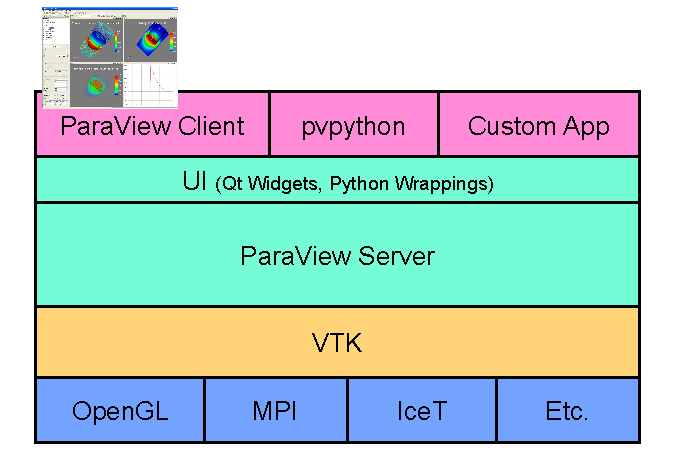
\includegraphics{images/ParaViewLibStack}
\end{inlinefig}

The application most people associate with ParaView is really just a small
client application built on top of a tall stack of libraries that provide
ParaView with its functionality.  Because the vast majority of ParaView
features are implemented in libraries, it is possible to completely replace
the ParaView GUI with your own custom application, as demonstrated in the
following figure.  Furthermore, ParaView comes with a \keyterm{pvpython}
application that allows you to automate the visualization and
post-processing with Python scripting.

Available to each ParaView application is a library of user interface
components to maximize code sharing between them.  A \keyterm{ParaView
  Server} library provides the abstraction layer necessary for running
parallel, interactive visualization.  It relieves the client application
from most of the issues concerning if and how ParaView is running in
parallel.  The \keyterm{Visualization Toolkit} (\keyterm{VTK}) provides the
basic visualization and rendering algorithms.  VTK incorporates several
other libraries to provide basic functionalities such as rendering,
parallel processing, file I/O, and parallel rendering.  Although this
tutorial demonstrates using ParaView through the ParaView client
application, be aware that the modular design of ParaView allows for a
great deal of flexibility and customization.

\section{Development and Funding}

The ParaView project started in 2000 as a collaborative effort between
Kitware Inc. and Los Alamos National Laboratory. The initial funding was
provided by a three year contract with the US Department of Energy ASCI
Views program.  The first public release, ParaView 0.6, was announced in
October 2002.  Development of ParaView continued through collaboration of
Kitware Inc. with Sandia National Laboratories, Los Alamos National
Laboratories, the Army Research Laboratory, and various other academic and
government institutions.

In September 2005, Kitware, Sandia National Labs and CSimSoft started the
development of ParaView 3.0. This was a major effort focused on rewriting
the user interface to be more user friendly and on developing a
quantitative analysis framework. ParaView 3.0 was released in May 2007.

Development of ParaView continues today.  Sandia National Laboratories
continues to fund ParaView development through the ASC project.  ParaView
is integrated as the major development platform for SciDAC Institute for
Ultra-Scale Visualization
(\href{http://www.ultravis.org}{www.ultravis.org}).  The US Department of
Energy also funds ParaView through Los Alamos National Laboratories, an
Army SBIR, and an ERDC contract.  The US National Science Foundation also
funds ParaView with an SBIR.  Other institutions also have ParaView support
contracts: Electricity de France, Mirarco, and oil industry customers.
Also, because ParaView is an open source project, other institutions such
as the Swiss National Supercomputing Centre contribute back their own
development.

\section{Basics of Visualization}

\begin{inlinefig}
  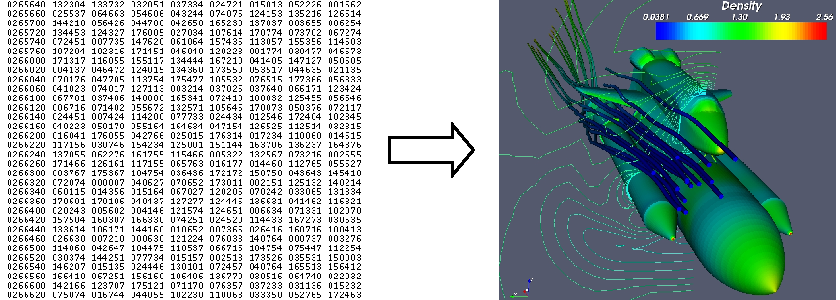
\includegraphics[width=\linewidth]{images/BasicsOfVisualization}
\end{inlinefig}

Put simply, the process of visualization is taking raw data and converting
it to a form that is viewable and understandable to humans.  This allows us
to get a better cognitive understanding of our data.  Scientific
visualization is specifically concerned with the type of data that has a
well defined representation in 2D or 3D space.  Data that comes from
simulation meshes and scanner data is well suited for this type of
analysis.

There are three basic steps to visualizing your data: reading, filtering,
and rendering.  First, your data must be read into ParaView.  Next, you may
apply any number of \keyterm{filters} that process the data to generate,
extract, or derive features from the data.  Finally, a viewable image is
rendered from the data.

ParaView was designed primarily to handle data with spatial
representation. Thus the primary \keyterm{data types} used in ParaView are
meshes.

\noindent
\begin{tabularx}{\linewidth}{p{2in}X}
  \parbox{2in}{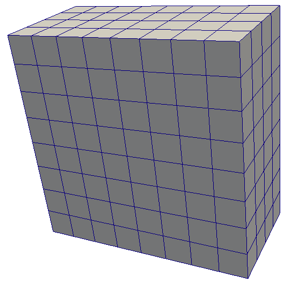
\includegraphics[width=2in]{images/ImageData}} &
  \begin{minipage}{\linewidth}
    \keyterm{Uniform Rectilinear (Image Data)}

    A uniform rectilinear grid is a one- two- or three- dimensional array of
    data.  The points are orthonormal to each other and are spaced regularly
    along each direction.
  \end{minipage}
\end{tabularx}

\noindent
\begin{tabularx}{\linewidth}{p{2in}X}
  \parbox{2in}{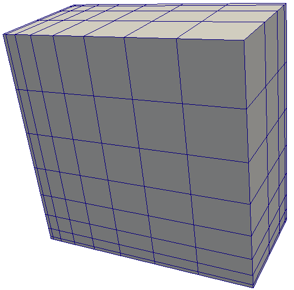
\includegraphics[width=2in]{images/RectilinearGrid}} &
  \begin{minipage}{\linewidth}
    \keyterm{Non-uniform Rectilinear (Rectilinear Grid)}

    Similar to the uniform rectilinear grid except that the spacing between
    points may vary along each axis.
  \end{minipage}
\end{tabularx}

\noindent
\begin{tabularx}{\linewidth}{p{2in}X}
  \parbox{2in}{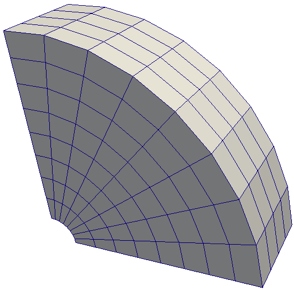
\includegraphics[width=2in]{images/StructuredGrid}} &
  \begin{minipage}{\linewidth}
    \keyterm{Curvilinear (Structured Grid)}

    Curvilinear grids have the same topology as rectilinear grids.
    However, each point in a curvilinear grid can be placed at an arbitrary
    coordinate (provided that it does not result in cells that overlap or
    self intersect).  Curvilinear grids provide the more compact memory
    footprint and implicit topology of the rectilinear grids, but also
    allow for much more variation in the shape of the mesh.
  \end{minipage}
\end{tabularx}

\noindent
\begin{tabularx}{\linewidth}{p{2in}X}
  \parbox{2in}{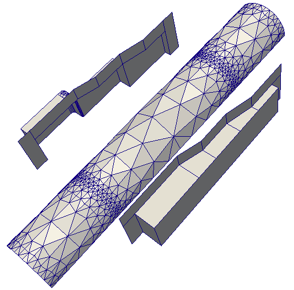
\includegraphics[width=2in]{images/PolyData}} &
  \begin{minipage}{\linewidth}
    \keyterm{Polygonal (Poly Data)}

    Polygonal data sets are composed of points, lines, and 2D polygons.
    Connections between cells can be arbitrary or non-existent.
    
    Polygonal data represents the basic rendering primitives.  Any data
    must be converted to polygonal data before being rendered (unless
    volume rendering is employed), although ParaView will automatically
    make this conversion.
  \end{minipage}
\end{tabularx}

\noindent
\begin{tabularx}{\linewidth}{p{2in}X}
  \parbox{2in}{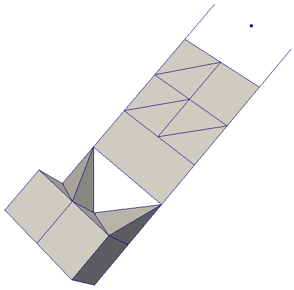
\includegraphics[width=2in]{images/UnstructuredGrid}} &
  \begin{minipage}{\linewidth}
    \keyterm{Unstructured Grid}

    Unstructured data sets are composed of points, lines, 2D polygons, 3D
    tetrahedra, and nonlinear cells.  They are similar to polygonal data
    except that they can also represent 3D tetrahedra and nonlinear cells,
    which cannot be directly rendered.
  \end{minipage}
\end{tabularx}

In addition to these basic data types, ParaView also supports
\keyterm{multi-block} data.  A basic multi-block data set is created
whenever data sets are grouped together or whenever a file containing
multiple blocks is read.  ParaView also has some special data types for
representing \keyterm{Hierarchical Adaptive Mesh Refinement}
(\keyterm{AMR}), \keyterm{Hierarchical Uniform AMR}, \keyterm{Octree},
\keyterm{Tablular} and \keyterm{Graph} type data sets


\section{More Information}

There are many places to find more information about ParaView.  For
starters, ParaView has online help that can be accessed by simply clicking
the \icon{pqHelp32} button in the application.  In addition to the on-line
help, \emph{The ParaView Guide} written by Amy Henderson Squillacote and
available from Kitware is a helpful guide for all things ParaView.

The ParaView web page, \href{http://www.paraview.org}{www.paraview.org}, is
also an excellent place to find more information about ParaView.  From
there you can find helpful links to mailing lists, Wiki pages, and
frequently asked questions as well as information about professional
support services.



% Chapter Introduction


\chapter{Basic Usage}
\label{chap:BasicUsage}

Let us get started using ParaView.  In order to follow along, you will need
your own installation of ParaView.  Specifically, this document is based
off of ParaView version \pvversion.  If you do not already have ParaView
\pvversion, you can download a copy from
\href{http://www.paraview.org}{www.paraview.org} (click on the download
link).  ParaView launches like most other applications.  On Windows, the
launcher is located in the start menu.  On Macintosh, open the application
bundle that you installed.  On Linux, execute \texttt{paraview} from a
command prompt (you may need to set your path).

The examples in this tutorial also rely on some data that is available at
\href{http://www.paraview.org/Wiki/ParaView_Tutorial}{http://www.paraview.org/Wiki/ParaView\_Tutorial}.
You may install this data into any directory that you like, but make sure
that you can find that directory easily.  Any time the tutorial asks you to
load a file it will be from the directory you installed this data in.


\section{User Interface}

\begin{inlinefig}
  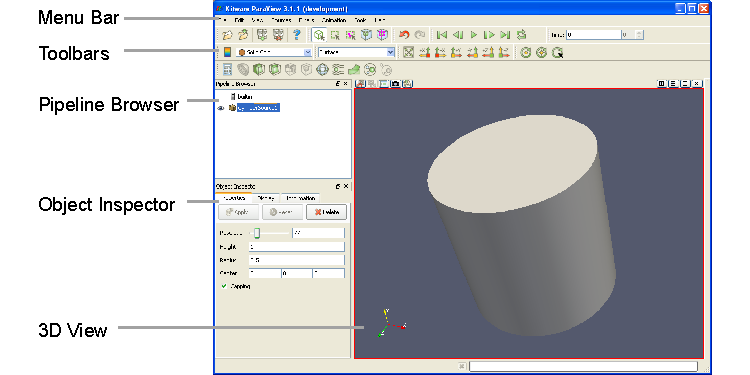
\includegraphics{images/UserInterface}
\end{inlinefig}

The ParaView GUI conforms to the platform on which it is running, but on
all platforms it behaves basically the same.  The layout shown here is the
default layout given when ParaView is first started.  The GUI comprises the
following components.

\begin{description}
\item[Menu Bar] \index{menu bar} As with just about any other program, the
  menu bar allows you to access the majority of features.
\item[Toolbars] \index{toolbars} The toolbars provide quick access to the
  most commonly used features within ParaView.
\item[Pipeline Browser] \index{pipeline browser} ParaView manages the
  reading and filtering of data with a pipeline.  The pipeline browser
  allows you to view the pipeline structure and select pipeline objects.
  Redesigned for ParaView 3, the pipeline browser provides a convenient
  list of pipeline objects with an indentation style that shows the
  pipeline structure.
\item[Object Inspector] \index{object inspector} The object inspector
  allows you to view and change the parameters of the current pipeline
  object.  There are three tabs in the object inspector.  The
  \keyterm{Properties} tab presents the configurable options for the object
  behavior.  The \keyterm{Display} tab presents options for how the object
  is represented in the view.  The \keyterm{Information} tab shows basic
  statistics on the data produced by the pipeline object.
\item[3D View] \index{3D View} The remainder of the GUI is used to present
  data so that you may view, interact with, and explore your data.  This
  area is initially populated with a 3D view that will provide a geometric
  representation of the data.
\end{description}

Note that the GUI layout is highly configurable, so that it is easy to
change the look of the window.  The toolbars can be moved around and even
hidden from view.  To toggle the use of a toolbar, use the \gui{View} \ra
\gui{Toolbars} submenu.  The pipeline browser and object inspector are both
\keyterm{dockable} windows.  This means that these components can be moved
around in the GUI, torn off as their own floating windows, or hidden
altogether.  These two windows are important to the operation of ParaView,
so if you hide them and then need them again, you can get them back with
the \gui{View} menu.


\section{Sources}

There are two ways to get data into ParaView: read data from a file or
generate data with a \keyterm{source} object.  All sources are located in
the \gui{Sources} menu.  Sources can be used to add annotation to a view,
but they are also very handy when exploring ParaView’s features.

\begin{exercise}{Creating a Source}
  \label{ex:CreatingASource}%
  Let us start with a simple one.  Go to the \gui{Sources} menu and select
  \gui{Cylinder}.  Once you select the \gui{Cylinder} item you will notice
  that an item named \gui{Cylinder1} is added to and selected in the
  pipeline browser.  You will also notice that the object inspector is
  filled with the properties for the cylinder source.  Click the
  \gui{Apply} button \apply to accept the default parameters.

  Once you click \gui{Apply}, the cylinder object will be displayed in the
  3D view window on the right.  You can manipulate this 3D view by dragging
  the mouse over the 3D view.  Experiment with dragging different mouse
  buttons---left, middle, and right---to perform different rotate, pan, and
  zoom operations.  Also try using the buttons in conjunction with the
  shift and ctrl modifier keys.

  You will quickly notice that ParaView creates not a real cylinder but
  rather an approximation of a cylinder using polygonal \keyterm{facets}.
  The default parameters for the cylinder source provide a very coarse
  approximation of only six facets. (In fact, this object looks more like a
  prism than a cylinder.) If we want a better representation of a cylinder,
  we can create one by increasing the \gui{Resolution} parameter.

  \begin{inlinefig}
    
\includegraphics[width=2.5in]{images/ResolutionParameter}
  \end{inlinefig}

  Using either the slider or text edit, increase the resolution to 50 or
  more.  Notice that the \gui{Apply} button \apply has turned green (or
  blue on Mac) again.  This is because changes you make to the object
  inspector are not immediately enacted.  The highlighted button is a
  reminder that the parameters of one or more pipeline objects are ``out of
  sync'' with the data that you are viewing.  Hitting the \gui{Apply} button
  will accept these changes whereas hitting the \gui{Reset} button \reset
  will revert the options back to the last time they were applied.  Hit the
  \gui{Apply} button now.  The resolution is changed so that it is
  virtually indistinguishable from a true cylinder.
\end{exercise}

Now is a good time to note the undo~\icon{pqUndo32} and
redo~\icon{pqRedo32} buttons in the toolbar.  Visualizing your data is
often an exploratory process, and it is often helpful to revert back to a
previous state.  You can even undo back to the point before your data was
created and redo again.

\begin{exercise}{Undo and Redo}
  \label{ex:UndoAndRedo}%
  Experiment with the undo~\icon{pqUndo32} and redo~\icon{pqRedo32}
  buttons.  If you have not done so, create and modify a pipeline object
  like what is done in Exercise~\ref{ex:CreatingASource}.  Watch how
  parameter changes can be reverted and restored.  Also notice how whole
  pipeline objects can be destroyed and recreated.

  There are also special undo camera~\icon{pqUndoCamera24} and redo
  camera~\icon{pqRedoCamera24} buttons.  These allow you to go back and
  forth between camera angles that you have made so that you no longer have
  to worry about errant mouse movements ruining that perfect view.  Move
  the camera around and then use these buttons to revert and restore the
  camera angle.
\end{exercise}

There are also many options for selecting how objects are rendered.  You
will notice over the 3D view a \icon{pqOptions16} button for changing the
rendering options.  Clicking this brings up a dialog box that allows you to
change things like the background color, the lighting, and annotation.

\begin{inlinefig}
  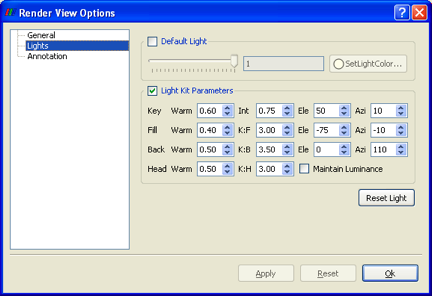
\includegraphics[width=3in]{images/RenderViewOptions}
\end{inlinefig}

Another location for rendering options is the \gui{Display} tab in the
object inspector.  This tab provides the rendering options that apply
specifically for the selected object.  It includes the visibility,
coloring, and representation.  Be aware that some of the view options and
object display options are repeated elsewhere in the ParaView GUI for
convenience.

\begin{inlinefig}
  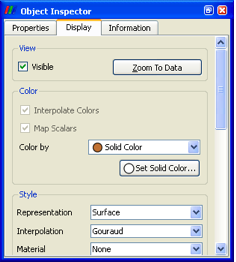
\includegraphics[width=1.6in]{images/DisplayTab}
\end{inlinefig}

\begin{exercise}{Modifying Rendering Parameters}
  \label{ex:ModifyingRenderingParameters}%
  Click the \icon{pqOptions16} button above the 3D view to bring up the
  \gui{Render View Options} dialog box.  Explore the different panels of
  options.  Try modifying how the view looks in the following ways.
  (Remember that you will have to hit \gui{Apply} or \gui{OK} before the
  changes take effect.)

  \begin{itemize}
  \item Change the background color.  (Notice that you can reset it to the
    default.)
  \item Turn the Orientation Axis (the axis in the lower left corner of the
    view) off and on.
  \item Move the Orientation Axis in the view.  (Hint: Make the axis
    interactive and then click and drag in the 3D view.)
  \end{itemize}

  Now change the drawing parameters of the cylinder.  (If you do not have a
  cylinder or another pipeline object, create one as described in
  Exercise~\ref{ex:CreatingASource}.)  Make sure the cylinder is selected
  in the pipeline browser.  In the object inspector, select the
  \gui{Display} tab.

  \begin{itemize}
  \item Set the (solid) color of the cylinder.  (Note: You can also set the
    color with the \icon{pqEditColor24} toolbar button.)
  \item Make the cylinder shiny.  (Hint: Make the \gui{Specular Intensity}
    1.0.)
  \item Make the cylinder transparent.  (Hint: Lower the \gui{Opacity}.)
  \item Show 3D axes with tic marks giving spatial position (\gui{Show cube
    axes}).
  \end{itemize}

  We are done with the cylinder source now.  We can delete the pipeline
  object by selecting the \gui{Properties} tab and hitting delete \delete
  in the object inspector.
\end{exercise}


\section{Loading Data}

Now that we have had some practice using the ParaView GUI, let us load in
some real data.  As you would expect, the \gui{Open} command is the first
one off of the \gui{File} menu, and there is also toolbar
button~\icon{pqOpen32} for opening a file.  ParaView supports many file
types, and the list grows as more types get added.  The following is a list
of currently available readers.

\begin{multicols}{2}
  \begin{itemize}
  \item ParaView Data (.pvd)
  \item VTK (.vtp, .vtu, .vti, .vts, .vtr)
  \item VTK Multi Block (.vtm, .vtmb, .vtmg, .vthd, .vthb)
  \item Partitioned VTK (.pvtu, .pvti, .pvts, .pvtr)
  \item VTK Legacy (.vtk)
  \item Exodus
  \item XDMF (.xmf, .xdmf)
  \item LS-DYNA
  \item SpyPlot CTH
  \item EnSight (.case, .sos)
  \item netCDF (.ncdf, .nc)
  \item BYU (.g)
  \item Protein Data Bank (.pdb)
  \item XMol Molecule
  \item PLOT3D
  \item Digital Elevation Map (.dem)
  \item VRML (.wrl)
  \item PLY Polygonal File Format
  \item Stereo Lithography (.stl)
  \item Gaussian Cube File (.cube)
  \item POP Ocean Files
  \item AVS UCD (.inp)
  \item Meta Image (.mhd, .mha)
  \item Facet Polygonal Data
  \item Phasta Files (.pht)
  \item SESAME Tables
  \item MFIX (.RES)
  \item Fluent Case Files (.cas)
  \item OpenFOAM Files (.foam)
  \item Cosmology Files (.cosmo)
  \item PNG Image Files
  \item TIFF Image Files
  \item Raw Image Files
  \item Comma Separated Values (.csv)
  \end{itemize}
\end{multicols}

ParaView’s modular design allows for easy integration of new VTK readers
into ParaView.  Thus, check back often for new file formats.  If you are
looking for a file reader that does not seem to be included with ParaView,
check in with the ParaView mailing list
(\href{mailto:paraview@paraview.org}{paraview@paraview.org}).  There are
many file readers included with VTK but not exposed within ParaView that
could easily be added.  There are also many readers created that can plug
into the VTK framework but have not been committed back to VTK; someone may
have a reader readily available that you can use.

\begin{exercise}{Opening a File}
  \label{ex:OpeningAFile}%
  Let us open our first file now.  Click the \gui{Open} toolbar (or menu
  item)~\icon{pqOpen32} and open the file \gui{disk\_out\_ref.ex2}.  Note
  that opening a file is a two step process, so that you do not see any
  data yet.  Instead, you see that the object inspector is populated with
  several options about how we want to read the data.

  \begin{inlinefig}
    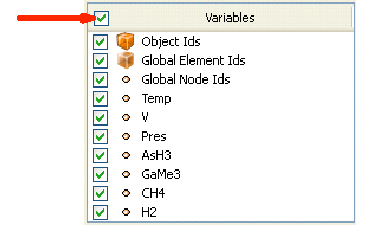
\includegraphics{images/Variables_disk_out_ref}
  \end{inlinefig}

  Click the checkbox in the header of the variable list to turn on the
  loading of all the variables.  This is a small data set, so we do not
  have to worry about loading too much into memory.  Once all of the
  variables are selected, click \apply to load all of the data.  When the
  data is loaded you will see that the geometry looks like a cylinder with
  a hollowed out portion in one end.  This data is the output of a
  simulation for the flow of air around a heated and spinning disk.  The
  mesh you are seeing is the air around the disk (with the cylinder shape
  being the boundary of the simulation.  The hollow area in the middle is
  where the heated disk would be were it meshed for the simulation.
\end{exercise}

Before we continue on to filtering the data, let us take a quick look at
some of the ways to represent the data.  The most common parameters for
representing data are located in a pair of toolbars.

\begin{inlinefig}
  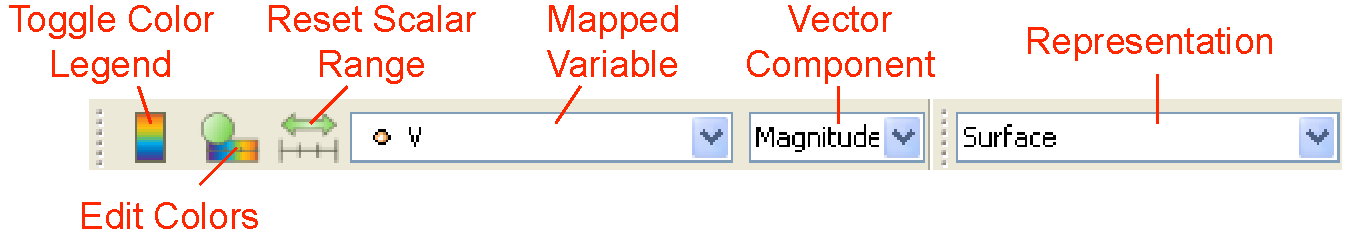
\includegraphics[width=\linewidth]{images/DataRepresentationToolbars}
\end{inlinefig}

\begin{exercise}{Representation and Field Coloring}
  \label{ex:RepresentationAndFieldColoring}%
  Play with the data representation a bit.  Make sure
  \gui{disk\_out\_ref.ex2} is selected in the pipeline browser.  (If you do
  not have the data loaded, repeat Exercise~\ref{ex:OpeningAFile}.)  Use
  the variable chooser to color the surface by the \gui{Pres} variable.
  Then turn the color legend on to see the actual pressure values.  To see
  the structure of the mesh, change the representation to \gui{Surface With
    Edges}.  You can view both the cell structure and the interior of the
  mesh with the \gui{Wireframe} representation.

  \begin{inlinefig}
    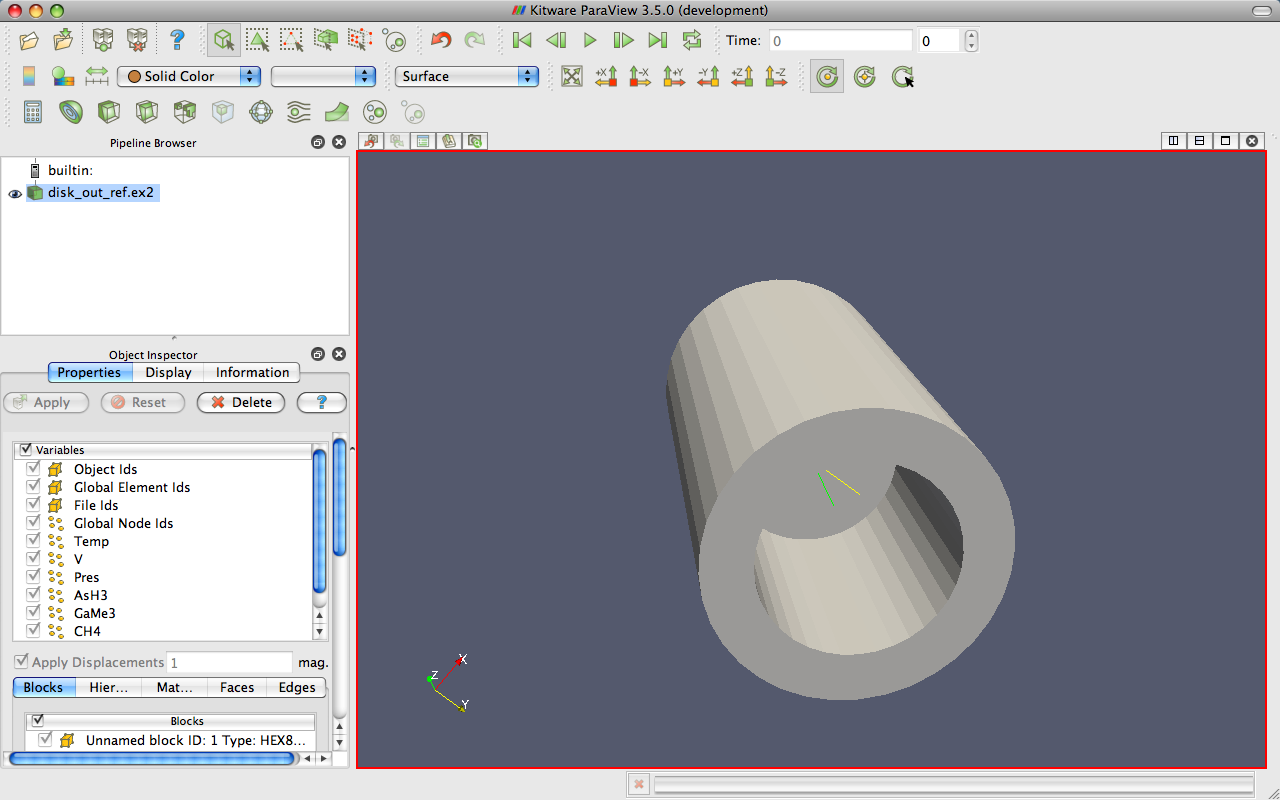
\includegraphics[width=2.25in]{images/DataRepresentation1}
    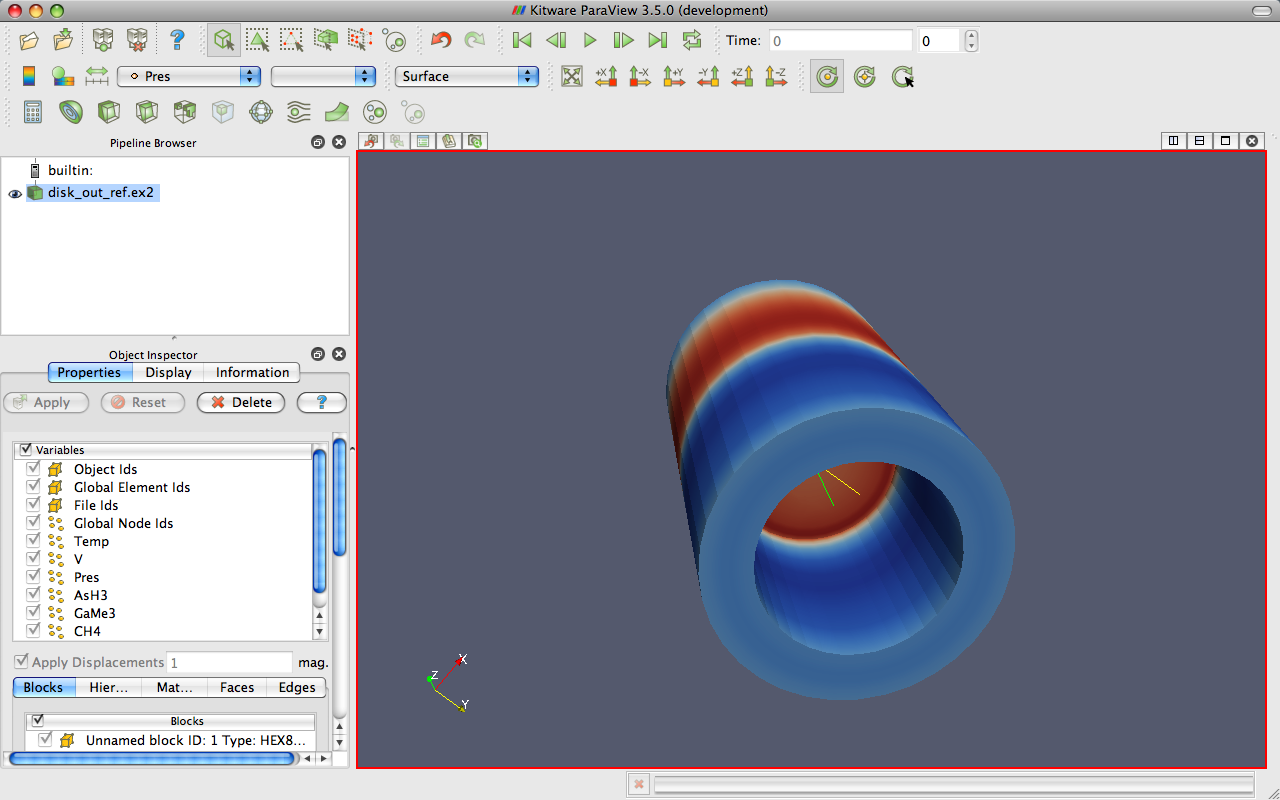
\includegraphics[width=2.25in]{images/DataRepresentation2} \\
    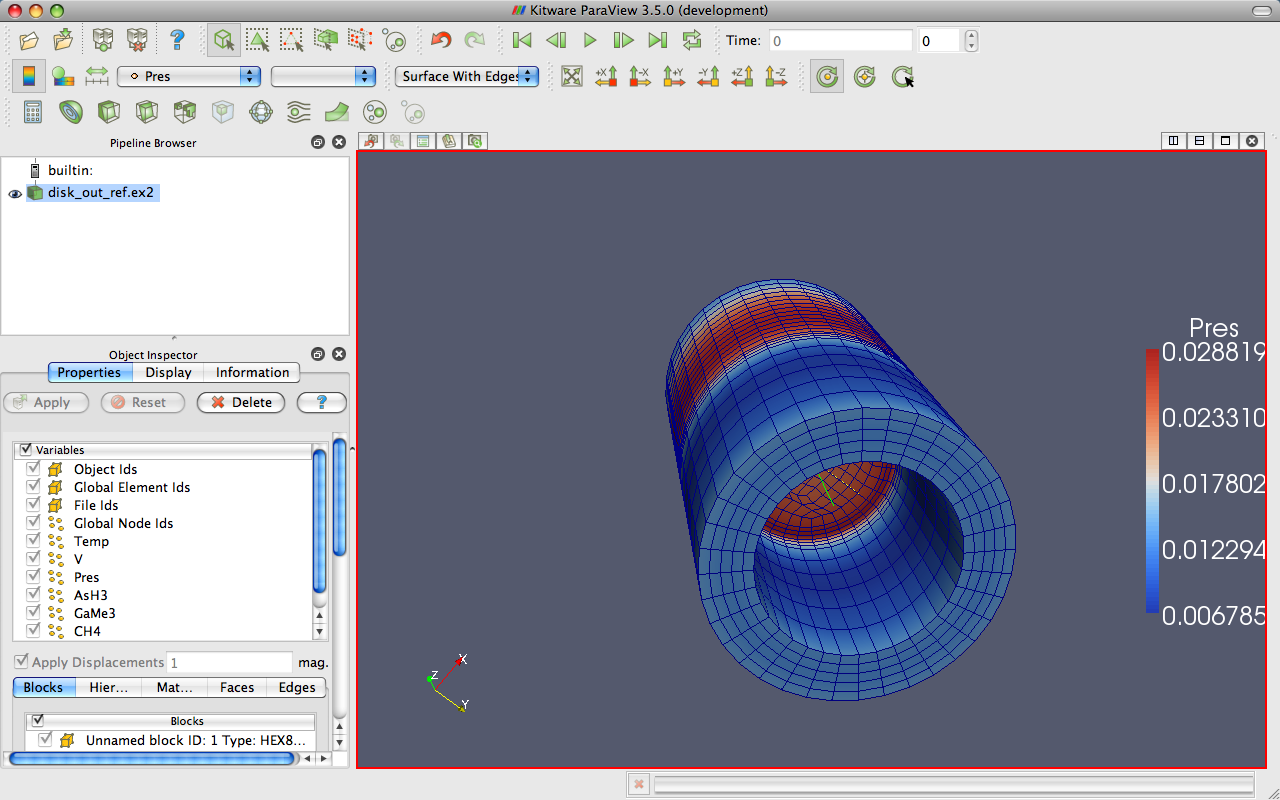
\includegraphics[width=2.25in]{images/DataRepresentation3}
    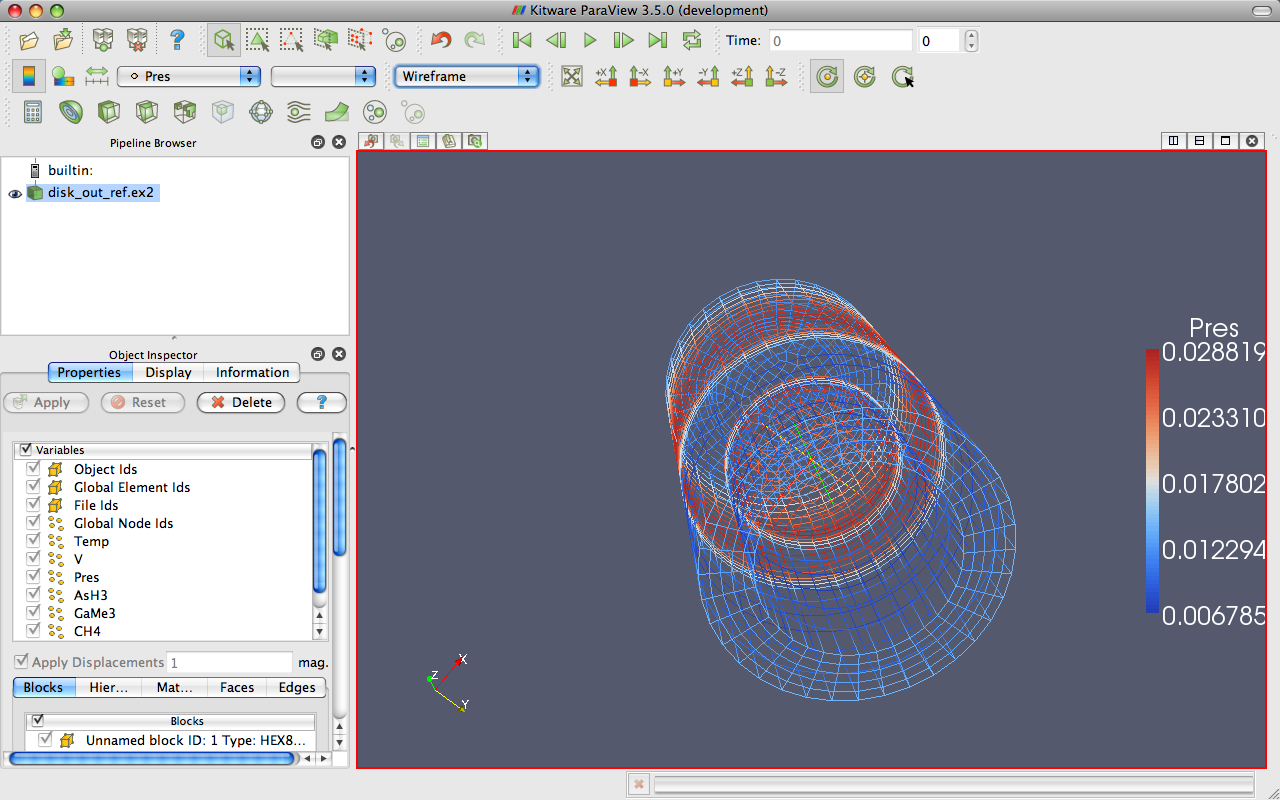
\includegraphics[width=2.25in]{images/DataRepresentation4}
  \end{inlinefig}
\end{exercise}


\section{Filters}

We have now successfully read in some data and gleaned some information
about it.  We can see the basic structure of the mesh and map some data
onto the surface of the mesh.  However, as we will soon see, there are many
interesting features about this data that we cannot determine by simply
looking at the surface of this data.  There are many variables associated
with the mesh of different types (scalars and vectors).  And remember that
the mesh is a solid model.  Most of the interesting information is on the
inside.

We can discover much more about our data by applying \keyterm{filters}.
Filters are functional units that process the data to generate, extract, or
derive features from the data.  Filters are attached to readers, sources,
or other filters to modify its data in some way.  These filter connections
form a \keyterm{visualization pipeline}.  There are a great many filters
available in ParaView.  Here are the most common, which are all available
by clicking on the respective icon in the filters toolbar.

\begin{description}
\item[\calculator Calculator] \index{calculator} Evaluates a user-defined
  expression on a per-point or per-cell basis.
\item[\contour Contour] \index{contour} Extracts the points, curves, or
  surfaces where a scalar field is equal to a user-defined value.  This
  surface is often also called an \keyterm{isosurface}.
\item[\clip Clip] \index{clip} Intersects the geometry with a half space.
  The effect is to remove all the geometry on one side of a user-defined
  plane.
\item[\slice Slice] \index{slice} \index{cut|see{slice}} Intersects the
  geometry with a plane.  The effect is similar to clipping except that all
  that remains is the geometry where the plane is located.
\item[\threshold Threshold] \index{threshold} Extracts cells that lie
  within a specified range of a scalar field.
\item[\extractSubset Extract Subset] \index{extract subset} Extracts a
  subset of a grid by defining either a volume of interest or a sampling
  rate.
\item[\glyph Glyph] Places a \keyterm{glyph}, a simple shape, on each point
  in a mesh.  The glyphs may be oriented by a vector and scaled by a vector
  or scalar.
\item[\streamTracer Stream Tracer] \index{stream tracer} Seeds a vector
  field with points and then traces those seed points through the (steady
  state) vector field.
\item[\warp Warp (vector)] \index{warp!vector} Displaces each point in a
  mesh by a given vector field.
\item[\group Group Datasets] \index{group datasets} Combines the output of
  several pipeline objects into a single multi block data set.
\item[\extractGroup Extract Group] \index{extract group} Extract one or
  more items from a multi block data set.
\end{description}

\parpic[r]{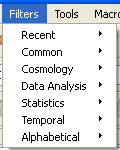
\includegraphics[width=2in]{images/FiltersMenu}}

These eleven filters are a small sampling of what is available in ParaView.
In the \gui{Filters} menu are a great many more filters that you can use to
process your data.  ParaView currently exposes over eighty filters, so to
make them easier to find the \gui{Filters} menu is organized into submenus.
These submenus are organized as follows.

\begin{description}
\item[Recent] The list of most recently used filters sorted with the most
  recently used filters on top.
\item[Common] The most common filters.  This is the same list of filters
  available in the filters toolbar and listed previously.
\item[Data Analysis] The filters designed to retrieve quantitative values
  from the data.  These filters compute data on the mesh, extract elements
  from the mesh, or plot data.
\item[Temporal] Filters that analyze or modify data that changes over time.
  All filters can work on data that changes over time because they are
  executed on each time snapshot.  However, filters in this category will
  introspect the available time extents and examine how data changes over
  time.
\item[Alphabetical] An alphabetical listing of all the filters available.
  If you are not sure where to find a particular filter, this list is
  guaranteed to have it.  There are also many filters that are not listed
  anywhere but in this list.
\end{description}

\parpic[r]{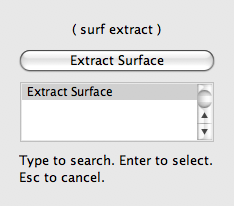
\includegraphics[width=2.5in]{images/QuickLaunch}}

Searching through these lists of filters, particularly the full
alphabetical list, can be cumbersome.  To speed up the selection of
filters, you should use the \keyterm{quick launch} dialog.  When the ctrl
and space keys together on Windows or Linux or the alt and space keys
together on Macintosh, ParaView brings up a small, lightweight dialog box
like the one shown here.  Type in words or word fragments that are
contained in the filter name, and the box will list only those sources and
filters that match the terms.  Hit enter to add the object to the pipeline
browser.

You have probably noticed that some of the filters are grayed out.  Many
filters only work on a specific types of data and therefore cannot always
be used.  ParaView disables these filters from the menu and toolbars to
indicate (and enforce) that you cannot use these filters.

Throughout this tutorial we will explore many filters.  However, we cannot
explore all the filters in this forum.  Consult \emph{The ParaView Guide}
for more information on each filter.

\begin{exercise}{Apply a Filter}
  \label{ex:ApplyAFilter}%
  Let us apply our first filter.  If you do not have the disk\_out\_ref.ex2
  data loaded, do so know (Exercise~\ref{ex:OpeningAFile}).  Make sure that
  \gui{disk\_out\_ref.ex2} is selected in the pipeline browser and then
  select the contour filter~\contour from the filter toolbar or
  \gui{Filters} menu.  Notice that a new item is added to the pipeline
  filter underneath the reader and the object inspector updates to the
  parameters of the new filter.  As with reading a file, applying a filter
  is a two step process.  After creating the filter you get a chance to
  modify the parameters (which you will almost always do) before applying
  the filter.

  \begin{inlinefig}
    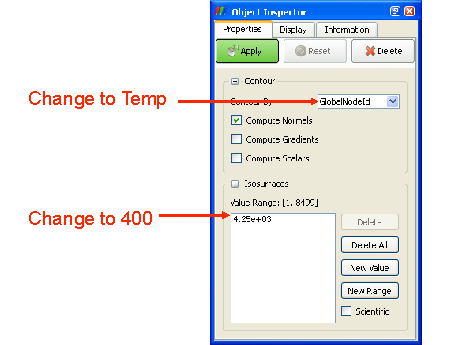
\includegraphics{images/ContourOptions}
  \end{inlinefig}

  We will use the contour filter to create an isosurface where the
  temperature is equal to 400 K.  First, change the \gui{Contour By}
  parameter to the \gui{Temp} variable.  Then, change the isosurface value
  to \gui{400}.  Finally, hit \apply.  You will see the isosurface appear
  inside of the volume.  If \gui{disk\_out\_ref.ex2} was still colored by
  pressure from Exercise~\ref{ex:RepresentationAndFieldColoring}, then the
  surface is colored by pressure to match.

  \begin{inlinefig}
    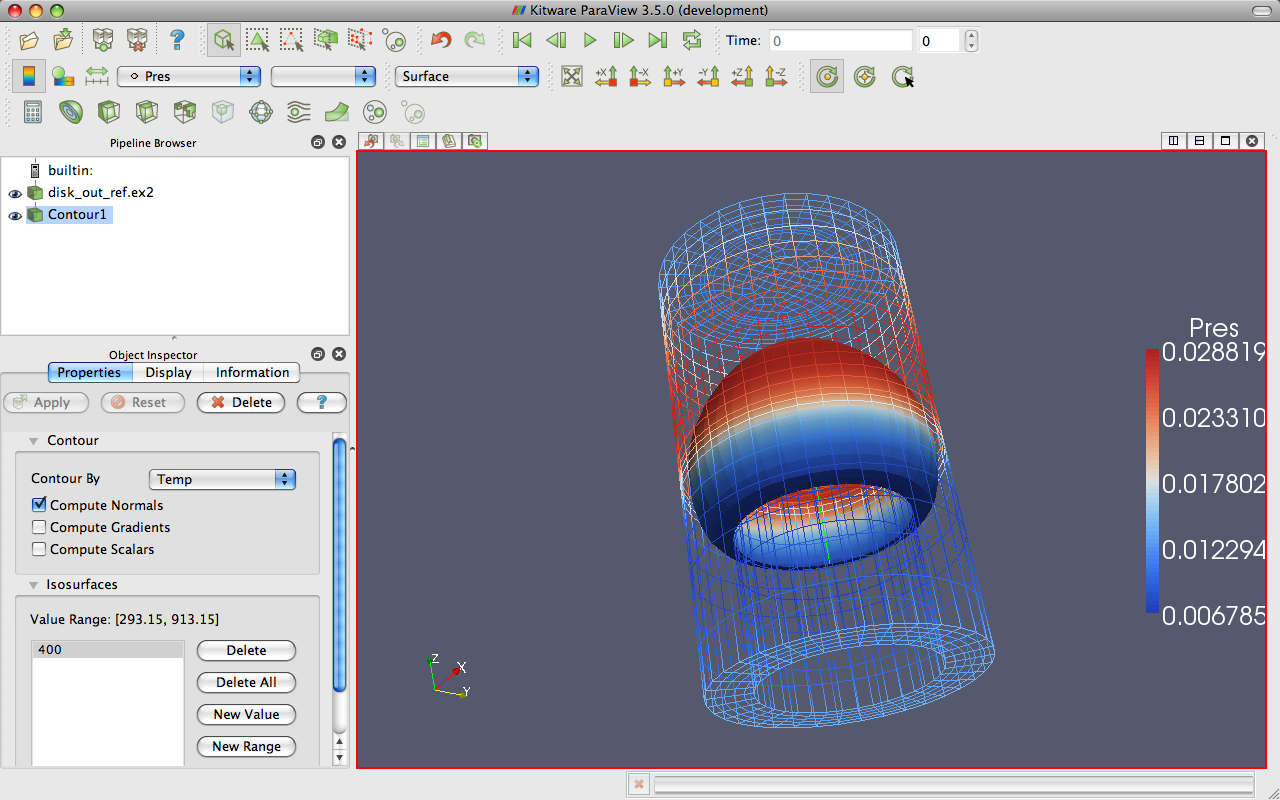
\includegraphics[width=3in]{images/ContourResults}
  \end{inlinefig}
\end{exercise}

In the preceding exercise, we applied a filter that processed the data and
gave us the results we needed.  For most common operations, a single filter
operation is sufficient to get the information we need.  However, filters
are of the same class as readers.  That is, the general operations we apply
to readers can also be applied to filters.  Thus, you can apply one filter
to the data that is generated by another filter.  These readers and filters
connected together form what we call a \keyterm{visualization pipeline}.
The ability to form visualization pipelines provides a powerful mechanism
for customizing the visualization to your needs.

Let us play with some more filters.  Rather than show the mesh surface in
wireframe, which often interferes with the view of what is inside it, we
will replace it with a cutaway of the surface.  We need to filters to
perform this task.  The first filter will extract the surface, and the
second filter will cut some away.

\begin{exercise}{Creating a Visualization Pipeline}
  \label{ex:CreatingAVisualizationPipeline}%
  The images and some of the discussion in this exercise assume you are
  starting with the state right after finishing
  Exercise~\ref{ex:ApplyAFilter}.  If you have had to restart ParaView
  since or your state does not match up well enough, it is sufficient to
  simply have disk\_out\_ref.ex2 loaded.

  Start by adding a filter that will extract the surfaces.  We do that with
  the following steps.

  \begin{enumerate}
  \item Select \gui{disk\_out\_ref.ex2} in the pipeline browser.
  \item From the menu bar, select \gui{Filters} \ra \gui{Alphabetical} \ra
    \gui{Extract Surface}. \index{extract surface} Or bring up the quick
    launch (ctrl+space Win/Linux, alt+space Mac), type extract surface, and
    select that filter.
  \item Hit the \apply button.
    \savecounter
  \end{enumerate}

  \begin{inlinefig}
    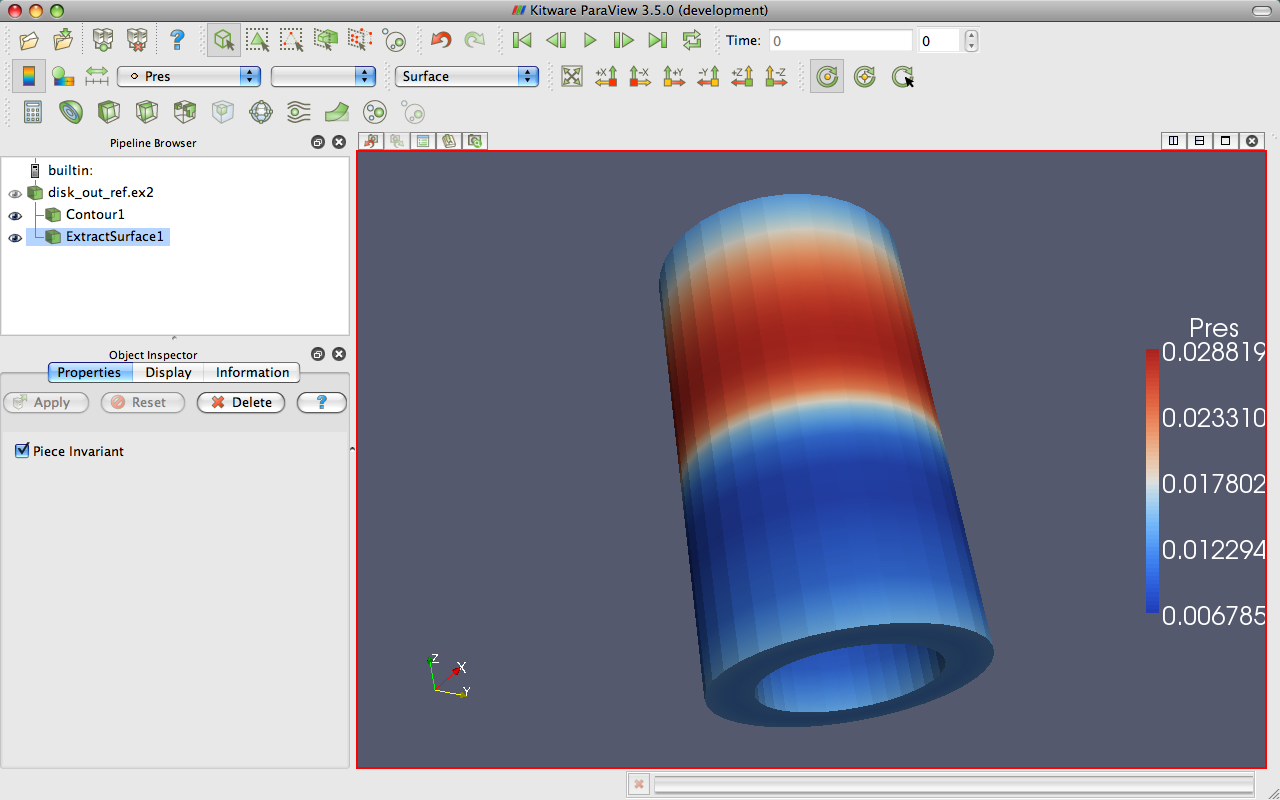
\includegraphics[width=3in]{images/CutSurface1}
  \end{inlinefig}

  When you apply the \gui{Extract Surface} filter, you will once again see
  the surface of the mesh.  Although it looks like the original mesh, it is
  different in that this data is hollow whereas the original data was solid
  throughout.

  If you were showing the results of the contour filter, you cannot see the
  contour anymore, but do not worry.  It is still in there hidden by the
  surface.  If you are showing the contour but you did not see any effect
  after applying the filter, you may have forgotten step one and applied
  the filter to the wrong object.  If the \gui{ExtractSurface1} object is
  not connected directly to the \gui{disk\_out\_ref.ex2}, then this is what
  went wrong.  If so, you can delete the filter and try again.

  Now we will cut away the external surface to expose the internal
  structure and isosurface underneath (if you have one).

  \begin{enumerate}
    \restorecounter
  \item Verify that \gui{ExtractSurface1} is selected in the pipeline
    browser.
  \item Create a clip filter \clip from the toolbar or \gui{Filters} menu.
  \item Uncheck the \gui{Show Plane} checkbox
    \includeinlinegraphics{images/ShowPlaneCheckbox} in the object inspector.
  \item Click the \apply button.
  \end{enumerate}

  \begin{inlinefig}
    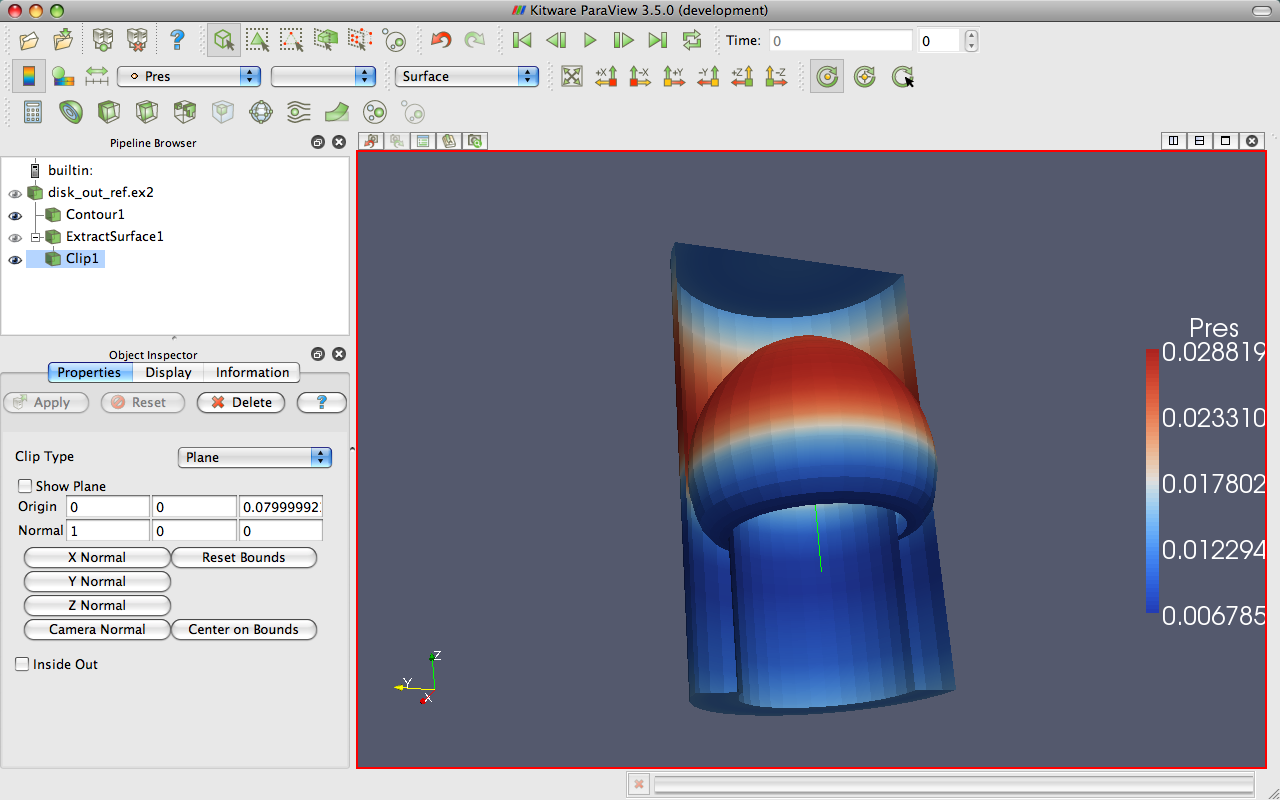
\includegraphics[width=3in]{images/CutSurface2}
  \end{inlinefig}

  If you have a contour, you should now see the isosurface contour within a
  cutaway of the mesh surface.  You will probably have to rotate the mesh
  to see the contour clearly.
\end{exercise}

\begin{inlinefig}
  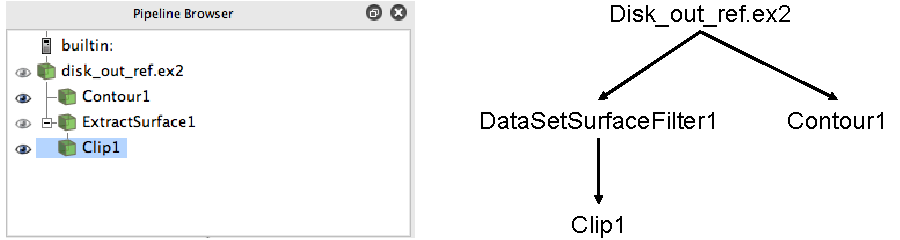
\includegraphics[width=\linewidth]{images/PipelineBrowserStructure}
\end{inlinefig}

Now that we have added several filters to our pipeline, let us take a look
at the layout of these filters in the pipeline browser.  The pipeline
browser provides a convenient list of pipeline objects that we have created
make it easy to select pipeline objects and change their
\keyterm{visibility} by clicking on the eyeball icons~\eyeball next to
them.  But also notice the indentation of the entries in the list and the
connecting lines toward the right.  These features reveal the
\keyterm{connectivity} of the pipeline.  It shows the same information as
the traditional graph layout on the right, but in a much more compact
space.  The trouble with the traditional layout of pipeline objects is that
it takes a lot of space, and even moderately sized pipelines require a
significant portion of the GUI to see fully.  The pipeline browser,
however, is complete and compact.


\section{Multiview}
\label{sec:Multiview}

Occasionally in the pursuit of science we can narrow our focus down to one
variable.  However, most interesting physical phenomena rely on not one but
many variables interacting in certain ways.  It can be very challenging to
present many variables in the same view.  To help you explore complicated
visualization data, ParaView contains the ability to present multiple views
of data and correlate them together.

So far in our visualization we are looking at two variables: We are
coloring with pressure and have extracted an isosurface with temperature.
Although we are starting to get the feel for the layout of these variables,
it is still difficult to make correlations between them.  To make this
correlation easier, we can use multiple views.  Each view can show an
independent aspect of the data and together they may show a more complete
understanding.

On top of each view is a small toolbar, and the buttons controlling the
creating and deletion of views are located on the right side of this tool
bar.  There are four buttons in all.  You can create a new view by
splitting an existing view horizontally or vertically with the \splitViewH
and \splitViewV buttons, respectively.  The \deleteView button deletes a
view, whose space is consumed by an adjacent view.  The \maximizeView
temporarily fills view space with the selected view until \restoreView is
pressed.

\begin{exercise}{Using Multiple Views}
  \label{ex:UsingMultipleViews}%
  We are going to start a fresh visualization, so if you have been
  following along with the exercises so far, now is a good time to reset
  ParaView.  The easiest way to do this is to press the~\disconnect button.
  We will discuss what this does later in more detail in
  Chapter~\ref{chap:VisualizingLargeModels}, but for now just know that it
  is roughly the equivalent of restarting ParaView.

  First, we will look at one variable.  We need to see the variable through
  the middle of the mesh, so we are going to clip the mesh in half.

  \begin{enumerate}
  \item Open the file disk\_out\_ref.ex2, load all variables, \apply (see
    Exercise~\ref{ex:OpeningAFile}).
  \item Add the Clip filter~\clip to \gui{disk\_out\_ref.ex2}.
  \item Uncheck the Show Plane checkbox
    \includeinlinegraphics{images/ShowPlaneCheckbox} in the object inspector.
  \item Click the \apply button.
  \item Color the surface by pressure by changing the variable chooser (in
    the toolbar) from \gui{Solid Color} to \gui{Pres}.
    \savecounter
  \end{enumerate}

  Now we can see the pressure in a plane through the middle of the mesh.
  We want to compare that to the temperature on the same plane.  To do
  that, we create a new view to build another visualization.

  \begin{enumerate}
    \restorecounter
  \item Press the \splitViewH button.
  \end{enumerate}

  \begin{inlinefig}
    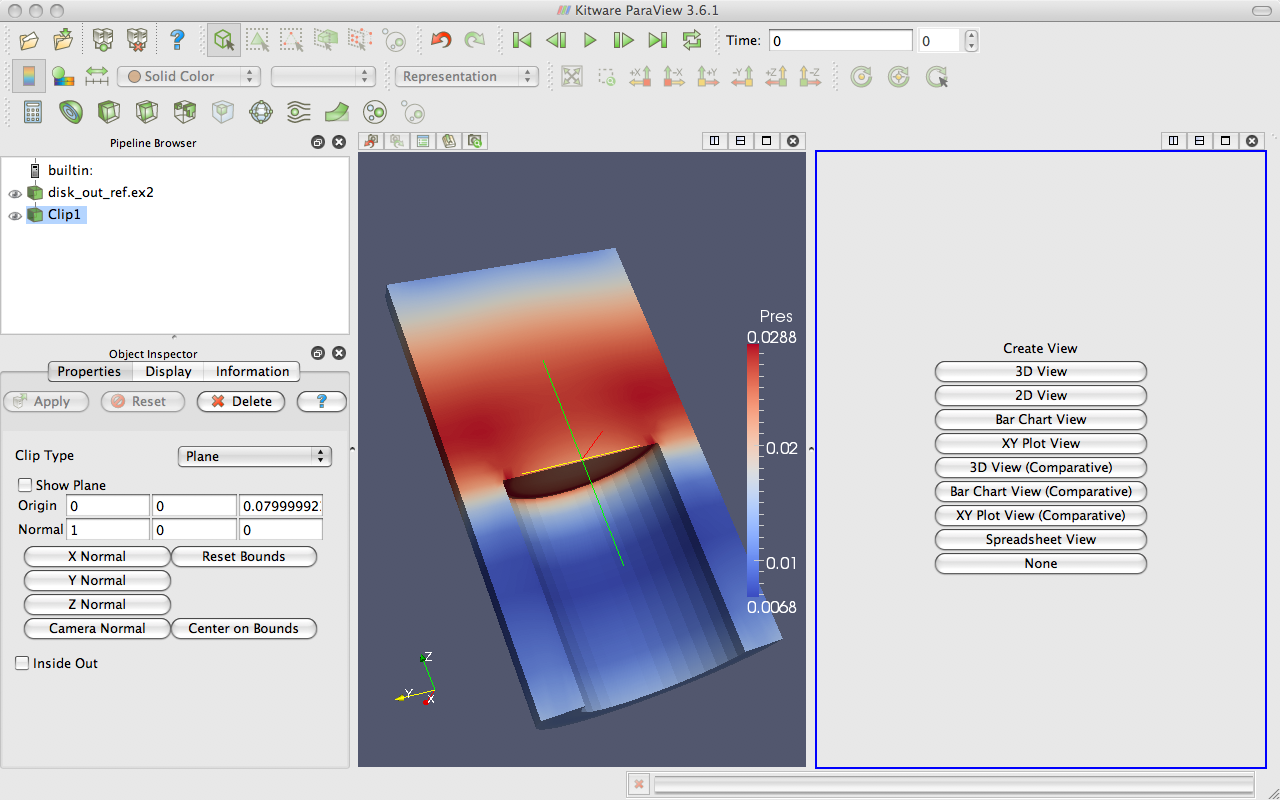
\includegraphics[width=3in]{images/SplitView1}
  \end{inlinefig}

  The current view is split in half and the right side is blank, ready to
  be filled with a new visualization.  Notice that the view in the right
  has a blue border around it.  This means that it is the \keyterm{active
    view}.  Widgets that give information about and controls for a single
  view, including the pipeline browser and object inspector, follow the
  active view.  In this new view we will visualize the temperature of the
  mesh.

  \begin{enumerate}
  \item Make sure the blue border is still around the new, blank view (to
    the right).  You can make any view the active view by simply clicking
    on it.
  \item Turn on the visibility of the clipped data by clicking the
    eyeball~\eyeballg next to \gui{Clip1} in the pipeline browser.
  \item Color the surface by temperature by selecting \gui{Clip1} in the
    pipeline browser and changing the variable chooser (in the toolbar)
    from \gui{Solid Color} to \gui{Temp} (you may want to turn on the color
    bar at this point as well).
    \savecounter
  \end{enumerate}

  \begin{inlinefig}
    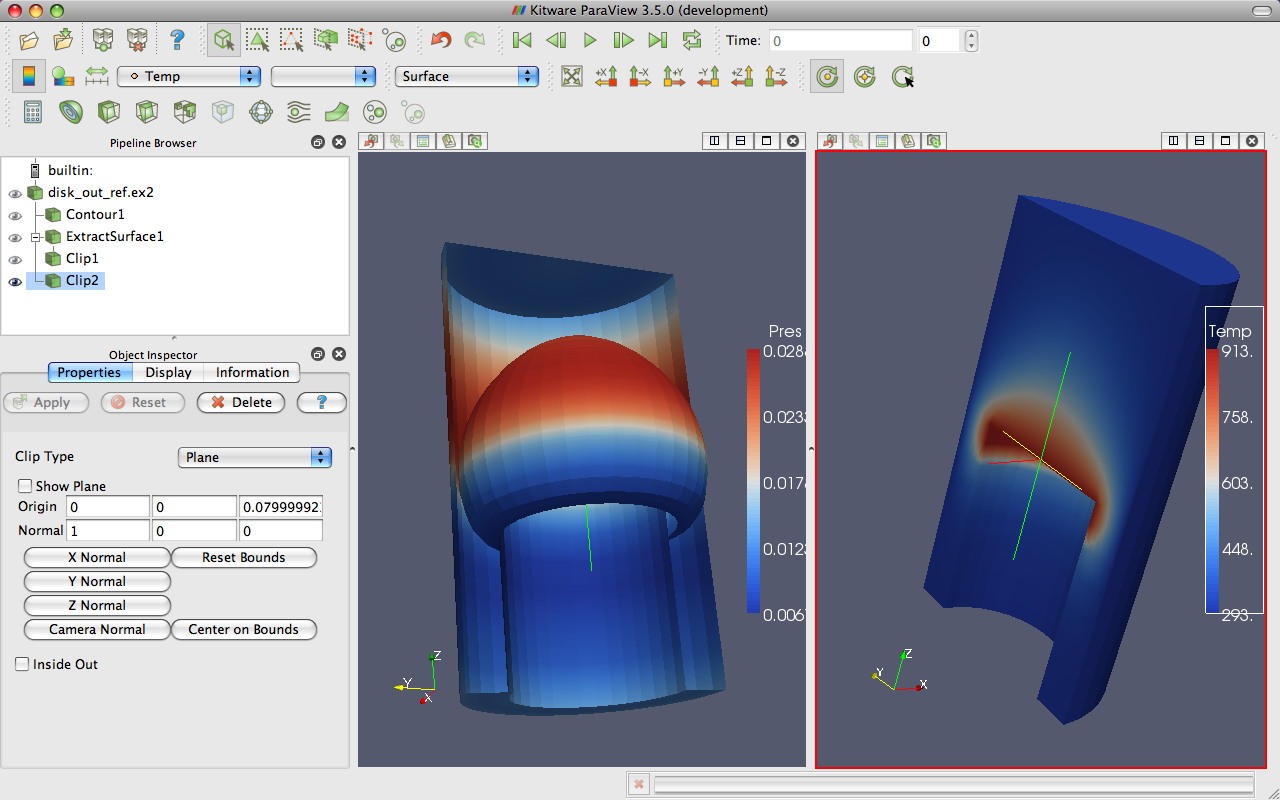
\includegraphics[width=3in]{images/SplitView2}
  \end{inlinefig}

  We now have two views: one showing information about pressure and the
  other information about temperature.  We would like to compare these, but
  it is difficult to do because the orientations are different.  How are we
  to know how a location in one correlates to a location in the other?  We
  can solve this problem by adding a \keyterm{camera link} so that the two
  views will always be drawn from the same viewpoint.  Linking cameras is
  easy.

  \begin{enumerate}
    \restorecounter
  \item Right click on one of the views and select \gui{Link Camera...}
    from the pop up menu. (If you are on a Mac with no right mouse button,
    you can perform the same operation with the menu option \gui{Tools} \ra
    \gui{Add Camera Link...}.)
  \item Click in a second view.
  \item Try moving the camera in each view.
  \end{enumerate}

  \emph{Viola}!  The two cameras are linked; each will follow the other.
  With the cameras linked, we can make some comparisons between the two
  views.  Click the~\xPlus button to get a straight-on view of the cross
  section.

  \begin{inlinefig}
    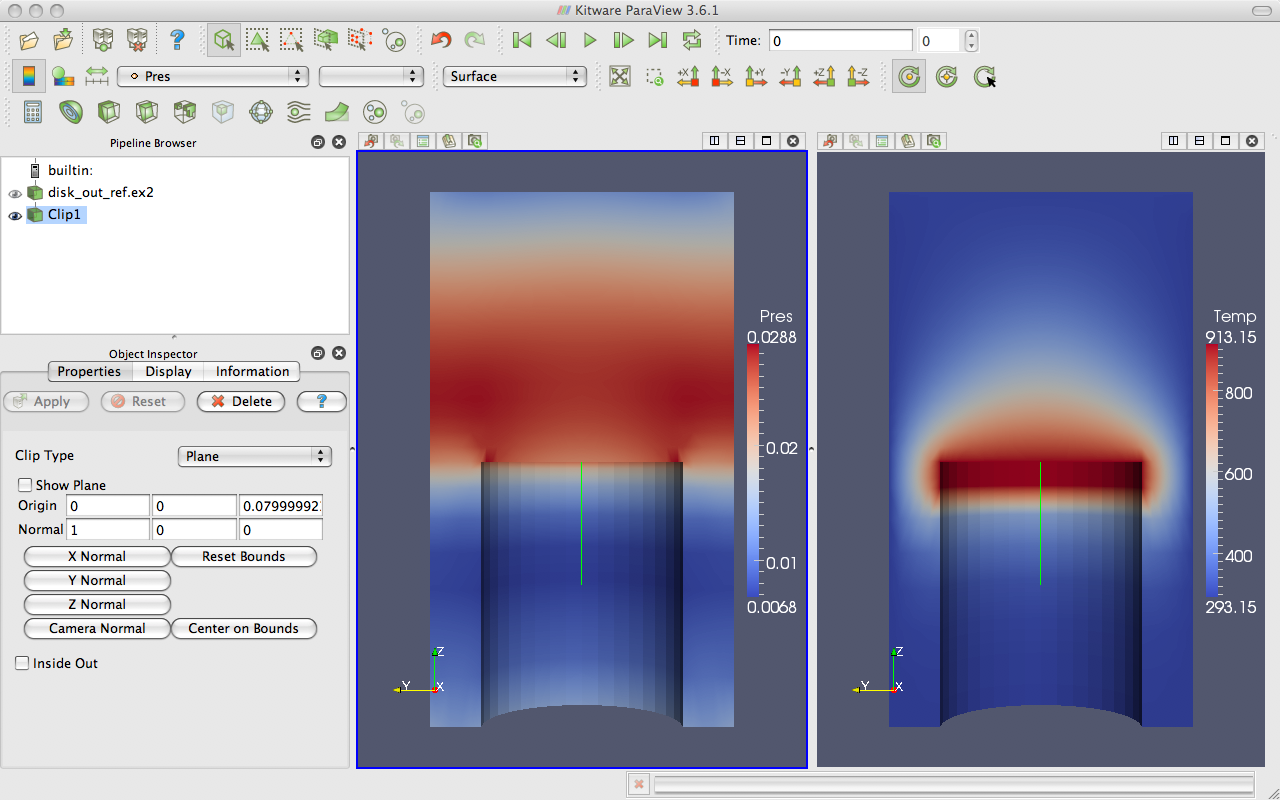
\includegraphics[width=3in]{images/CameraLink}
  \end{inlinefig}

  Notice that the temperature is highest at the interface with the heated
  disk.  That alone is not surprising.  We expect the air temperature to be
  greatest near the heat source and drop off away from it.  But notice that
  at the same position the pressure is not maximal.  The air pressure is
  maximal at a position above the disk.  Based on this information we can
  draw some interesting hypotheses about the physical phenomenon.  We can
  expect that there are two forces contributing to air pressure.  The first
  force is that of gravity causing the upper air to press down on the lower
  air.  The second force is that of the heated air becoming less dense and
  therefore rising.  We can see based on the maximal pressure where these
  two forces are equal.  Such an observation cannot be drawn without
  looking at both the temperature and pressure in this way.
\end{exercise}

Multiview in ParaView is of course not limited to simply two windows.  Note
that each of the views has its own set of multiview buttons.  You can
create more views by using the split view buttons \splitViewH \splitViewV
to arbitrarily divide up the working space.  And you can delete views
\deleteView at any time.

The location of each view is also not fixed.  You are also able to swap two
views by clicking on one of the view toolbars (somewhere outside of where
the buttons are), holding down the mouse button, and dragging onto one of
the other views.  This will immediately swap the two views.

\begin{inlinefig}
  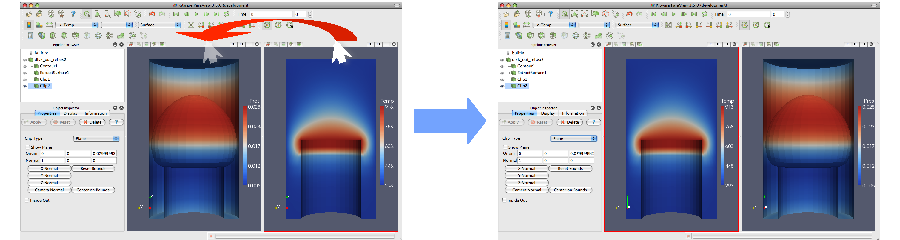
\includegraphics[width=\linewidth]{images/SwapViews}
\end{inlinefig}

You can also change the size of the views by clicking on the space in
between views, holding down the mouse button, and dragging in the direction
of either one of the views.  The divider will follow the mouse and adjust
the size of the views as it moves.

\begin{inlinefig}
  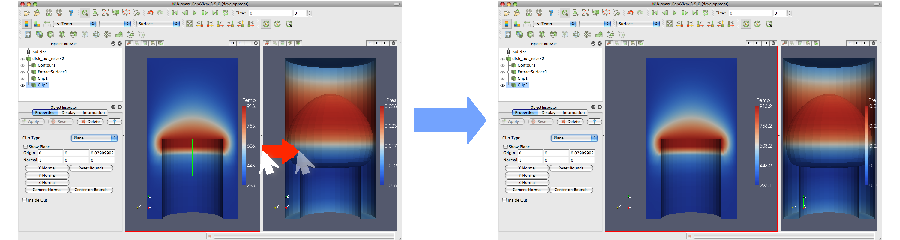
\includegraphics[width=\linewidth]{images/ResizeViews}
\end{inlinefig}


\section{Vector Visualization}

Let us see what else we can learn about this simulation.  The simulation
has also outputted a velocity field describing the movement of the air over
the heated rotating disk.  We will use ParaView to determine the currents
in the air.

A common and effective way to characterize a vector field is with
\keyterm{streamlines}.  A streamline is a curve through space that at every
point is tangent to the vector field.  The represent the path a weightless
particle will take through the vector field (assuming steady-state flow).
Streamlines are generated by providing a set of
\index{stream tracer!seed points} \keyterm{seed points}.

\begin{exercise}{Streamlines}
  \label{ex:Streamlines}%
  We are going to start a fresh visualization, so if you have been
  following along with the exercises so far, now is a good time to reset
  ParaView.  The easiest way to do this is to press the~\disconnect button.

  \begin{enumerate}
  \item Open the file disk\_out\_ref.ex2, load all variables, \apply (see
    Exercise~\ref{ex:OpeningAFile}).
  \item Add the stream tracer filter \streamTracer to
    \gui{disk\_out\_ref.ex2}.
  \item Click the \apply button to accept the default parameters.
  \end{enumerate}

  \begin{inlinefig}
    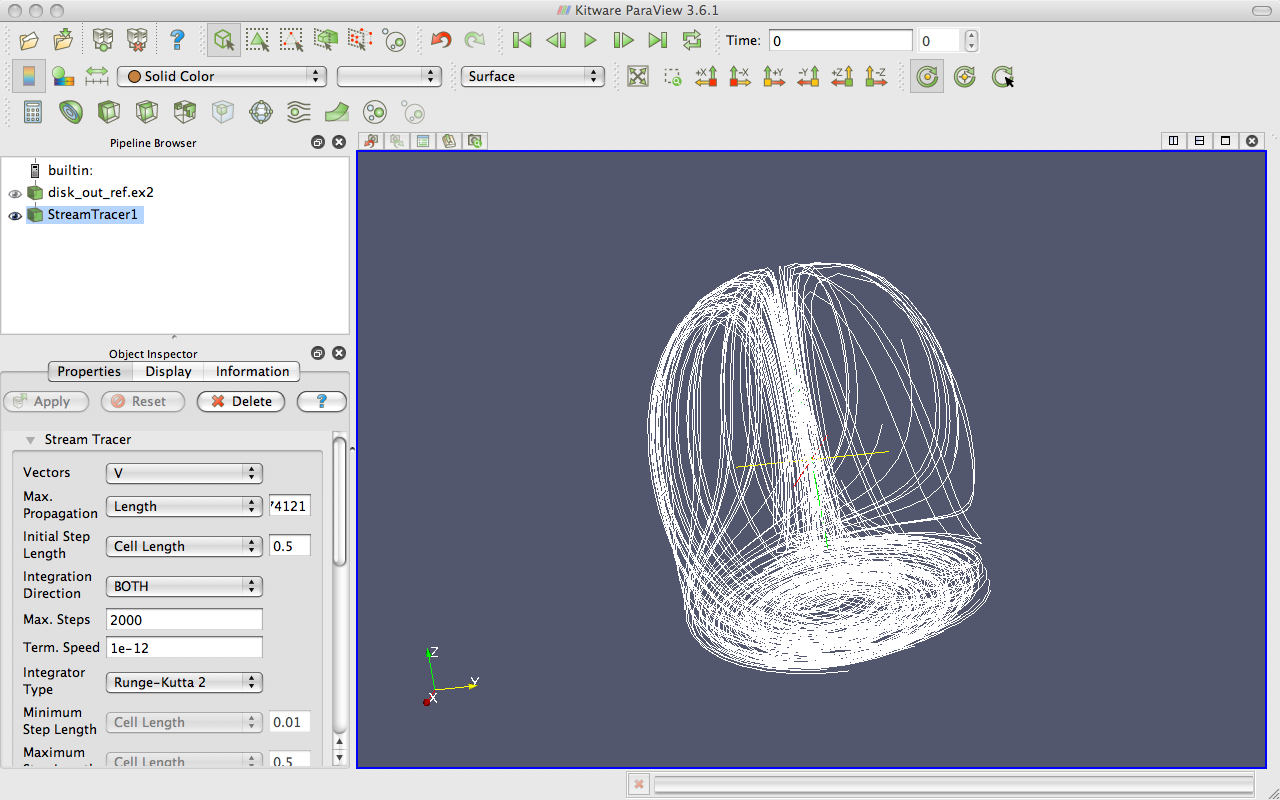
\includegraphics[width=3in]{images/StreamTracer0}
  \end{inlinefig}

  The surface of the mesh is replaced with some swirling lines.  These
  lines represent the flow through the volume.  Notice that there is a
  spinning motion around the center line of the cylinder.  There is also a
  vertical motion in the center and near the edges.

  The new geometry is off-center from the previous geometry.  We can
  quickly center the view on the new geometry with the \keyterm{reset
    camera}~\resetCamera command.  This command centers and fits the
  visible geometry within the current view and also resets the center of
  rotation to the middle of the visible geometry.
\end{exercise}

One issue with the streamlines as they stand now is that the lines are
difficult to distinguish because there are many close together and they
have no shading.  Lines are a 1D structure and shading requires a 2D
surface.  Another issue with the streamlines is that we cannot be sure in which
direction to flow is.

In the next exercise, we will modify the streamlines we created in
Exercise~\ref{ex:Streamlines} to correct these problems.  We can create a
2D surface around our stream traces with the tube filter.  This surface
adds shading and depth cues to the lines.  We can also add glyphs to the
lines that point in the direction of the flow.

\begin{exercise}{Making Streamlines Fancy}
  \label{ex:MakingStreamlinesFancy}%
  \begin{enumerate}
  \item Use the quick launch (ctrl+space Win/Linux, alt+space Mac) to apply
    the \gui{Tube}\index{tube} filter.\footnote{In ParaView 3.6 the name of
      the tube filter was changed to \index{generate tubes}\gui{Generate
        Tubes}.  In future versions, the name will change back to
      \gui{Tube} to make it easier to find in alphabetical filter lists.}
  \item Hit the \apply button.
    \savecounter
  \end{enumerate}

  \begin{inlinefig}
    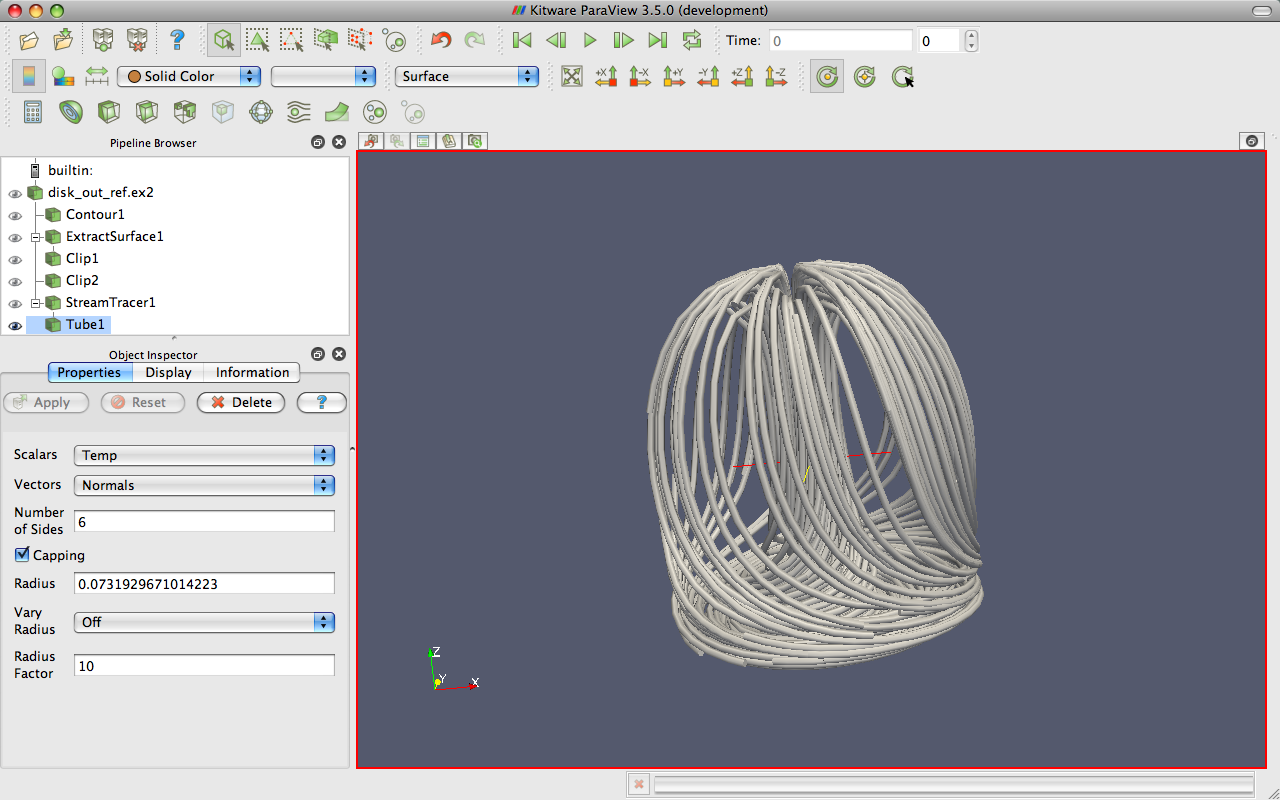
\includegraphics[width=3in]{images/StreamTracer1}
  \end{inlinefig}

  You can now see the streamlines much more clearly.  As you look at the
  streamlines from the side, you should be able to see circular convection
  as air heats, rises, cools, and falls.  If you rotate the streams to look
  down the Z axis at the bottom near where the heated plate should be, you
  will also see that the air is moving in a circular pattern due to the
  friction of the rotating disk.

  Now we can get a little fancier.  We can add glyphs to the streamlines to
  show the orientation and magnitude.

  \begin{enumerate}
    \restorecounter
  \item Select \gui{StreamTracer1} in the pipeline browser.
  \item Add the glyph filter~\glyph to \gui{StreamTracer1}.
  \item In the object inspector, change the \gui{Vectors} option (second
    option from the top) to \gui{V}.
  \item In the object inspector, change the \gui{Glyph Type} option (third
    option from the top) to \gui{Cone}.
  \item Hit the \apply button.
  \item Color the glyphs with the \gui{Temp} variable.
  \end{enumerate}

  \begin{inlinefig}
    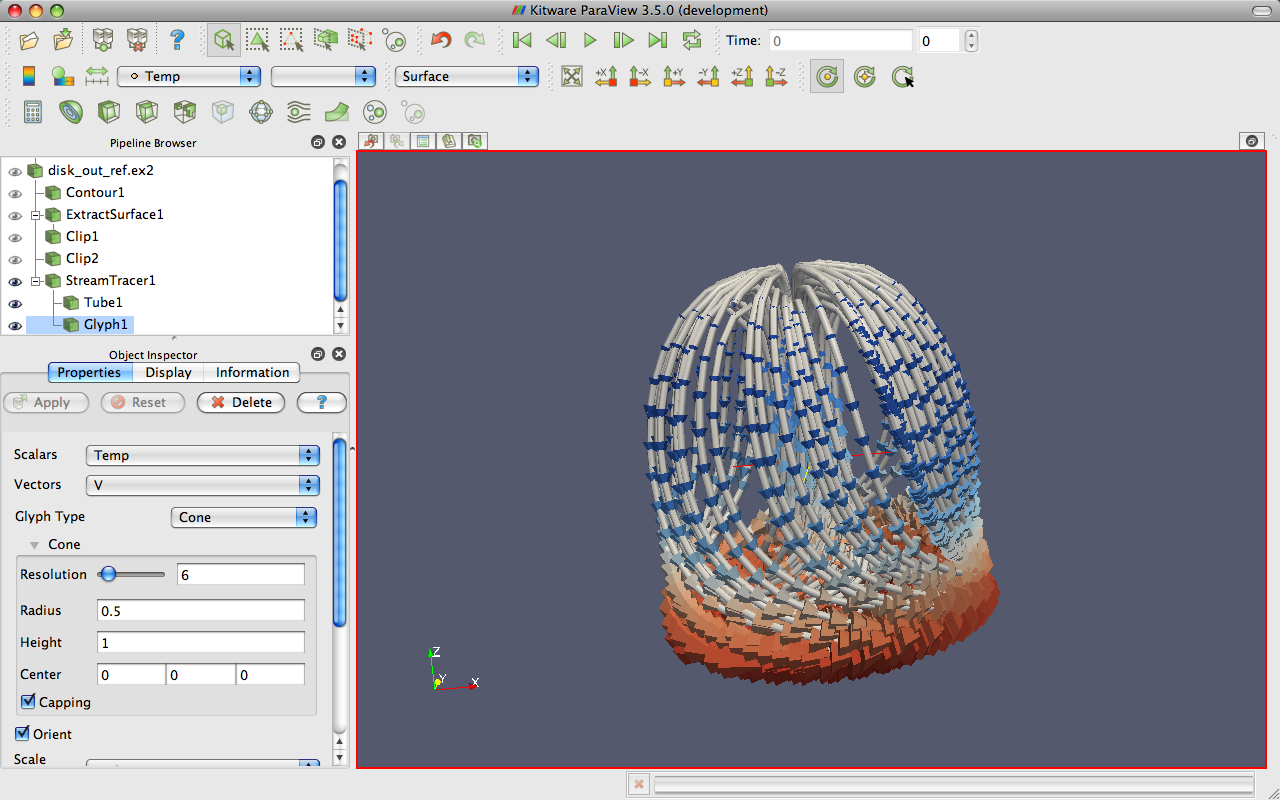
\includegraphics[width=3in]{images/StreamTracer2}
  \end{inlinefig}

  Now the streamlines are augmented with little pointers.  The pointers
  face in the direction of the velocity, and their size is proportional to
  the magnitude of the velocity.  Try using this new information to answer
  the following questions.

  \begin{itemize}
  \item Where is the air moving the fastest?  Near the disk or away from it?
    At the center of the disk or near its edges?
  \item Which way is the plate spinning?
  \item At the surface of the disk, is air moving toward the center or away
    from it?
  \end{itemize}
\end{exercise}


\section{Plotting}

ParaView's plotting capabilities provide a mechanism to drill down into
your data to allow quantitative analysis.  Plots are usually created with
filters, and all of the plotting filters can be found in the \gui{Data
  Analysis} submenu of \gui{Filters}.  In the next exercise, we create a
filter that will plot the values of the mesh’s fields over a line in space.

\begin{exercise}{Plot Over a Line in Space}
  \label{ex:PlotOverLine}%
  We are going to start a fresh visualization, so if you have been
  following along with the exercises so far, now is a good time to reset
  ParaView.  The easiest way to do this is to press the~\disconnect button.

  \begin{enumerate}
  \item Open the file disk\_out\_ref.ex2, load all variables, \apply (see
    Exercise~\ref{ex:OpeningAFile}).
  \item Add the Clip filter~\clip to \gui{disk\_out\_ref.ex2}, Uncheck the
    Show Plane checkbox \includeinlinegraphics{images/ShowPlaneCheckbox} in
    the object inspector, and click \apply (like in
    Exercise~\ref{ex:UsingMultipleViews}).  This will make it easier to see
    and manipulate the line we are plotting over.
  \item Click on \gui{disk\_out\_ref.ex2} in the pipeline browser to make
    that the active object.
  \item From the menu bar, select \gui{Filters} \ra \gui{Data Analysis} \ra
    \gui{Plot Over Line}~\icon{pqPlotLineOverTime24} or apply the \gui{Plot
      Over Line} filter using the quick launch (ctrl+space Win/Linux,
    alt+space Mac). \index{plot~over~line} \savecounter
  \end{enumerate}

  \begin{inlinefig}
    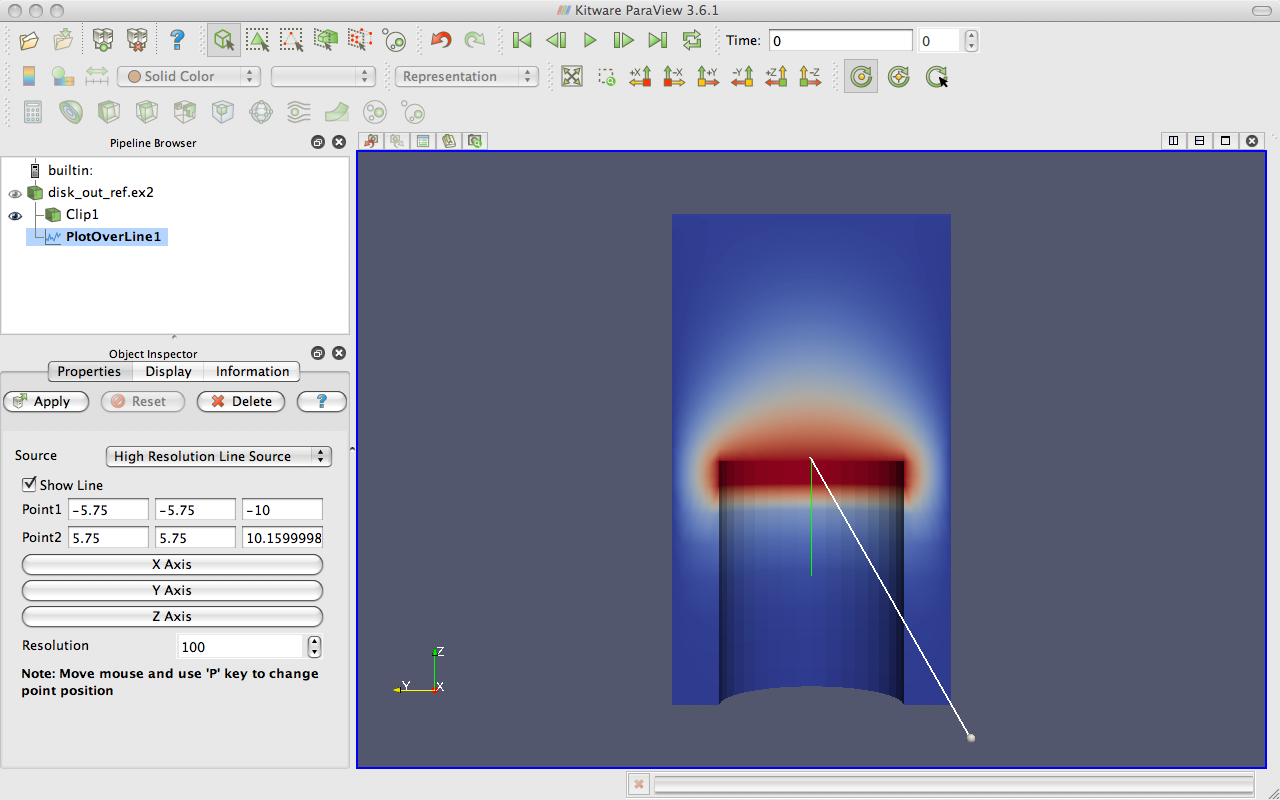
\includegraphics[width=3in]{images/LinePlot1}
  \end{inlinefig}

  In the active view you will see a line through your data with a ball at
  each end.  If you move your mouse over either of these balls, you can
  drag the balls through the 3D view to place them.  Notice that each time
  you move the balls some of the fields in the object inspector also
  change.  You can also place the balls by hovering your mouse over the
  target location and hitting the p key.  This will alternatively place
  each ball at the surface underneath the mouse cursor.  This was the
  purpose of adding the clip filter: It allows us to easily add the
  endpoints to this plane.  Note that placing the endpoints in this manner
  only works when rendering solid surfaces.  It will not work with a volume
  rendered image.

  This representation is called a \keyterm{3D widget} because it is a GUI
  component that is manipulated in 3D space.  There are many examples of 3D
  widgets in ParaView.  This particular widget, the line widget, allows you
  to specify a line segment in space.  Other widgets allow you to specify
  points or planes.

  \begin{enumerate}
    \restorecounter
  \item Adjust the line so that it goes from the base of the disk straight up
    to the top of the mesh using the 3D widget manipulators, the p key
    shortcut, or the object inspector parameters.
  \item Once you have your line satisfactorily located, click the \apply
    button.
  \end{enumerate}

  \begin{inlinefig}
    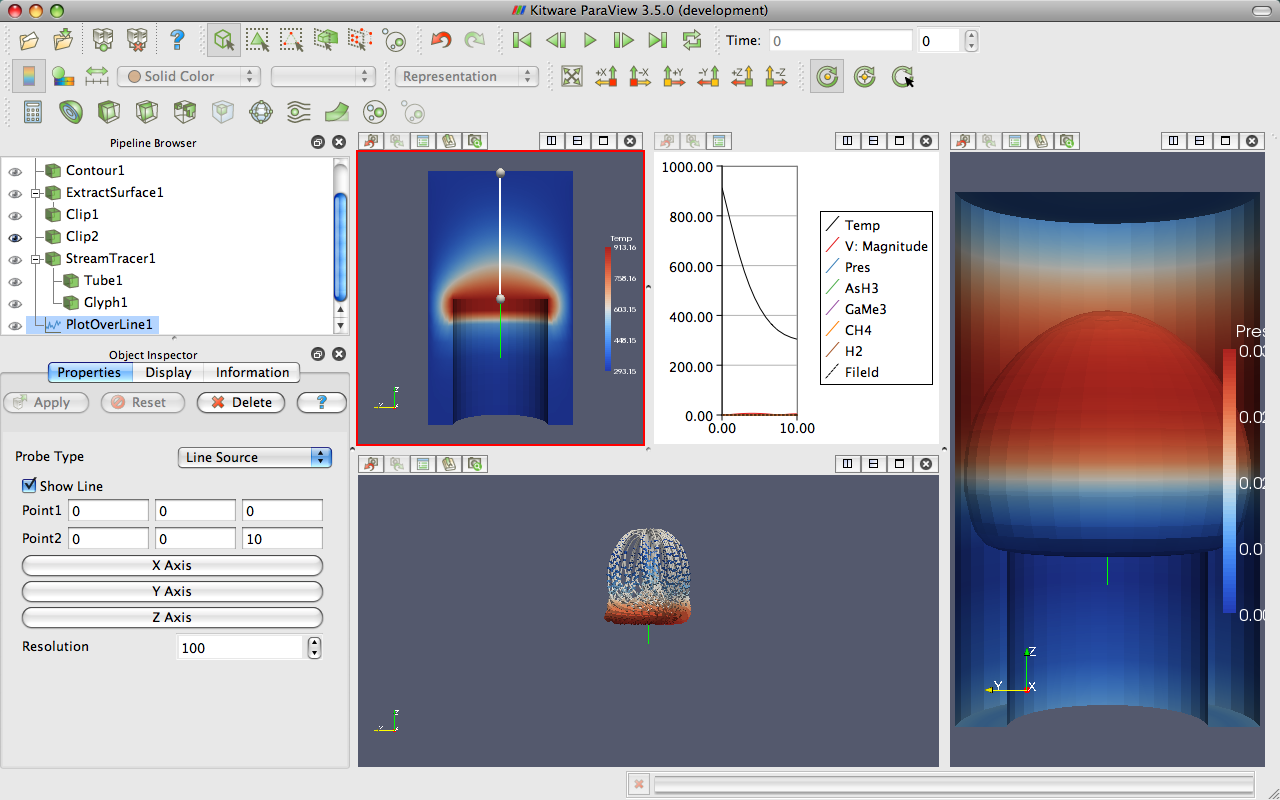
\includegraphics[width=3in]{images/LinePlot2}
  \end{inlinefig}

  There are several interactions you can do with the plot.  Drag with the
  middle button up and down to zoom in and out.  Drag with the right button
  to do a rubber band zoom.  Drag with the left button to scroll the plot
  around.  You can also use the reset camera command~\resetCamera to restore
  the view to the full domain and range of the plot.
\end{exercise}

Plots, like 3D renderings, are considered views.  Both provide a
representation for your data; they just do it in different ways.  Because
plots are views, you interact with them in much the same ways as with a 3D
view.  If you look in the \gui{Display} tab of the object inspector, you
will see many options on the representation for each line of the plot
including colors, line styles, vector components, and legend names.
\begin{inlinefig}
  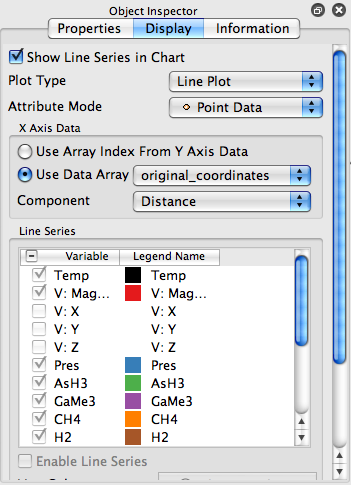
\includegraphics[width=1.5in]{images/PlotDisplayTab}
\end{inlinefig}

Plots also have a \icon{pqOptions16} button that brings up a dialog that
allows you to change plot-wide options such as labels, legends, and axes
ranges.
\begin{inlinefig}
  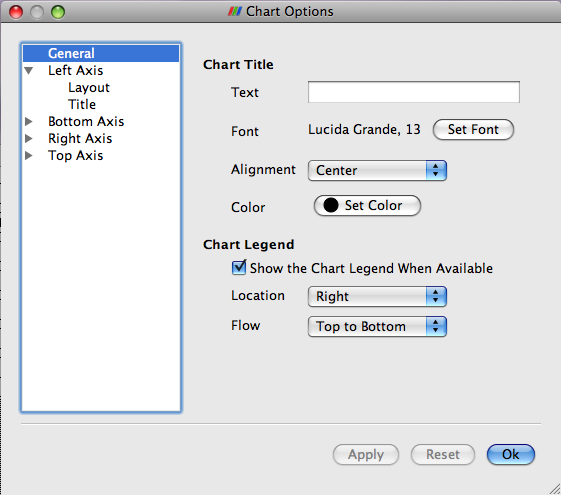
\includegraphics[width=2in]{images/PlotViewOptions}
\end{inlinefig}

Like any other views, you can capture the plot with the \gui{File} \ra
\icon{pqCaptureScreenshot24}~\gui{Save Screenshot}.  As an added bonus, you
can save can save the plot in a vector PDF format so that it scales well if
included in reports and other documents.  You can also move around plots in
the GUI like you can other views.

In the next exercise, we use these features to get more information out of
our plot.  Specifically, we use the plot to compare the pressure and
temperature variables.

\begin{exercise}{Plot Series Display Options}
  \label{ex:PlotSeriesDisplayOptions}%
  This exercise is a continuation of Exercise~\ref{ex:PlotOverLine}.  You
  will need to finish that exercise before beginning this one.

  \begin{enumerate}
  \item Choose a place in your GUI that you would like the plot to go and
    try using the split, delete, resize, and swap view features to move it
    there.
  \item Make the plot view active, go to the \gui{Display} tab, and turn
    off all variables except \gui{Temp} and \gui{Pres}.
    \savecounter
  \end{enumerate}

  The \gui{Temp} and \gui{Pres} variables have different units.  Putting
  them on the same scale is not useful.  We can still compare them in the
  same plot by placing each variable on its own scale.  The line plot in
  ParaView allows for a different scale on the left and right axis, and you
  can scale each variable individually on each axis.

  \begin{enumerate}
    \restorecounter
  \item Select the \gui{Pres} variable in the \gui{Display} tab.
  \item Change the \gui{Chart Axis} to \gui{Bottom - Right}
  \end{enumerate}

  \begin{inlinefig}
    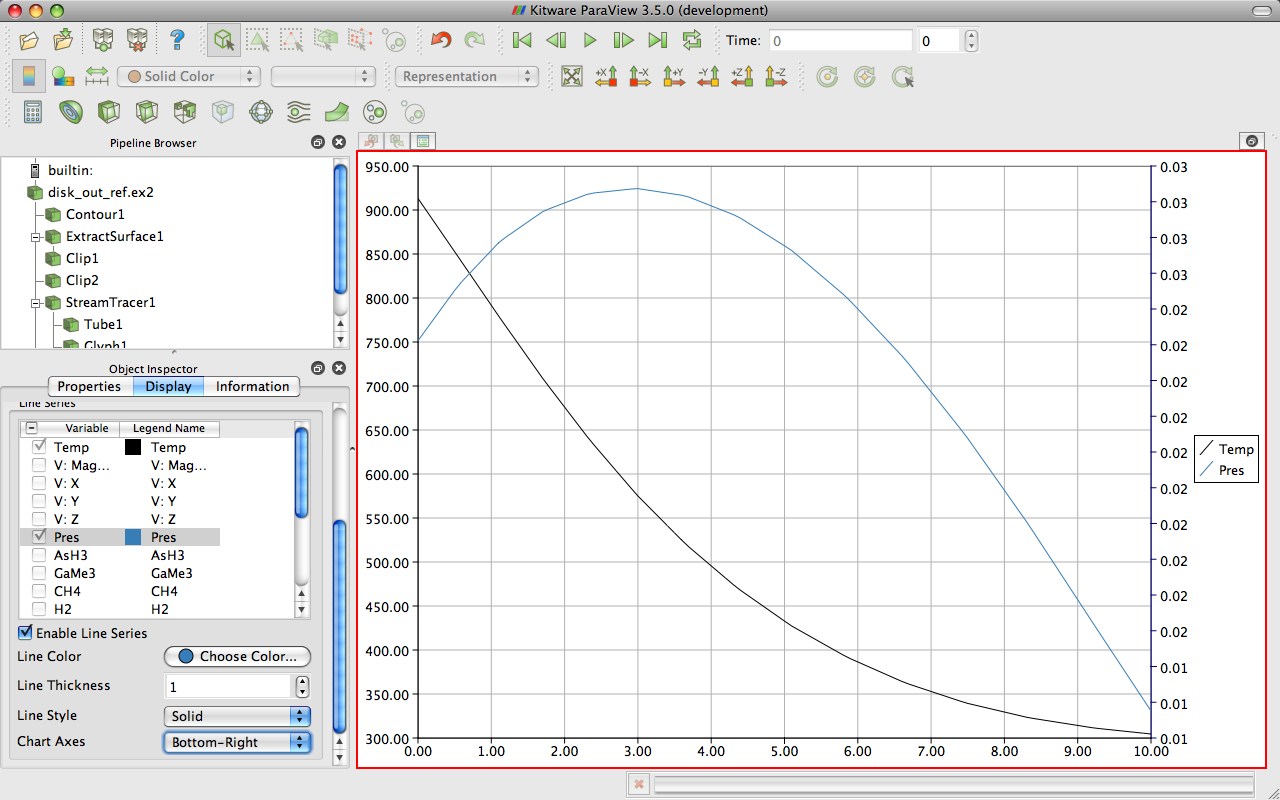
\includegraphics[width=3in]{images/LinePlot3}
  \end{inlinefig}

  From this plot we can verify some of the observations we made in
  Section~\ref{sec:Multiview}.  We can see that the temperature is maximal
  at the plate surface and falls as we move away from the plate, but the
  pressure goes up and then back down.  In addition, we can observe that
  the maximal pressure (and hence the location where the forces on the air
  are equalized) is three units away from the disk.
\end{exercise}

The ParaView framework is designed to accommodate any number of different
types of views.  This is to provide researchers and developers a way to
deliver new ways of looking at data.  To see another example of view,
select \gui{disk\_out\_ref.ex2} in the pipeline browser, and then select
\gui{Filters} \ra \gui{Data Analysis} \ra
\gui{Histogram}~\icon{pqHistogram24}. \index{histogram} Make the histogram
for the Temp variable, and then hit the \apply button.

\begin{inlinefig}
  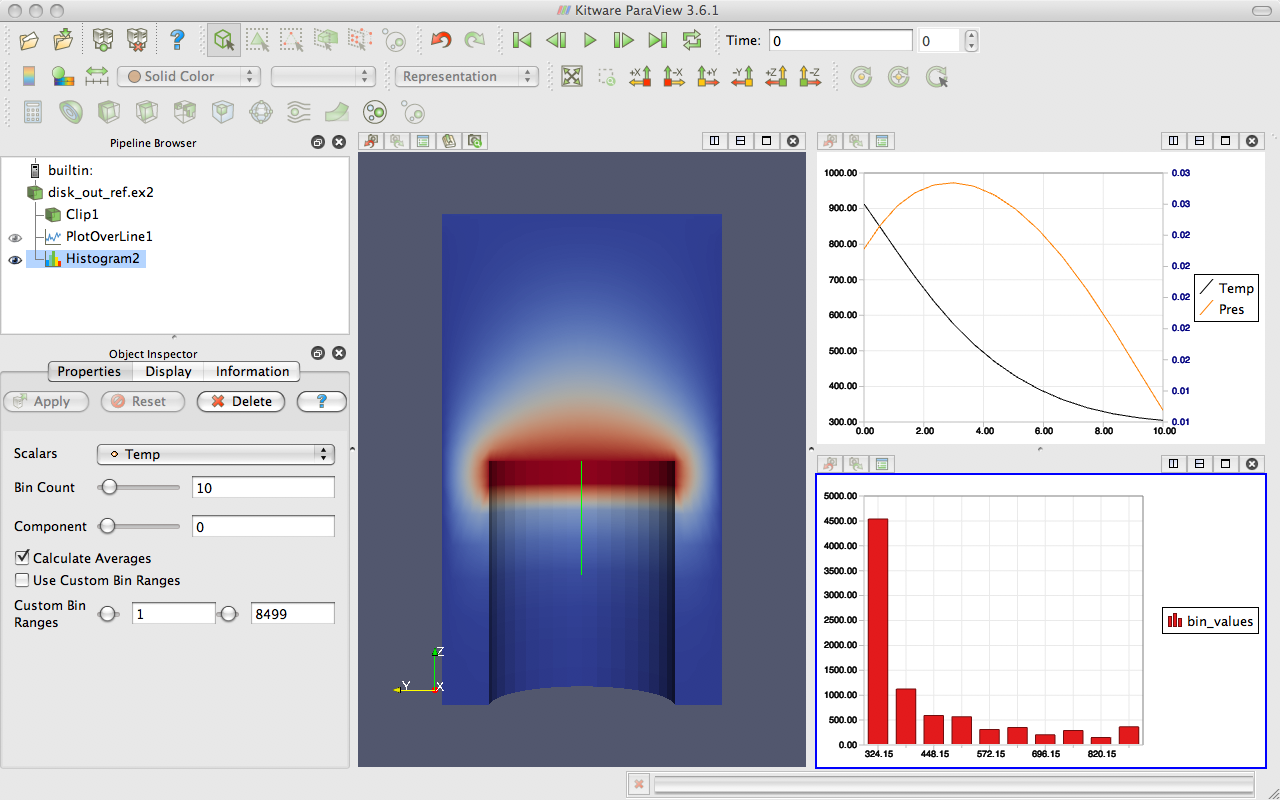
\includegraphics[width=3in]{images/HistogramPlot}
\end{inlinefig}


\section{Volume Rendering}

ParaView has several ways to represent data.  We have already seen some
examples: surfaces, wireframe, and a combination of both.  ParaView can
also render the points on the surface or simply draw a bounding box of the
data.

\begin{inlinefig}
  \begin{tabular}{c@{\;}c@{\;}c@{\;}c@{\;}c}
    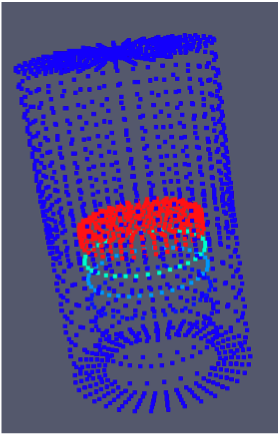
\includegraphics[width=.18\linewidth]{images/RepresentationPoints} &
    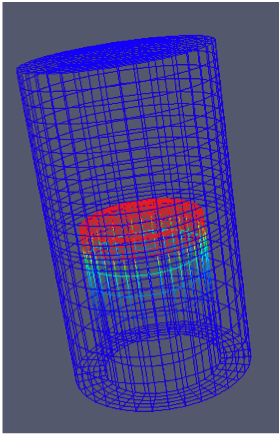
\includegraphics[width=.18\linewidth]{images/RepresentationWireframe} &
    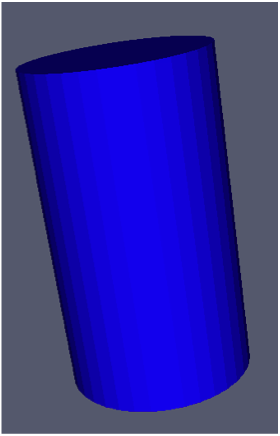
\includegraphics[width=.18\linewidth]{images/RepresentationSurface} &
    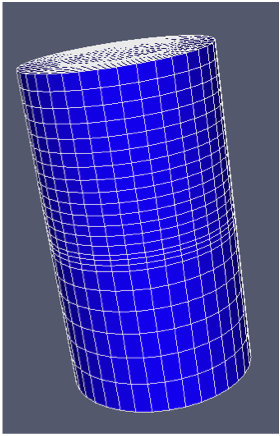
\includegraphics[width=.18\linewidth]{images/RepresentationSurfaceEdges} &
    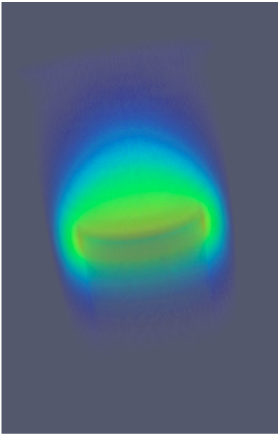
\includegraphics[width=.18\linewidth]{images/RepresentationVolume}
    \\
    Points &
    Wireframe &
    Surface &
    \parbox[t]{.18\linewidth}{\centering{}Surface with Edges} &
    Volume
  \end{tabular}
\end{inlinefig}

A powerful way that ParaView lets you represent your data is with a
technique called \keyterm{volume rendering}.  With volume rendering, a
solid mesh is rendered as a translucent cloud with the scalar field
determining the color and density at every point in the cloud.  Unlike with
surface rendering, volume rendering allows you to see features all the way
through a volume.

Volume rendering is enabled by simply changing the representation of the
object.  Let us try an example of that now.

\begin{exercise}{Turning On Volume Rendering}
  \label{ex:VolumeRendering}%
  We are going to start a fresh visualization, so if you have been
  following along with the exercises so far, now is a good time to reset
  ParaView.  The easiest way to do this is to press the~\disconnect button.

  \begin{enumerate}
  \item Open the file disk\_out\_ref.ex2, load all variables, \apply (see
    Exercise~\ref{ex:OpeningAFile}).
  \item Make sure \gui{disk\_out\_ref.ex2} is selected in the pipeline
    browser.  Change the variable viewed to \gui{Temp} and change the
    representation to \gui{Volume}.
  \end{enumerate}

  \begin{inlinefig}
    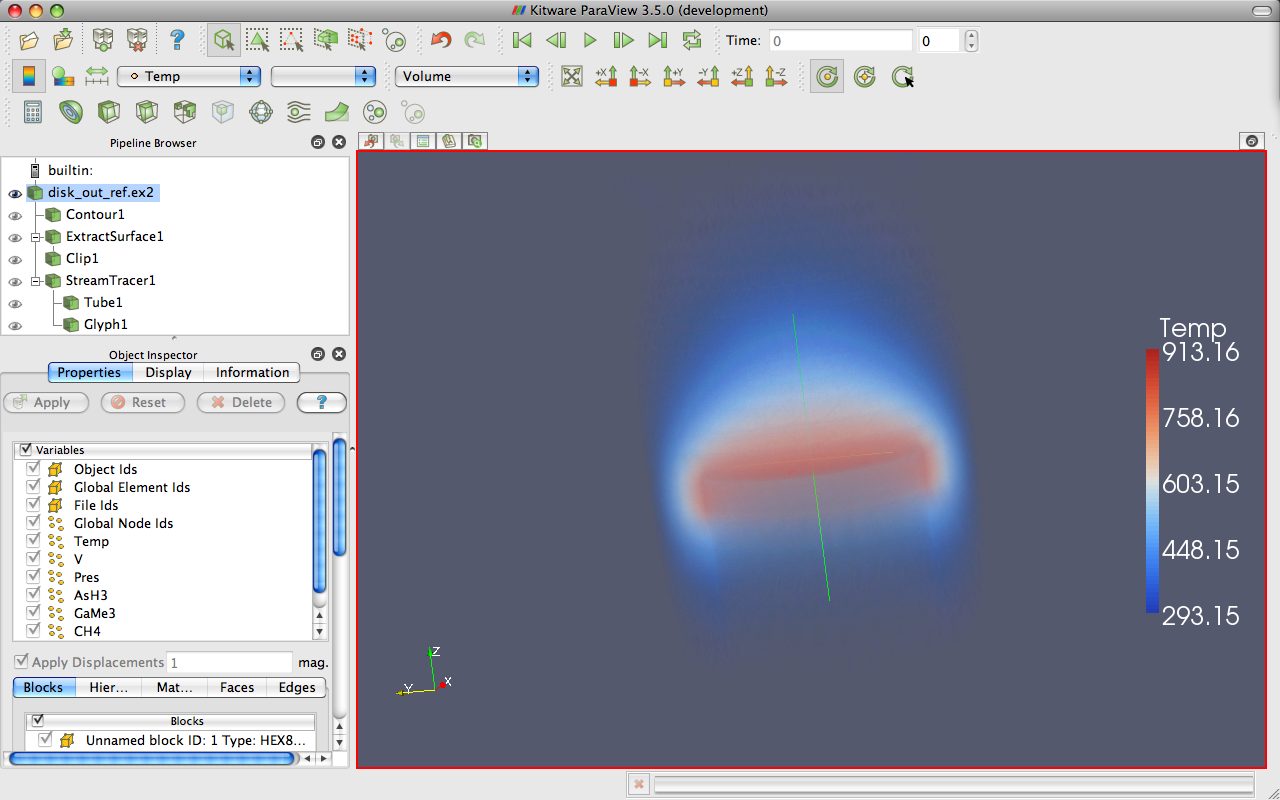
\includegraphics[width=3in]{images/VolumeRender1}
  \end{inlinefig}

  The solid opaque mesh is replaced with a translucent volume. You may
  notice that when rotating the image is temporarily replaced with a
  simpler image for performance reasons, which we will discuss this feature
  in more detail later in Chapter~\ref{chap:VisualizingLargeModels}.
\end{exercise}

A useful feature of ParaView’s volume rendering is that it can be mixed
with the surface rendering of other objects.  This allows you to add
context to the volume rendering or to mix visualizations for a more
information-rich view.  For example, we can combine this volume rendering
with a streamline vector visualization like we did in
Exercise~\ref{ex:Streamlines}.

\begin{exercise}{Combining Volume Rendering and Surface-Based Visualization}
  \label{ex:CombiningVolumeAndSurfaceRendering}%
  This exercise is a continuation of Exercise~\ref{ex:VolumeRendering}.
  You will need to finish that exercise before beginning this one.

  \begin{enumerate}
  \item Add the stream tracer filter \streamTracer to
    \gui{disk\_out\_ref.ex2}.
  \item Click the \apply button to accept the default parameters.
    \savecounter
  \end{enumerate}

  You should now be seeing the streamlines embedded within the volume
  rendering.  The following additional steps add geometry to make the
  streamlines easier to see much like in
  Exercise~\ref{ex:MakingStreamlinesFancy}.  They are optional, so you can
  skip them if you wish.

  \begin{enumerate}
    \restorecounter
  \item Use the quick launch (ctrl+space Win/Linux, alt+space Mac) to apply
    the \gui{Tube}\index{tube} filter and hit \apply.
  \item If the streamlines are colored by \gui{Temp}, change that to
    \gui{Solid Color}.
  \item Select \gui{StreamTracer1} in the pipeline browser.
  \item Add the glyph filter~\glyph to \gui{StreamTracer1}.
  \item In the object inspector, change the \gui{Vectors} option (second
    option from the top) to \gui{V}.
  \item In the object inspector, change the \gui{Glyph Type} option (third
    option from the top) to \gui{Cone}.
  \item Hit the \apply button.
  \item Color the glyphs with the \gui{Temp} variable.
  \end{enumerate}

  \begin{inlinefig}
    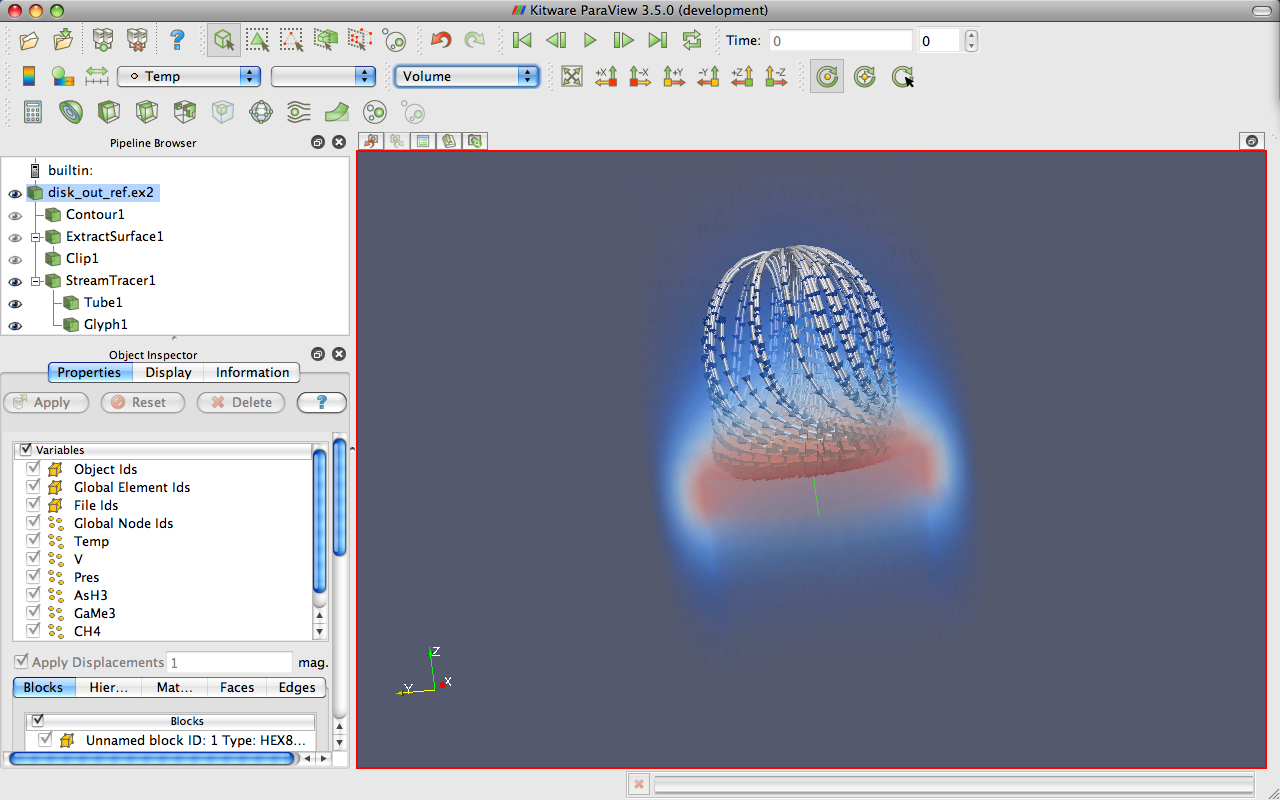
\includegraphics[width=3in]{images/VolumeRender2}
  \end{inlinefig}

  The streamlines are now shown in context with the temperature throughout
  the volume.
\end{exercise}

By default, ParaView will render the volume with the same colors as used on
the surface with the transparency set to 0 for the low end of the range and
1 for the high end of the range.  ParaView also provides an easy way to
change the \keyterm{transfer function}, how scalar values are mapped to
color and transparency.  You can access the transfer function editor by
selecting the volume rendered pipeline object and clicking on the edit
color map~\icon{pqEditColor24} button.

\begin{inlinefig}
  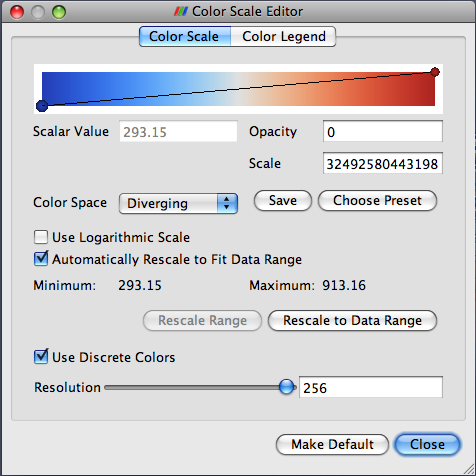
\includegraphics[width=2.5in]{images/ColorScaleEditor}
\end{inlinefig}

The resulting dialog box provides options for editing the transfer
function.  The colorful box at top displays the colors of the transfer
function with a plot of the transparency in black.  The dots on the
transfer function represent the \keyterm{control points}.  The control
points are the specific color and opacity you set at particular scalar
values, and the colors and transparency are interpolated between them.
Clicking on a blank spot in the bar will create a new control point.
Clicking on an existing control point will select it.  The selected control
point can be dragged throughout the box to change its scalar value and
transparency, and clicking again on the selected control point will bring
up a dialog box.  The selected control point will be deleted when you hit
the backspace or delete key.

Directly below the color bar are text entry widgets to numerically specify
the \gui{Scalar Value} or \gui{Opacity} of the selected control point.  The
Scale parameter adjusts the unit length of the opacity calculation.  Larger
numbers make the volume less opaque.  The \gui{Color Space} parameter
changes how colors are interpolated.  This parameter has no effect on the
color at the control points, but can drastically affect the colors between
the control points.  You can also change to a logarithmic scaling of colors
via the \gui{Use Logarithmic Scale} checkbox.

Setting up a transfer function can be tedious, so you can save it by
clicking the \includeinlinegraphics{images/ColorMapSave} button.  The
\includeinlinegraphics{images/ColorMapChoosePreset} button brings up a
dialog that allows you to manage and apply the color maps that you have
created as well as several provided by ParaView.

\begin{exercise}{Modifying Volume Rendering Transfer Functions}
  \label{ex:ModifyingVolumeRenderingTransferFunctions}%
  This exercise is a continuation of
  Exercise~\ref{ex:CombiningVolumeAndSurfaceRendering}.  You will need to
  finish that exercise (or minimally Exercise~\ref{ex:VolumeRendering})
  before beginning this one.

  \begin{enumerate}
  \item Click on \gui{disk\_out\_ref.ex2} in the pipeline browser to make
    that the active object.
  \item Click on the edit color map~\icon{pqEditColor24} button.
  \item Try adding and changing control points and observe their effect on
    the volume rendering.
  \item Change the volume rendering to be more representative of heat.
    Press \includeinlinegraphics{images/ColorMapChoosePreset}, select
    \gui{Black-Body Radiation} in the dialog box, and then click \gui{OK}.
  \end{enumerate}

  \begin{inlinefig}
    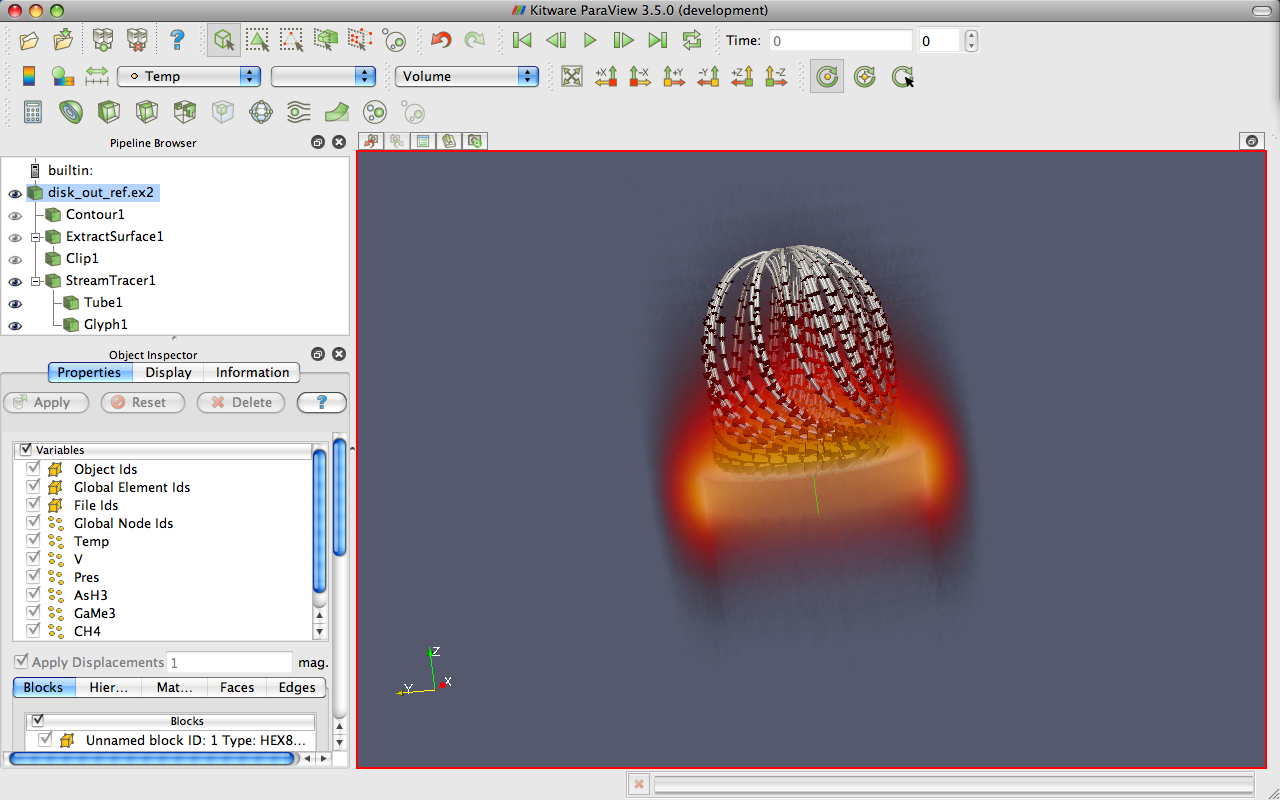
\includegraphics[width=3in]{images/VolumeRender3}
  \end{inlinefig}

  Notice that not only did the color mapping in the volume rendering
  change, but all the color mapping for \gui{Temp} changed.  This ensures
  consistency between the views and avoids any confusion from mapping the
  same variable with different colors or different ranges.
\end{exercise}


\section{Time}

Now that we have thoroughly analyzed the disk\_out\_ref simulation, we will
move to a new simulation to see how ParaView handles time.  In this section
we will use a new data set from another simple simulation, this time with
data that changes over time.

\begin{exercise}{Loading Temporal Data}
  \label{ex:LoadingTemporalData}%
  We are going to start a fresh visualization, so if you have been
  following along with the exercises so far, now is a good time to reset
  ParaView.  The easiest way to do this is to press the~\disconnect button.

  \begin{enumerate}
  \item \gui{Open} the file \gui{can.ex2}.
    \begin{inlinefig}
      \includegraphics{images/Variables_can}
    \end{inlinefig}
  \item As before, click the checkbox in the header of the variable list to
    turn on the loading of all the variables and hit the \apply button.
  \item Press the~\yPlus button to orient the camera to the mesh.
  \item Press the play button~\vcrPlay in the toolbars and watch ParaView
    animate the mesh to crush the can with the falling brick.
  \end{enumerate}

  \begin{inlinefig}
    \includegraphics[width=.32\linewidth]{images/AnimateCan1}
    \includegraphics[width=.32\linewidth]{images/AnimateCan2}
    \includegraphics[width=.32\linewidth]{images/AnimateCan3}
  \end{inlinefig}
\end{exercise}

That is really all there is to dealing with data that is defined over time.
ParaView has an internal concept of time and automatically links in the
time defined by your data.  Become familiar with the toolbars that can be
used to control time.

\begin{inlinefig}
  \includegraphics[width=\linewidth]{images/AnimationToolbar}
\end{inlinefig}

Saving an animation is equally as easy.  From the menu, select \gui{File}
\ra \gui{Save Animation}.  ParaView provides dialogs specifying how you
want to save the animation, and then automatically iterates and saves the
animation.

\begin{exercise}{Temporal Data Pitfall}
  \label{ex:TemporalDataPitfall}%
  The biggest pitfall users run into is that with mapping a set of colors
  whose range changes over time.  To demonstrate this, do the following.

  \begin{enumerate}
  \item If you are not continuing from
    Exercise~\ref{ex:LoadingTemporalData}, open the file \gui{can.ex2},
    load all variables, \apply.
  \item Go to the first time step~\vcrFirst.
  \item Turn on the \gui{EQPS} variable.
  \item Turn on the color legend~\icon{pqScalarBar32}.
  \item Play~\vcrPlay through the animation (or skip to the last time
    step~\vcrLast).
    \savecounter
  \end{enumerate}

  The coloring is not very useful.  To quickly fix the problem:

  \begin{enumerate}
    \restorecounter
  \item While at the last time step, click the Rescale to Data
    Range~\icon{pqResetRange24} button.
  \item Play~\vcrPlay the animation again.
  \end{enumerate}

  The colors are more useful now.
\end{exercise}

Although this behavior seems like a bug, it is not.  It is the consequence
of two unavoidable behaviors.  First, when you turn on the visibility of a
scalar field, the range of the field is set to the range of values in the
current time step.  Ideally, the range would be set to the max and min over
all time steps in the data.  However, that would require ParaView to load
in all of the data on the initial read, and that would be prohibitively
slow for large data.  Second, when you animate over time, it is important
to hold the color range fixed even if the range in the data changes.
Changing the scale of the data as an animation plays causes a
misrepresentation of the data.  It is far better to let the scalars go out
of the original color maps range than to imply that they have not.  To get
around the problem, simply go to a representative time step and
hit~\icon{pqResetRange24} or open the edit color scale dialog
box~\icon{pqEditColor24} and specify a range for the data.


\section{Selection}

A feature that greatly improved with the release of ParaView 3 and
continues to evolve is that of selection.  Selection can take place at any
time, and ParaView maintains a current selected set that is linked between
all views.  That is, if you select something in one view, that selection is
also shown in all other views that display the same object.

ParaView allows you to select points, cells, or blocks of a single data
set.  There are also multiple ways of specifying the elements to include in
the selection including id lists of multiple varieties, spatial locations,
and scalar values.  We will explore some of the combinations now.

One of the easiest ways of creating a selection is to pick elements right
inside the 3D view.  All of the 3D view selections are performed with a
\keyterm{rubber-band} selection.  That is, by clicking and dragging the
mouse in the 3D view, you will create a boxed region that will select
elements underneath it.  There are several types of rubber-band selection
that can be performed, and you initiate one by selecting one of the icons
in the selection controls toolbar or using one of the shortcut keys.  The
following 3D selections are possible.

\begin{description}
\item[\selectCellsOn Select Cells On (Surface)] Selects cells that are
  visible in the view.  (Shortcut: s)
\item[\selectPointsOn Select Points On (Surface)] Selects points that are
  visible in the view.
\item[\selectCellsThrough Select Cells Through (Frustum)] Selects all cells
  that exist under the rubber band.
\item[\selectPointsThrough Select Points Through (Frustum)] Selects all
  points that exist under the rubber band.
\item[\selectBlocks Select Blocks] Selects blocks in a
  multiblock data set.  (Shortcut: b)
\end{description}

The shortcuts s and b allow you to quickly select a cell or block,
respectively.  Use them by placing the mouse cursor somewhere in the
currently selected 3D view and hitting the appropriate key.  Then click on
the cell or block you want selected (or drag a rubber band over multiple
elements).

Feel free to experiment with the selections now.

\begin{inlinefig}
  \includegraphics{images/SelectionInspector}
\end{inlinefig}

You can manage your selection with the \keyterm{selection inspector}.  You
can view the selection inspector through the menu \gui{View} \ra
\gui{Selection Inspector}.  The selection inspector allows you to view all
the points and cells in the selection as well as modify the selection.  You
can also use the selection inspector to add labels to the selection to make
it easier to identify which element is which.

Experiment with the selection inspector a bit.  Open the \gui{Selection
  Inspector}.  Then make selections using the rubber-band selection and see
the results in the \gui{Selection Inspector}.  Also experiment with
altering the selection by changing ids or inverting selections with the
\gui{Invert selection} checkbox.

You will notice that the select-on tools, \selectCellsOn/\selectPointsOn,
show a list of points/cells and the select blocks tool,~\selectBlocks,
shows a list of blocks, but the select-through tools,
\selectCellsThrough/\selectPointsThrough show neither.  That is because it
is selecting a region in space.  If you click on the \gui{Show Frustum} and
rotate the 3D view to see the region of the selection.

It should be noted that there is a fundamental difference between
selections that specify a list of points or cells and a selection that
specifies a region in space.  The following exercise demonstrates the
difference.

\begin{exercise}{Data Element Selections vs. Spatial Selections}
  \label{ex:DataElementSelectionsVsSpatialSelections}%

  \begin{enumerate}
  \item If you do not already have it loaded from the previous exercise,
    open the file \gui{can.ex2}, load all variables, \apply (see
    Exercise~\ref{ex:LoadingTemporalData}).
  \item Make a selection using the \gui{Select Cells
    Through}~\selectCellsThrough tool.
  \item Click on the \gui{Show Frustum} checkbox in the \gui{Selection
    Inspector} and rotate the 3D view.

    \begin{inlinefig}
      \includegraphics[width=3in]{images/SelectionFrustum}
    \end{inlinefig}

  \item Play~\vcrPlay the animation a bit.  Notice that the region remains
    fixed and the selection changes based on what cells move in or out of
    the region.
  \item If it is not already visible, show the selection inspector
    with \gui{View} \ra \gui{Selection Inspector}.  You may need to dock
    the selection inspector elsewhere to see its widgets well.
  \item Change the \gui{Selection Type} to \gui{IDs}.
  \item Play~\vcrPlay again.  Notice that the cells selected are fixed
    regardless of position.
  \end{enumerate}

  In summary, a spatial selection (created with one of the select through
  tools) will re-perform the selection at each time step as elements move
  in and out of the selected region.  In an ID selection, the points or
  cells selected are fixed and will be followed as they move through an
  animation.
\end{exercise}

The \keyterm{spreadsheet view} is an important tool to use in combination
with selections and drill down.  The spreadsheet view allows you to read
the actual values of scalar fields and the selection mechanism will help
you identify the values of interest.

\begin{exercise}{The Spreadsheet View and Selection}
  \label{ex:TheSpreadsheetViewAndSelection}%
  \begin{enumerate}
  \item If you do not already have it loaded from the previous exercise,
    open the file \gui{can.ex2}, load all variables, \apply (see
    Exercise~\ref{ex:LoadingTemporalData}).
  \item Split the view vertically~\splitViewV.
  \item In the new view, click the \gui{Spreadsheet View} button.
  \item Make \gui{can.ex2} visible (by clicking the appropriate \eyeballg)
    if not already visible.
    \savecounter
  \end{enumerate}

  As you can see, the spreadsheet view is fairly simple.  It shows the
  field data in tabular form for one field type (e.g. point or cell data)
  of one block of one data set.  This constraint is enforced to ensure that
  every row has the same column data.

  Note the widgets at the top of the spreadsheet view.  These let you
  quickly select the pipeline object, choose the type of field to show,
  choose the precision shown for floating point numbers, and hide
  everything but the selection.  As with any view, the spreadsheet view has
  its own \gui{Display} panels.

  \begin{inlinefig}
    \includegraphics{images/SpreadsheetViewLabeled}
  \end{inlinefig}

  \begin{enumerate}
    \restorecounter
  \item In the \gui{Attribute} combo box, select \gui{Cell Data}.
  \item Scroll around the spreadsheet view and find some highlighted rows.
    (You may have to select a different block in the \gui{Display} panel.)
    \savecounter
  \end{enumerate}

  \begin{inlinefig}
    \includegraphics[width=3in]{images/SpreadsheetViewExample}
  \end{inlinefig}

  Those highlighted rows are the ones that are part of the current
  selection.  This coordination of selection between views is an important
  mechanism to link views.  In this example, it can be difficult to identify
  the selected items in the spreadsheet view.  Often, you just want to see
  the data in the selection.

  \begin{enumerate}
    \restorecounter
  \item Click on the \gui{Show only selected elements}~\icon{pqSelect32}
    button at the top of the spreadsheet view.
    \savecounter
  \end{enumerate}

  We have now seen a selection made in the 3D view show up in the
  spreadsheet view.  The linking works in reverse as well.  We can make
  selections in the spreadsheet and they will be displayed in the 3D view.

  \begin{enumerate}
  \item Uncheck \gui{Show only selected elements}.
  \item Select a few rows in the spreadsheet view.
  \item Find the resulting selection in the 3D view.
  \end{enumerate}
\end{exercise}

The spreadsheet provides the most readable way to inspect field data.
However, sometimes it is helpful to place the field data directly in the 3D
view.  The next exercise describes how we can do that.

\begin{exercise}{Labeling Selections}
  \label{ex:LabelingSelections}%
  \begin{enumerate}
  \item If you do not already have it loaded from the previous exercise,
    open the file \gui{can.ex2}, load all variables, \apply (see
    Exercise~\ref{ex:LoadingTemporalData}).
  \item If you do not have a few cells selected from the previous exercise,
    select a few now. (For this exercise it is not a good idea to select a
    large amount of cells.)
  \item If it is not already visible, show the selection inspector
    with \gui{View} \ra \gui{Selection Inspector}.
  \item Click the \gui{Cell Label} tab in the \gui{Selection Inspector} (at
    the bottom).
  \item Check \gui{Visible}.
  \item Change the \gui{Label Mode} to \gui{EQPS}.
  \end{enumerate}

  \begin{inlinefig}
    \includegraphics[width=3in]{images/SpreadsheetSelection}
  \end{inlinefig}

  ParaView places the values for the \gui{EQPS} field near the selected
  cell that contains that value.  It is also possible to change the look of
  the font with respect to type, size, and color through the selection
  inspector.
\end{exercise}

ParaView provides the ability to plot field data over time.  Because you
seldom want to plot everything over all time, these plots work against a
selection.

\begin{exercise}{Plot Over Time}
  \label{ex:PlotOverTime}
  \begin{enumerate}
  \item If you do not already have it loaded from the previous exercise,
    open the file \gui{can.ex2}, load all variables, \apply (see
    Exercise~\ref{ex:LoadingTemporalData}).
  \item If you do not have a few cells selected from the previous exercise,
    select a few now. (For this exercise it is not a good idea to select a
    large amount of cells.)
  \item With the selection still active, add the Plot Selection Over Time
    (\gui{Filters} \ra \gui{Data Analysis} \ra \gui{Plot Selection Over
    Time}~\icon{pqPlotCellOverTime24} or use the quick launch: ctrl+space
    Win/Linux, alt+space Mac). \index{plot~selection~over~time}
  \item \apply.
  \item Go to the \gui{Display} panel and select different blocks to plot
    (which correspond to each of the selected elements).
  \end{enumerate}

  \begin{inlinefig}
    \includegraphics[width=3in]{images/PlotSelectionOverTime}
  \end{inlinefig}

  Note that the selection you had was automatically added as the selection
  to use in the \gui{Object Inspector}.  If you want to change the
  selection, simply make a new one and click \gui{Copy Active Selection} in
  the \gui{Object Inspector}.
\end{exercise}

You can also extract a selection in order to view the selected points or
cells separately or perform some independent processing on them.  This is
done through the \gui{Extract Selection}~\icon{pqExtractSelection24}
filter.

\begin{exercise}{Extracting a Selection}
  \label{ex:ExtractingASelection}%
  \begin{enumerate}
  \item If you do not already have it loaded from the previous exercise,
    open the file \gui{can.ex2}, load all variables, \apply (see
    Exercise~\ref{ex:LoadingTemporalData}).
  \item Turn off cell labels if they are still showing (check the
    \gui{Selection Inspector}).
  \item Make a sizable cell selection for example, with Select Cells
    Through~\selectCellsThrough.
  \item Create an \gui{Extract Selection}~\icon{pqExtractSelection24}
    filter (\gui{Filters} \ra \gui{Data Analysis} \ra \gui{Extract
      Selection} or use the quick launch: ctrl+space Win/Linux, alt+space
    Mac).  \index{extract selection}
  \item \apply.
  \end{enumerate}

  \begin{inlinefig}
    \includegraphics[width=3in]{images/ExtractSelection}
  \end{inlinefig}

  The object in the view is replaced with the cells that you just
  selected. (Note that in this image I added a translucent surface and a
  second view with the original selection to show the extracted cells in
  relation to the full data.) You can perform computations on the extracted
  cells by simply adding filters to the extract selection pipeline object.
\end{exercise}

Now that we have finished the selection exercises, we will no longer be
using the \gui{Selection Inspector}.  You may close it now if you wish.


\section{Controlling Time}

% Originally this was in the Time section, but I had to move it due to a
% strange bug with the spreadsheet view and the temporal interpolator (bug
% 7701).  If that gets fixed, this section should probably go back up into
% the Time section (or at least before Selection).  Might also consider
% moving annotation before Selection so that you don't have to do that
% weird delete everything but can.

ParaView has many powerful options for controlling time and animation.  The
majority of these are accessed through the \keyterm{animation view}.  From
the menu, click on \gui{View} \ra \gui{Animation View}.

\begin{inlinefig}
  \includegraphics[width=3in]{images/AnimationView}
\end{inlinefig}

For now we will examine the controls at the top of the animation view.  The
animation \keyterm{mode} parameter determines how ParaView will step
through time during playback.  There are three modes available.

\begin{description}
\item[Sequence] Given a start and end time, break the animation into a
  specified number of frames spaced equally apart.
\item[Real Time] ParaView will play back the animation such that it lasts
  the specified number of seconds.  The actual number of frames created
  depends on the update time between frames.
\item[Snap To TimeSteps] ParaView will play back exactly those time steps
  that are defined by your data.
\end{description}

Whenever you load a file that contains time, ParaView will automatically
change the animation mode to \gui{Snap To TimeSteps}.  Thus, by default you
can load in your data, hit play~\vcrPlay, and see each time step as defined
in your data.  This is by far the most common use case.

A counter use case can occur when a simulation writes data at variable time
intervals.  Perhaps you would like the animation to play back relative to
the simulation time rather than the time index.  No problem.  We can switch
to one of the other two animation modes.  Another use case is the desire to
change the playback rate.  Perhaps you would like to speed up or slow down
the animation.  The other two animation modes allow us to do that.

\begin{exercise}{Slowing Down an Animation with the Animation Mode}%
  \label{ex:SlowingDownAnAnimation}%
  We are going to start a fresh visualization, so if you have been
  following along with the exercises so far, now is a good time to reset
  ParaView.  The easiest way to do this is to press the~\disconnect button.

  \begin{enumerate}
  \item Open the file \gui{can.ex2}, load all variables, \apply (see
    Exercise~\ref{ex:LoadingTemporalData}).
  \item Press the~\yPlus button to orient the camera to the mesh.
  \item Press the play button~\vcrPlay in the toolbars.
    \savecounter
  \end{enumerate}

  During this animation, ParaView is visiting each time step in the
  original data file exactly once.  Note the speed at which the animation
  plays.

  \begin{enumerate}
    \restorecounter
  \item If you have not done so yet, make the animation view visible:
    \gui{View} \ra \gui{Animation View}.
  \item Change the animation mode to \gui{Real Time}.  By default the
    animation is set up with the time range specified by the data and a
    duration of 10 seconds.
  \item Play~\vcrPlay the animation again.
    \savecounter
  \end{enumerate}

  The result looks similar to the previous \gui{Snap To TimeSteps}
  animation, but the animation is now a linear scaling of the simulation
  time and will complete in 10 seconds.

  \begin{enumerate}
    \restorecounter
  \item Change the \gui{Duration} to 60 seconds.
  \item Play~\vcrPlay the animation again.
  \end{enumerate}

  The animation is clearly playing back more slowly.  Unless your computer
  is updating slowly, you will also notice that the animation appears
  jerkier than before.  This is because we have exceeded the temporal
  resolution of the data set.
\end{exercise}

Often showing the jerky time steps from the original data is the desired
behavior; it is showing you exactly what is present in the data.  However,
if you wanted to make an animation for a presentation, you may want a
smoother animation.

There is a special filter in ParaView to make this possible.  It is called
the \keyterm{temporal interpolator}.  This filter will interpolate the
positional and field data in between the time steps defined in the original
data set.  This functionality is made possible by recent advances in the
ParaView and VTK pipeline structure.

\begin{exercise}{Temporal Interpolation}
  \label{ex:TemporalInterpolation}%
  This exercise is a continuation of Exercise~\ref{ex:VolumeRendering}.
  You will need to finish that exercise before beginning this one.

  \begin{enumerate}
  \item Make sure \gui{can.ex2} is highlighted in the pipeline browser.
  \item Select \gui{Filters} \ra \gui{Temporal} \ra \gui{Temporal
    Interpolator} or apply the \gui{Temporal Interpolator} filter using the
    quick launch (ctrl+space Win/Linux, alt+space Mac).
  \item \apply.
  \item Change back to \gui{Real Time} mode in the \gui{Animation
    Inspector} if necessary.
  \item Split the view~\splitViewH, show the \gui{TemporalInterpolator1} in
    one, show \gui{can.ex2} in the other, and link the cameras.
  \item Play~\vcrPlay the animation.
  \end{enumerate}

  You should notice that the output from the temporal interpolator animates
  much more smoothly than the original data.
\end{exercise}

It is worth noting that the temporal interpolator can (and often does)
introduce artifacts in the data.  It is because of this that ParaView will
never apply this type of interpolation automatically; you will have to
explicitly add the \gui{Temporal Interpolator}.  In general, mesh
deformations often interpolate well but moving fields through a static mesh
do not.  Also be aware that the \gui{Temporal Interpolator} only works if
the topology remains constant.  If you have an adaptive mesh that changes
from one time step to the next, the \gui{Temporal Interpolator} will give
errors.


\section{Text Annotation}

When using ParaView as a communication tool it is often helpful to annotate
the images you create with text.  With ParaView 3 it is very easy to create
text annotation wherever you want in a 3D view.  There is a special
\keyterm{text source} that simply places some text in the view.  Try it
now.

\begin{enumerate}
\item From the menu bar, select \gui{Sources} \ra \gui{Text}.
\item In the text edit box of the object inspector, type a message.
\item Hit the \apply button.
\end{enumerate}

\begin{inlinefig}
  \includegraphics[width=3in]{images/TextSource}
\end{inlinefig}

The text you entered appears in the 3D view.  You can place this text
wherever you want by simply dragging it with the mouse.  The \gui{Display}
tab in the object inspector provides additional options for the size, font,
and color of the text.  It also has additional controls for placing the
text in the most common locations.

\begin{inlinefig}
  \includegraphics[width=2in]{images/TextPosition}
\end{inlinefig}

Often times you will need to put the current time value into the text
annotation.  Typing the correct time value can be tedious an error prone
with the standard text source and impossible when making an animation.
Therefore, there is a special \keyterm{annotate time} source that will
insert the current animation time into the string.

\begin{enumerate}
\item Add an \gui{Animate Time} source (\gui{Sources} \ra \gui{Annotate
  Time}).
\item Move annotation around as necessary.
\item Play~\vcrPlay and observer how the time annotation changes.
  \savecounter
\end{enumerate}

\begin{inlinefig}
  \includegraphics[width=3in]{images/AnnotateTimeSource}
\end{inlinefig}

There are instances when the current animation time is not the same as the
time step read from a data file.  Often it is important to know what the
time stored in the data file is, and there is a special version of annotate
time that acts as a filter.

\begin{enumerate}
  \restorecounter
\item Select \gui{can.ex2}.
\item \gui{Filters} \ra \gui{Alphabetical} \ra \gui{Annotate
  Time}. \index{annotate time}
\item \apply.
\item Move annotation around as necessary.
\item Play~\vcrPlay and observer how the time annotation changes.
\end{enumerate}

\begin{inlinefig}
  \includegraphics[width=3in]{images/AnnotateTimeFilter}
\end{inlinefig}


\section{Animations}

We have already seen how to animate a data set with time in it
(hit~\vcrPlay).  However, ParaView’s animation capabilities go far beyond
that.  With ParaView you can animate nearly any property of any pipeline
object.  We will demonstrate that now, but first press the \disconnect
button to clear out the current ParaView state.  Now we are ready to make a
simple animation.

\begin{enumerate}
\item Create a sphere source (\gui{Sources} \ra \gui{Sphere}) and \apply it.
\item Now make sure the animation view panel is visible (\gui{View} \ra
  \gui{Animation View} if it is not).
\item Change the \gui{No. Frames} option to 50 (10 will go far too quickly).
\item Find the property selection widgets at the bottom of the animation
  view and select \gui{Sphere1} in the first box and \gui{Start Theta} in
  the second box.
  \begin{inlinefig}
    \includegraphics[height=1.5\baselineskip]{images/AddStartThetaTrack}
  \end{inlinefig}
  Hit the \icon{pqPlus16} button.
  \savecounter
\end{enumerate}

\begin{inlinefig}
  \includegraphics[width=4in]{images/BuildAnimation1}
\end{inlinefig}

What you have done is created a \keyterm{track} for the \gui{Start Theta}
property of the \gui{Sphere1} object.  A track is represented as horizontal
bars in the animation view.  They hold \keyterm{key frames} that specify
values for the property a specific time instance.  The value for the
property is interpolated between the key frames.  When you created a track
two key frames were created automatically: a key frame at the start time
with the minimal value and a key frame at the end time with the maximal
value.  The property you set here defines the start range of the sphere.
If you play~\vcrPlay the animation, you will see the sphere open up then
eventually wrap around itself and disappear.

\begin{inlinefig}
  \includegraphics[width=1in]{images/AnimateSphere0}
  \includegraphics[width=1in]{images/AnimateSphere1}
  \includegraphics[width=1in]{images/AnimateSphere2}
  \includegraphics[width=1in]{images/AnimateSphere3}
\end{inlinefig}

You can modify a track by double clicking on it.  That will bring up a
dialog box that you can use to add, delete, and modify key frames.

\begin{inlinefig}
  \includegraphics[width=3in]{images/AnimationKeyframesDialog}
\end{inlinefig}

Use this feature to create a new key frame in the animation.

\begin{enumerate}
  \restorecounter
\item Double-click on the \gui{Sphere1 -- Start Theta} track.
\item In the \gui{Animation Keyframes} dialog, click the \gui{New} button.
  This will create a new key frame at time 0.5.
\item Modify the first key frame value to be 360 and the second key frame
  value to be 0.
\item Click \gui{OK}.
\end{enumerate}

\begin{inlinefig}
  \includegraphics[width=4in]{images/BuildAnimation2}
\end{inlinefig}

When you play the animation, the sphere will first get bigger and then get
smaller again.

You are not limited to animating just one property.  You can animate any
number of properties you wish.  Now we will create an animation that
depends on modifying two properties.

\begin{enumerate}
\item Double-click on the \gui{Sphere1 -- Start Theta} track.
\item In the \gui{Animation Keyframes} dialog, \gui{Delete} the first track
  (at time step 0).
\item Click \gui{OK}.
\item In the animation view, create a track for the \gui{Sphere1} object,
  \gui{End Theta} property.
\item Double-click on the \gui{Sphere1 -- End Theta} track.
\item Change the time for the second key frame to be 0.5.
\end{enumerate}

\begin{inlinefig}
  \includegraphics[width=4in]{images/BuildAnimation3}
\end{inlinefig}

The animation will show the sphere creating and destroying itself, but this
time the range front rotates in the same direction.  It makes for a very
satisfying animation when you loop~\vcrLoop the animation.


\section{Scripting}

There are many ways to modify and automate ParaView.  One of the most
convenient ways to do so is to use the Python scripting that is built into
ParaView.  Although the Python bindings are beyond the scope of this
tutorial, we discuss the ways in which you can use them.  You can get more
information about the Python bindings from the ParaView Wiki
(\href{http://www.paraview.org/Wiki/images/2/26/Servermanager.pdf}{http://www.paraview.org/Wiki/images/2/26/Servermanager.pdf}).

The most straightforward way to bring up Python in ParaView is to bring up
the embedded Python shell.  In the menu, select \gui{Tools} \ra \gui{Python
  Shell}.  This brings up a dialog box with a Python shell that you can use
to issue arbitrary commands like run previously written scripts, load a
saved state, manipulate pipeline objects, and load plugins.

\begin{inlinefig}
  \includegraphics[width=2.5in]{images/PythonShell}
\end{inlinefig}

There is also a mechanism to use Python to manipulate data from within the
pipeline.  There is a special filter called the \keyterm{programmable
  filter} (accessible from \gui{Filters} \ra \gui{Data Analysis} \ra
\gui{Programmable Filter}).  This filter allows you to define a Python
script in the object inspector.  This script will be executed every time
the pipeline is updated.  The scripts have direct access to your data and
allow you to manipulate them in any way you like.  The truly great thing
about the programmable filter is that it even works in parallel mode.  If
the data is on a distributed parallel machine, the Python script is also
distributed on the machine and executes on the data in the same way it
would as if it was running in serial.  Thus, you can have parallel
scripting of your data with no further effort on your part.

Sometimes it is convenient to automate your post-processing and
visualization with a Python script that completely bypasses the ParaView
GUI (and therefore any need for user intervention).  You can do this with
the \texttt{pvpython} application that comes with ParaView.  The
\texttt{pvpython} application is simply a Python interpreter with all of
the ParaView bindings already loaded into it.  You can execute that program
with a script to completely automate ParaView.  ParaView also comes with a
similar program called \texttt{pvbatch}.  Unlike \texttt{pvpython},
\texttt{pvbatch} can run in parallel without having to establish a
client/server connection, but some of the GUI library will be unavailable.


% Chapter Basic Usage


\chapter{Visualizing Large Models}
\label{chap:VisualizingLargeModels}

\begin{inlinefig}
  \includegraphics[height=.33\linewidth]{images/Asteroid}
  \includegraphics[height=.33\linewidth]{images/PolarVortex} \\ \vspace{.5ex}
  \includegraphics[height=.33\linewidth]{images/Fire}
  \includegraphics[height=.33\linewidth]{images/LargeAMR}
\end{inlinefig}

ParaView is used frequently at Sandia National Laboratories for visualizing
data from large-scale simulations run on the Red Storm supercomputer such
as the examples shown here.  The upper left image shows a CTH shock physics
simulation with over 1 billion cells of a 10 megaton explosion detonated at
the center of the Golevka asteroid.  The upper right image shows a SEAM
Climate Modeling simulation with 1 billion cells modeling the breakdown of
the polar vortex, a circumpolar jet that traps polar air at high latitudes.
The lower left image shows a loosely coupled SIERRA/Fuego/Syrinx/Calore
simulation with 10 million unstructured hexahedra cells of
objects-in-crosswind fire.  The lower right image shows a CTH simulation
that generates AMR data.  We have used ParaView to visualize CTH simulation
AMR data comprising billions of cells, 100’s of thousands of blocks, and
eleven levels of hierarchy (not shown).

In this section we discuss visualizing large meshes like these using the
parallel visualization capabilities of ParaView.  This section is less
“hands-on” than the previous section.  You will learn the conceptual
knowledge needed to perform large parallel visualization instead.  We
present the basic ParaView architecture and parallel algorithms and
demonstrate how to apply this knowledge.


\section{ParaView Architecture}

ParaView is designed as a three-tier client-server architecture.  The three
logical units of ParaView are as follows.

\begin{description}
\item[Data Server] \index{data server} The unit responsible for data
  reading, filtering, and writing.  All of the pipeline objects seen in the
  pipeline browser are contained in the data server.  The data server can
  be parallel.
\item[Render Server] \index{render server}The unit responsible for
  rendering.  The render server can also be parallel, in which case built
  in parallel rendering is also enabled.
\item[Client] \index{client}The unit responsible for establishing
  visualization.  The client controls the object creation, execution, and
  destruction in the servers, but does not contain any of the data (thus
  allowing the servers to scale without bottlenecking on the client).  If
  there is a GUI, that is also in the client.  The client is always a
  serial application.
\end{description}

These logical units need not by physically separated.  Logical units are
often embedded in the same application, removing the need for any
communication between them.  There are three modes in which you can run
ParaView.

\begin{inlinefig}
  \includegraphics[scale=\bbscale]{images/RunModeStandalone}
\end{inlinefig}

The first mode, which you are already familiar with, is
\keyterm{standalone} mode.  In standalone mode, the client, data server,
and render server are all combined into a single serial application.  When
you run the \commandline{paraview} application, you are automatically connected
to a \keyterm{builtin} server so that you are ready to use the full
features of ParaView.

\begin{inlinefig}
  \includegraphics[scale=\bbscale]{images/RunModeClientServer}
\end{inlinefig}

The second mode is \keyterm{client-server} mode.  In client-server mode,
you execute the \commandline{pvserver} program on a parallel machine and
connect to it with the \commandline{paraview} client application.  The
\commandline{pvserver} program has both the data server and render server
embedded in it, so both data processing and rendering take place there.
The client and server are connected via a socket, which is assumed to be a
relatively slow mode of communication, so data transfer over this socket is
minimized.

\begin{inlinefig}
  \includegraphics[scale=\bbscale]{images/RunModeClientRenderDataServer}
\end{inlinefig}

The third mode is \keyterm{client-render server-data server} mode.  In this
mode, all three logical units are running in separate programs.  As before,
the client is connected to the render server via a single socket
connection.  The render server and data server are connected by many socket
connections, one for each process in the render server.  Data transfer over
the sockets is minimized.

Although the client-render server-data server mode is supported, we almost
never recommend using it.  The original intention of this mode is to take
advantage of heterogeneous environments where one might have a large,
powerful computational platform and a second smaller parallel machine with
graphics hardware in it.  However, in practice we find any benefit is
almost always outstripped by the time it takes to move geometry from the
data server to the render server.  If the computational platform is much
bigger than the graphics cluster, then use software rendering on the large
computational platform.  If the two platforms are about the same size just
perform all the computation on the graphics cluster.

\section{Setting up a ParaView Server}

Setting up the standalone ParaView is usually trivial.  You can download a
pre-compiled binary, install it on your computer, and go.  Setting up a
ParaView server, however, is intrinsically harder.  First, you will have to
compile the server yourself.  Because there are so many versions of MPI,
the library that makes parallel programming possible, and each version of
MPI may be altered to match the communication hardware of a parallel
computer, it is impossible to reliably provide binary files to match every
possible combination.

To compile ParaView on a parallel machine, you will need the following.

\begin{itemize}
\item CMake cross-platform building tool
  (\href{http://www.cmake.org}{www.cmake.org})
\item MPI
\item OpenGL (or use Mesa 3D \href{http://www.mesa3d.org}{www.mesa3d.org}
  if otherwise unavailable)
\item Qt 4.3 (optional)
\item Python (optional)
\end{itemize}

Compiling without one of the optional libraries means a feature will not be
available.  Compiling without Qt means that you will not have the GUI
application and compiling without Python means that you will not have
scripting available.

To compile ParaView, you first run CMake, which will allow you to set up
compiling parameters and point to libraries on your system.  This will
create the make files that you then use to build ParaView.  For more
details on building a ParaView server, see the ParaView Wiki.

{
  \footnotesize
  \href{http://www.paraview.org/Wiki/Setting_up_a_ParaView_Server#Compiling}{http://www.paraview.org/Wiki/Setting\_up\_a\_ParaView\_Server\#Compiling}
}

Running ParaView in parallel is also intrinsically more difficult than
running the standalone client.  It typically involves a number of steps
that change depending on the hardware you are running on: logging in to
remote computers, allocating parallel nodes, launching a parallel program,
establishing connections, and tunneling through firewalls.

Client-server connections are established through the \texttt{paraview}
client application.  You connect to servers and disconnect from servers
with the \connect and \disconnect buttons.  When ParaView starts, it
automatically connects to the special builtin server.  It also connects to
builtin whenever it disconnects~\disconnect from a server.  We have already
seen examples of both.

When you hit the \connect button, ParaView presents you with a dialog box
containing a list of known servers you may connect to.  This list of
servers can be both site- and user-specific.

\begin{inlinefig}
  \includegraphics[width=.66\scw]{images/ChooseServer}
\end{inlinefig}

You can specify how to connect to a server either through the GUI by
pressing the \gui{Add Server} button or through an XML definition file.
There are several options for specifying server connections, but ultimately
you are giving ParaView a command to run to launch the server and a host to
connect to after it is launched.  Consult the ParaView Wiki for more
information on establishing server connections.

{
  \footnotesize
  \href{http://www.paraview.org/Wiki/Setting_up_a_ParaView_Server#Running_the_Server}{http://www.paraview.org/Wiki/Setting\_up\_a\_ParaView\_Server\#Running\_the\_Server}
}


\section{Parallel Visualization Algorithms}

We are fortunate in that once you have a parallel framework, performing
parallel visualization tasks is straightforward.  The data we deal with is
contained in a mesh, which means the data is already broken into little
pieces by the cells.  We can do visualization on a distributed parallel
machine by first dividing the cells amongst the processes.  For
demonstrative purposes, consider this very simplified mesh.

\begin{inlinefig}
  \includegraphics[scale=\bbscale]{images/ParallelExampleMesh}
\end{inlinefig}

Now let us say we want to perform visualizations on this mesh using three
processes.  We can divide the cells of the mesh as shown below with the
blue, yellow, and pink regions.

\begin{inlinefig}
  \includegraphics[scale=\bbscale]{images/ParallelExamplePartitions}
\end{inlinefig}

Once partitioned, some visualization algorithms will work by simply
allowing each process to independently run the algorithm on its local
collection of cells.  For example, take clipping.  Let us say that we
define a clipping plane and give that same plane to each of the processes.

\begin{inlinefig}
  \includegraphics[scale=\bbscale]{images/ParallelExampleClip1}
\end{inlinefig}

Each process can independently clip its cells with this plane.  The end
result is the same as if we had done the clipping serially.  If we were to
bring the cells together (which we would never actually do for large data
for obvious reasons) we would see that the clipping operation took place
correctly.

\begin{inlinefig}
  \includegraphics[scale=\bbscale]{images/ParallelExampleClip2}
\end{inlinefig}


\section{Ghost Levels}

Unfortunately, blindly running visualization algorithms on partitions of
cells does not always result in the correct answer.  As a simple example,
consider the \keyterm{external faces} algorithm.  The external faces
algorithm finds all cell faces that belong to only one cell, thereby
identifying the boundaries of the mesh.

\begin{inlinefig}
  \includegraphics[scale=\bbscale]{images/ParallelExampleExternalFaces1}
\end{inlinefig}

Oops.  We see that when all the processes ran the external faces algorithm
independently, many internal faces where incorrectly identified as being
external.  This happens where a cell in one partition has a neighbor in
another partition.  A process has no access to cells in other partitions,
so there is no way of knowing that these neighboring cells exist.

The solution employed by ParaView and other parallel visualization systems
is to use \keyterm{ghost cells}.  Ghost cells are cells that are held in
one process but actually belong to another.  To use ghost cells, we first
have to identify all the neighboring cells in each partition.  We then copy
these neighboring cells to the partition and mark them as ghost cells, as
indicated with the gray colored cells in the following example.

\begin{inlinefig}
  \includegraphics[scale=\bbscale]{images/ParallelExampleExternalFaces2}
\end{inlinefig}

When we run the external faces algorithm with the ghost cells, we see that
we are still incorrectly identifying some internal faces as external.
However, all of these misclassified faces are on ghost cells, and the faces
inherit the ghost status of the cell it came from.  ParaView then strips
off the ghost faces and we are left with the correct answer.

In this example we have shown one layer of ghost cells: only those cells
that are direct neighbors of the partition’s cells.  ParaView also has the
ability to retrieve multiple layers of ghost cells, where each layer
contains the neighbors of the previous layer not already contained in a
lower ghost layer or the original data itself.  This is useful when we have
cascading filters that each require their own layer of ghost cells.  They
each request an additional layer of ghost cells from upstream, and then
remove a layer from the data before sending it downstream.

\section{Data Partitioning}

Since we are breaking up and distributing our data, it is prudent to
address the ramifications of how we partition the data.  The data shown in
the previous example has a \keyterm{spatially coherent} partitioning.  That
is, all the cells of each partition are located in a compact region of
space.  There are other ways to partition data.  For example, you could
have a random partitioning.

\begin{inlinefig}
  \includegraphics[scale=\bbscale]{images/ParallelExampleRandomPartition1}
\end{inlinefig}

Random partitioning has some nice features.  It is easy to create and is
friendly to load balancing.  However, a serious problem exists with respect
to ghost cells.

\begin{inlinefig}
  \includegraphics[scale=\bbscale]{images/ParallelExampleRandomPartition2}
\end{inlinefig}

In this example, we see that a single level of ghost cells nearly
replicates the entire data set on all processes.  We have thus removed any
advantage we had with parallel processing.  Because ghost cells are used so
frequently, random partitioning is not used in ParaView.

\section{D3 Filter}

The previous section described the importance of load balancing and ghost
levels for parallel visualization.  This section describes how to achieve
that.

Load balancing and ghost cells are handled automatically by ParaView when
you are reading structured data (image data, rectilinear grid, and
structured grid).  The implicit topology makes it easy to break the data
into spatially coherent chunks and identify where neighboring cells are
located.

It is an entirely different matter when you are reading in unstructured
data (poly data and unstructured grid).  There is no implicit topology and
no neighborhood information available.  ParaView is at the mercy of how the
data was written to disk.  Thus, when you read in unstructured data there
is no guarantee about how well load balanced your data will be.  It is also
unlikely that the data will have ghost cells available, which means that
the output of some filters may be incorrect.

Fortunately, ParaView has a filter that will both balance your unstructured
data and create ghost cells.  This filter is called D3, which is short for
distributed data decomposition.  Using D3 is easy; simply attach the filter
(located in \gui{Filters} \ra \gui{Alphabetical} \ra \gui{D3}) to whatever
data you wish to repartition.

\begin{inlinefig}
  \includegraphics[height=.3\linewidth]{images/D3ExampleBefore}
  \includegraphics[height=.3\linewidth]{images/D3ExampleAfter}
\end{inlinefig}

The most common use case for D3 is to attach it directly to your
unstructured grid reader.  Regardless of how well load balance the incoming
data might be, it is important to be able to retrieve ghost cell so that
subsequent filters will generate the correct data.  The example above shows
a cutaway of the extract surface filter on an unstructured grid.  On the
left we see that there are many faces improperly extracted because we are
missing ghost cells.  On the right the problem is fixed by first using the
D3 filter.


\section{Matching Job Size to Data Size}

\emph{How many processors should I have in my ParaView server?}  This is a
common question with many important ramifications.  It is also an
enormously difficult question.  The answer depends on a wide variety of
factors including what hardware each process has, how much data is being
processed, what type of data is being processed, what type of visualization
operations are being done, and your own patience.

Consequently, we have no hard answer.  We do however have several rules of thumb.

\textbf{If you are loading structured data} (image data, rectilinear grid,
structured grid), try to have a minimum of one processor per 20 million
cells.  If you can spare the processors, one processor for every 5 to 10
million cells is usually plenty.

\textbf{If you are loading unstructured data} (poly data, unstructured
grid), try to have a minimum of one processor per 1 million cells.  If you
can spare the processors, one processor for every 250 to 500 thousand cells
is usually plenty.

As stated before, these are just rules of thumb, not absolutes.  You should
always try to experiment to gage what your processor to data size should
be.  And, of course, there will always be times when the data you want to
load will stretch the limit of the resources you have available.  When this
happens, you will want to make sure that you avoid data explosion and that
you cull your data quickly.


\section{Avoiding Data Explosion}

The pipeline model that ParaView presents is very convenient for
exploratory visualization.  The loose coupling between components provides
a very flexible framework for building unique visualizations, and the
pipeline structure allows you to tweak parameters quickly and easily.

The downside of this coupling is that it can have a larger memory
footprint.  Each stage of this pipeline maintains its own copy of the data.
Whenever possible, ParaView performs \keyterm{shallow copies} of the data
so that different stages of the pipeline point to the same block of data in
memory.  However, any filter that creates new data or changes the values or
topology of the data must allocate new memory for the result.  If ParaView
is filtering a very large mesh, inappropriate use of filters can quickly
deplete all available memory.  Therefore, when visualizing large data sets,
it is important to understand the memory requirements of filters.

Please keep in mind that the following advice is intended \emph{only for
  when dealing with very large amounts of data and the remaining available
  memory is low}.  When you are not in danger of running out of memory,
ignore all of the following advice.

When dealing with structured data, it is absolutely important to know what
filters will change the data to unstructured.  Unstructured data has a much
higher memory footprint, per cell, than structured data because the
topology must be explicitly written out.  There are many filters in
ParaView that will change the topology in some way, and these filters will
write out the data as an unstructured grid, because that is the only data
set that will handle any type of topology that is generated.  The following
list of filters will write out a new unstructured topology in its output
that is roughly equivalent to the input.  These filters should \emph{never}
be used with structured data and should be used with caution on
unstructured data.

\ifthenelse{\boolean{savetrees}}{\noindent\begin{minipage}{\linewidth}}{}
\begin{multicols}{2}
  \begin{itemize}
  \item \gui{Append Datasets}
  \item \gui{Append Geometry}
  \item \gui{Clean}
  \item \gui{Clean to Grid}
  \item \gui{Connectivity}
  \item \gui{D3}
  \item \gui{Delaunay 2D/3D}
  \item \gui{Extract Edges}
  \item \gui{Linear Extrusion}
  \item \gui{Loop Subdivision}
  \item \gui{Reflect}
  \item \gui{Rotational Extrusion}
  \item \gui{Shrink}
  \item \gui{Smooth}
  \item \gui{Subdivide}
  \item \gui{Tessellate}
  \item \gui{Tetrahedralize}
  \item \gui{Triangle Strips}
  \item \gui{Triangulate}
  \end{itemize}
\end{multicols}
\ifthenelse{\boolean{savetrees}}{\end{minipage}}{}

Technically, the \gui{Ribbon} and \gui{Tube} filters should fall into this
list.  However, as they only work on 1D cells in poly data, the input data
is usually small and of little concern.

This similar set of filters also output unstructured grids, but they also
tend to reduce some of this data.  Be aware though that this data reduction
is often smaller than the overhead of converting to unstructured data.
Also note that the reduction is often not well balanced.  It is possible
(often likely) that a single process may not lose any cells.  Thus, these
filters should be used with caution on unstructured data and extreme
caution on structured data.

\ifthenelse{\boolean{savetrees}}{\noindent\begin{minipage}{\linewidth}}{}
\begin{multicols}{2}
  \begin{itemize}
  \item \gui{Clip}~\clip
  \item \gui{Decimate}
  \item \gui{Extract Cells by Region}
  \item \gui{Extract Selection}~\icon{pqExtractSelection24}
  \item \gui{Quadric Clustering}
  \item \gui{Threshold}~\threshold
  \end{itemize}
\end{multicols}
\ifthenelse{\boolean{savetrees}}{\end{minipage}}{}

Similar to the items in the preceding list, \gui{Extract
  Subset}~\extractSubset performs data
reduction on a structured data set, but also outputs a structured data set.
So the warning about creating new data still applies, but you do not have
to worry about converting to an unstructured grid.

This next set of filters also outputs unstructured data, but it also
performs a reduction on the dimension of the data (for example 3D to 2D),
which results in a much smaller output.  Thus, these filters are usually
safe to use with unstructured data and require only mild caution with
structured data.

\ifthenelse{\boolean{savetrees}}{\noindent\begin{minipage}{\linewidth}}{}
\begin{multicols}{2}
  \begin{itemize}
  \item \gui{Cell Centers}
  \item \gui{Contour}~\contour
  \item \gui{Extract CTH Fragments}
  \item \gui{Extract CTH Parts}
  \item \gui{Extract Surface}
  \item \gui{Feature Edges}
  \item \gui{Mask Points}
  \item \gui{Outline (curvilinear)}
  \item \gui{Slice}~\slice
  \item \gui{Stream Tracer}~\streamTracer
  \end{itemize}
\end{multicols}
\ifthenelse{\boolean{savetrees}}{\end{minipage}}{}

These filters do not change the connectivity of the data at all.  Instead,
they only add field arrays to the data.  All the existing data is shallow
copied.  These filters are usually safe to use on all data.

\ifthenelse{\boolean{savetrees}}{\noindent\begin{minipage}{\linewidth}}{}
\begin{multicols}{2}
  \begin{itemize}
  \item \gui{Block Scalars}
  \item \gui{Calculator}~\calculator
  \item \gui{Cell Data to Point Data}
  \item \gui{Compute Derivatives}
  \item \gui{Curvature}
  \item \gui{Elevation}
  \item \gui{Generate Ids}
  \item \gui{Generate Surface Normals}
  \item \gui{Gradient}
  \item \gui{Level Scalars}
  \item \gui{Median}
  \item \gui{Mesh Quality}
  \item \gui{Octree Depth Limit}
  \item \gui{Octree Depth Scalars}
  \item \gui{Point Data to Cell Data}
  \item \gui{Process Id Scalars}
  \item \gui{Random Vectors}
  \item \gui{Resample with dataset}
  \item \gui{Surface Flow}
  \item \gui{Surface Vectors}
  \item \gui{Texture Map to...}
  \item \gui{Transform}
  \item \gui{Warp (scalar)}
  \item \gui{Warp (vector)}~\warp
  \end{itemize}
\end{multicols}
\ifthenelse{\boolean{savetrees}}{\end{minipage}}{}

This final set of filters are those that either add no data to the output
(all data of consequence is shallow copied) or the data they add is
generally independent of the size of the input.  These are almost always
safe to add under any circumstances (although they may take a lot of time).

\ifthenelse{\boolean{savetrees}}{\noindent\begin{minipage}{\linewidth}}{}
\begin{multicols}{2}
  \begin{itemize}
  \item \gui{Annotate Time}
  \item \gui{Append Attributes}
  \item \gui{Extract Block}
  \item \gui{Extract Datasets}
  \item \gui{Extract Level}~\extractGroup
  \item \gui{Glyph}~\glyph
  \item \gui{Group Datasets}~\group
  \item \gui{Histogram}~\icon{pqHistogram24}
  \item \gui{Integrate Variables}
  \item \gui{Normal Glyphs}
  \item \gui{Outline}
  \item \gui{Outline Corners}
  \item \gui{Plot Global Variables Over Time}
  \item \gui{Plot Over Line}~\icon{pqPlotLineOverTime24}
  \item \gui{Plot Selection Over Time}~\icon{pqPlotCellOverTime24}
  \item \gui{Probe Location}~\icon{pqProbeLocation24}
  \item \gui{Temporal Shift Scale}
  \item \gui{Temporal Snap-to-Time-Steps}
  \item \gui{Temporal Statistics}
  \end{itemize}
\end{multicols}
\ifthenelse{\boolean{savetrees}}{\end{minipage}}{}

There are a few special case filters that do not fit well into any of the
previous classes.  Some of the filters, currently \gui{Temporal
  Interpolator} and \gui{Particle Tracer}, perform calculations based on
how data changes over time.  Thus, these filters may need to load data for
two or more instances of time, which can double or more the amount of data
needed in memory.  The \gui{Temporal Cache} filter will also hold data for
multiple instances of time.  Also keep in mind that some of the temporal
filters such as the temporal statistics and the filters that plot over time
may need to iteratively load all data from disk.  Thus, it may take an
impractically long amount of time even if does not require any extra
memory.

The \gui{Programmable Filter}~\icon{pqProgrammableFilter24} is also a
special case that is impossible to classify.  Since this filter does
whatever it is programmed to do, it can fall into any one of these
categories.

\section{Culling Data}

When dealing with large data, it is clearly best to cull out data whenever
possible, and the earlier the better.  Most large data starts as 3D
geometry and the desired geometry is often a surface.  As surfaces usually
have a much smaller memory footprint than the volumes that they are derived
from, it is best to convert to a surface soon.  Once you do that, you can
apply other filters in relative safety.

A very common visualization operation is to extract isosurfaces from a
volume using the \gui{Contour}~\contour filter.  The \gui{Contour} filter
usually outputs geometry much smaller than its input.  Thus, the
\gui{Contour} filter should be applied early if it is to be used at all.
Be careful when setting up the parameters to the \gui{Contour} filter
because it still is possible for it to generate a lot of data.  This
obviously can happen if you specify many isosurface values.  High
frequencies such as noise around an isosurface value can also cause a
large, irregular surface to form.

Another way to peer inside of a volume is to perform a \gui{Slice}~\slice
on it.  The \gui{Slice}~\slice filter will intersect a volume with a plane
and allow you to see the data in the volume where the plane intersects.  If
you know the relative location of an interesting feature in your large data
set, slicing is a good way to view it.

If you have little \emph{a-priori} knowledge of your data and would like to
explore the data without paying the memory and processing time for the full
data set, you can use the \gui{Extract Subset}~\extractSubset filter to
subsample the data.  The subsampled data can be dramatically smaller than
the original data and should still be well load balanced.  Of course, be
aware that you may miss small features if the subsampling steps over them
and that once you find a feature you should go back and visualize it with
the full data set.

There are also several features that can pull out a subset of a volume:
\gui{Clip}~\clip, \gui{Threshold}~\threshold, \gui{Extract Selection}, and
\gui{Extract Subset}~\extractSubset can all extract cells based on some
criterion.  Be aware, however, that the extracted cells are almost never
well balanced; expect some processes to have no cells removed.  Also, all
of these filters with the exception of \gui{Extract Subset}~\extractSubset
will convert structured data types to unstructured grids.  Therefore, they
should not be used unless the extracted cells are of at least an order of
magnitude less than the source data.

When possible, replace the use of a filter that extracts 3D data with one
that will extract 2D surfaces.  For example, if you are interested in a
plane through the data, use the \gui{Slice}~\slice filter rather than the
\gui{Clip}~\clip filter.  If you are interested in knowing the location of
a region of cells containing a particular range of values, consider using
the \gui{Contour}~\contour filter to generate surfaces at the ends of the
range rather than extract all of the cells with the
\gui{Threshold}~\threshold filter.  Be aware that substituting filters can
have an effect on downstream filters.  For example, running the
\gui{Histogram}~\icon{pqHistogram24} filter after
\gui{Threshold}~\threshold will have an entirely different effect then
running it after the roughly equivalent \gui{Contour}~\contour filter.


\section{Rendering}

Rendering is the process of synthesizing the images that you see based on
your data.  The ability to effectively interact with your data depends
highly on the speed of the rendering.  Thanks to advances in 3D hardware
acceleration, fueled by the computer gaming market, we have the ability to
render 3D quickly even on moderately priced computers.  But, of course, the
speed of rendering is proportional to the amount of data being rendered.
As data gets bigger, the rendering process naturally gets slower.

To ensure that your visualization session remains interactive, ParaView
supports two modes of rendering that are automatically flipped as
necessary.  In the first mode, \keyterm{still render}, the data is rendered
at the highest level of detail.  This rendering mode ensures that all of
the data is represented accurately.  In the second mode,
\keyterm{interactive render}, speed takes precedence over accuracy.  This
rendering mode endeavors to provide a quick rendering rate regardless of
data size.

While you are interacting with a 3D view, for example rotating, panning, or
zooming with the mouse, ParaView uses an interactive render.  This is
because during the interaction a high frame rate is necessary to make these
features usable and because each frame is immediately replaced with a new
rendering while the interaction is occurring so that fine details are less
important during this mode.  At any time when interaction of the 3D view is
not taking place, ParaView uses a still render so that the full detail of
the data is available as you study it.  As you drag your mouse in a 3D view
to move the data, you may see an approximate rendering while you are moving
the mouse, but the full detail will be presented as soon as you release the
mouse button.

The interactive render is a compromise between speed and accuracy.  As
such, many of the rendering parameters concern when and how lower levels of
detail are used.

\subsection{Geometric Level of Detail}

Some of the most important rendering options are the LOD parameters.
During interactive rendering, the geometry may be replaced with a lower
\keyterm{level of detail} (\keyterm{LOD}), an approximate geometry with
fewer polygons.

\begin{inlinefig}
  \includegraphics[width=.28\linewidth]{images/GeometricLODFull}
  \includegraphics[width=.28\linewidth]{images/GeometricLOD50}
  \includegraphics[width=.28\linewidth]{images/GeometricLOD10}
\end{inlinefig}

The resolution of the geometric approximation can be controlled.  The
decimation algorithm strives to place the polygons in a coarse grid.  In
the proceeding images, the left image is the full resolution; the middle
image is decimation on a $50^3$ grid, and the right image is decimation on
a $10^3$ grid.

\subsection{Basic Parameter Settings}

The 3D rendering parameters are located in the settings dialog box which is
accessed in the menu from \gui{Edit} \ra \gui{Settings} (\gui{ParaView} \ra
\gui{Preferences} on the Mac).  The basic rendering options in the dialog
are in the \gui{Render View} \ra \gui{General} section.

\begin{inlinefig}
  \includegraphics[width=\scw]{images/SettingsRendering}
\end{inlinefig}

The options pertaining to rendering performance have the following
meanings.

\begin{description}
\item[Use Immediate Mode Rendering] \index{immediate mode rendering} When
  checked, geometry is sent to the graphics card for immediate rendering.
  When unchecked, the geometry is first compiled into display lists for
  more efficient rendering.  The display lists usually render faster, but
  require initial time to compile during the first frame and extra memory
  to store.
\item[Use Triangle Strips] \index{triangle strips} When unchecked, data is
  rendered as defined in the poly data.  When checked, the data is first
  converted to triangle strips.  Triangle strips can be pushed to a
  graphics card more efficiently and can sometimes be rendered faster, but
  not usually.
\item[LOD Threshold] \index{LOD Threshold}Controls when to replace the
  geometry with a decimated version of the geometry.  The checkbox turns
  the feature on or off.  When on, the slider gives a threshold for the
  feature.  If the geometry size is below the threshold, it is considered
  small enough to render.  When the geometry size is above the threshold,
  the decimated form is used during rendering.
\item[Allow Rendering Interrupts] \index{rendering interrupts} When
  checked, a still render may be interrupted by a request to perform an
  interactive render.
\item[Enable Depth Peeling] \index{depth peeling} ParaView uses an
  algorithm called depth peeling to properly render translucent surfaces.
  With it, the top surface is rendered and then ``peeled away'' so that the
  next lower surface can be rendered and so on.  If you find that making
  surfaces transparent really slows things down or renders completely
  incorrectly, then your graphics hardware may not be implementing the
  depth peeling extensions well; try shutting off depth peeling.  You can
  also adjust the number of depth peels used.  Using more peels allows more
  depth complexity but allowing less peels runs faster.
\item[Use Offscreen Rendering for Screenshots] \index{offscreen rendering}
  ParaView usually uses offscreen rendering when creating screenshots to
  avoid having other windows on your desktop affect the images.  However,
  some hardware places restrictions on offscreen rendering that can cause
  artifacts.  If you find that your saved images look different then the
  ones on screen (for example, more dark), try disabling this feature.
\end{description}

\subsection{Basic Parallel Rendering}

When performing parallel visualization, we are careful to ensure that the
data remains partitioned amongst all of the processes up to and including
the rendering processes.  ParaView uses a parallel rendering library called
\keyterm{IceT}.  IceT uses a \keyterm{sort-last} algorithm for parallel
rendering.  This parallel rendering algorithm allows each process to
independently render its partition of the geometry and then
\keyterm{composites} the partial images together to form the final image.

\begin{inlinefig}
  \includegraphics[scale=\bbscale]{images/ParallelRendering}
\end{inlinefig}

The preceding diagram is an oversimplification.  IceT contains multiple
parallel image compositing algorithms such as \keyterm{binary tree} and
\keyterm{binary swap} that efficiently divide work amongst processes using
multiple phases.

\begin{inlinefig}
  \includegraphics[scale=\bbscale]{images/ParallelRenderingDetail}
\end{inlinefig}

The wonderful thing about sort-last parallel rendering is that its
efficiency is completely insensitive to the amount of data being rendered.
This makes it a very scalable algorithm and well suited to large data.
However, the parallel rendering overhead does increase linearly with the
number of pixels in the image.  Consequently, some of the rendering
parameters deal with the image size.

\begin{inlinefig}
  \includegraphics[scale=\bbscale]{images/ParallelRenderingTiles}
\end{inlinefig}

IceT also has the ability to drive tiled displays, large, high-resolution
displays comprising an array of monitors or projectors.  Using a sort-last
algorithm on a tiled display is a bit counterintuitive because the number
of pixels to composite is so large.  However, IceT is designed to take
advantage of spatial locality in the data on each process to drastically
reduce the amount of compositing necessary.  This spatial locality can be
enforced by applying the \gui{D3} filter to your data.

Because there is an overhead associated with parallel rendering, ParaView
has the ability to turn off parallel rendering at any time.  When parallel
rendering is turned off, the geometry is shipped to the location where
display occurs.  Obviously, this should only happen when the data being
rendered is small.

\subsection{Image Level of Detail}

The overhead incurred by the parallel rendering algorithms is proportional
to the size of the images being generated.  Also, images generated on a
server must be transfered to the client, a cost that is also proportional
to the image size.  To help increase the frame rate during interaction,
ParaView introduces a new LOD parameter that controls the size of the
images.

During interaction while parallel rendering, ParaView can optionally
\index{subsample}subsample the image.  That is, ParaView will reduce the
resolution of the image in each dimension by a factor during interaction.
Reduced images will be rendered, composited, and transfered.  On the
client, the image is inflated to the size of the available space in the
GUI.

\begin{inlinefig}
  \includegraphics[width=.2\linewidth]{images/ImageLODFull}
  \includegraphics[width=.2\linewidth]{images/ImageLOD2}
  \includegraphics[width=.2\linewidth]{images/ImageLOD4}
  \includegraphics[width=.2\linewidth]{images/ImageLOD8}
\end{inlinefig}

The resolution of the reduced images is controlled by the factor with which
the dimensions are divided.  In the proceeding images, the left image has
the full resolution.  The following images were rendered with the
resolution reduced by a factor of 2, 4, and 8, respectively.

\subsection{Parallel Render Parameters}

\begin{inlinefig}
  \includegraphics[width=\scw]{images/SettingsServer}
\end{inlinefig}

Like the other 3D rendering parameters, the parallel rendering parameters
are located in the settings dialog box which is accessed in the menu from
\gui{Edit} \ra \gui{Settings} (\gui{ParaView} \ra \gui{Preferences} on the
Mac).  The parallel rendering options in the dialog are in the \gui{Render
  View} \ra \gui{Server} section.  The options have the following meanings.

\begin{description}
\item[Remote Render Threshold] \index{remote render threshold} The checkbox
  turns remote rendering on or off.  The slider controls the threshold at
  which to use parallel rendering.  Whenever the geometry is below the
  threshold, the geometry is moved to the location where display occurs
  (usually the client).
\item[Disable Ordered Compositing] \index{ordered compositing} To view
  volume rendering and transparent polygons correctly, a special parallel
  rendering mode called ordered compositing is required.  However, this
  mode has some additional computation and memory.  Checking this box
  prevents ordered compositing from ever happening.
\item[Subsample Rate] \index{subsample} The overhead of parallel rendering
  is proportional to the size of the images generated.  Thus, you can speed
  up interactive rendering by specifying an image subsampling rate.  When
  this box is checked, interactive renders will create smaller images,
  which are then magnified when displayed.  This parameter is only used
  during interactive renders.  A full resolution image is always used
  during a still render.
\item[Squirt Compression] Before images are shipped from server to client,
  they can be compressed using an algorithm called \keyterm{SQUIRT}.  The
  checkbox turns the SQUIRT compression on or off.  To make the compression
  more effective, SQUIRT has the ability to reduce the color resolution of
  the image before compression.  The slider determines the amount of color
  bits saved.  The default, 19 bits, is barely noticeable on most displays.
  The slider only has an effect during interactive render.  Full color
  resolution is always used during a still render.
\item[Still Subsample Rate] Tiled displays are often used for multiple
  things.  For example, the display may be used for small collaborations or
  during large presentations.  In the large presentation, the audience is
  unlikely to be able to resolve all of the pixels in the display.  If that
  is the case, this option allows you to subsample the still renders and
  save a significant amount of time.
\item[Client Collect] \index{client collect} When in tiled display mode,
  the parallel rendering is sent to the tiled display, not the desktop.
  Thus, the client must render all of its data locally.  This parameter
  sets a limit on the amount of data sent to the client.  If the data is
  larger than the set threshold, the client will simply show a bounding box
  around the data.
\item[Compositing Threshold] \index{compositing threshold} The compositing
  threshold is the equivalent of the remote render threshold for tiled
  displays.  The trade offs for performing compositing are different.
  Tiled displays typically have a higher overhead for compositing due to
  their higher resolution displays and they have a lower overhead for
  geometry collection because it is usually done within a high speed
  network.  Thus, it might make sense to set the compositing threshold
  higher than the remote render threshold.  If the geometry size is under
  the compositing threshold, then the entire visible geometry will be
  broadcast to all rendering nodes and each will render directly to their
  tile.
\end{description}

\subsection{Parameters for Large Data}

The default rendering parameters are suitable for most users.  However,
when dealing with very large data, it can help to tweak the rendering
parameters.  The optimal parameters depend on your data and the hardware
ParaView is running on, but here are several pieces of advice that you
should follow.

\begin{enumerate}
\item If your rendering cluster does not have special rendering hardware,
  turn \gui{Use Immediate Mode Rendering} on.  Turning this option on will
  prevent the graphics system from building special rendering structures.
  If you have graphics hardware, these rendering structures are important
  for feeding the GPUs fast enough.  However, if you do not have GPUs,
  these rendering structures do not help much.
\item Turn \gui{Use Triangle Strips} off.  This option is intended to
  convert your data into structures that are more efficiently rendered.
  However, the processing and memory overhead are often not worth it when
  data is large.  In fact, when the memory limits are stretched, this can
  actually reduce performance.
\item Try turning the \gui{LOD Threshold} \emph{off}.  The geometry
  decimation can take a long time with large data, and it sometimes does a
  poor job if your data has high curvatures or strange connectivity.  If
  the LOD is improving your performance, try moving the \gui{LOD
    Resolution} slider all the way to the right (10x10x10).
\item Always have remote rendering on (controlled by the checkbox next to
  \gui{Remote Render Threshold}).  The remote rendering will use the power
  of entire server to render and ship images to the client.  If remote
  rendering is off, geometry is shipped back to the client.  When you have
  large data, it is always faster to ship images than to ship data.
\item Turn on subsampling and adjust the \gui{Subsample Rate} as needed.
  If image compositing is slow, if the connection between client and server
  has low bandwidth, or if you are rendering very large images, then a
  higher subsample rate can greatly improve your interactive rendering
  performance.
\item Make sure \gui{Squirt Compression} is on.  It has a tremendous effect
  on desktop delivery performance, and the artifacts it introduces, which
  are only there during interactive rendering, are minimal.
\end{enumerate}


% Chapter Visualizing Large Models


\chapter{Batch Python Scripting}
\label{chap:BatchPythonScripting}

Python scripting can be leveraged in two ways within ParaView.  First,
Python scripts can automate the setup and execution of visualizations by
performing the same actions as a user at the GUI.  Second, Python scripts
can be run inside pipeline objects, thereby performing parallel
visualization algorithms.  This chapter describes the first mode, batch
scripting for automating the visualization.

Batch scripting is a good way to automate mundane or repetitive tasks, but
it is also a critical component when using ParaView in situations where the
GUI is undesired or unavailable.  The automation of Python scripts allows
you to leverage ParaView as a scalable parallel post-processing framework.
We are also leveraging Python scripting to establish \emph{in-situ}
computation within simulation code (a.k.a. co-processing).

This tutorial gives only a brief introduction to Python scripting.  The
most recent and complete documentation is kept on the ParaView Wiki.

\begin{quote}
  \href{http://www.paraview.org/Wiki/ParaView/Python_Scripting}{http://www.paraview.org/Wiki/ParaView/Python\_Scripting}
\end{quote}

\section{Starting the Python Interpreter}
\label{sec:StartingThePythonInterpreter}

There are many ways to invoke the Python interpreter.  The method you use
depends on how you are using the scripting.  The easiest way to get a
python interpreter, and the method we use in this tutorial is to select
\gui{Tools} \ra \gui{Python Shell} from the menu.  This will bring up a
dialog box containing most principally a text area where you can interact
with the Python interpreter.

\begin{inlinefig}
  \includegraphics[width=2.5in]{images/PythonShellDialog}
\end{inlinefig}

If you are right now most interested in getting started on writing scripts,
feel free to skip to the next section past the discussion of the other ways
to invoke scripting.

ParaView comes with two command line programs that execute Python scripts:
\commandline{pvpython} and \commandline{pvbatch}.  They are similar to the
\commandline{python} executable that comes with Python distributions in
that they accept Python scripts either from the command line or from a file
and they feed the scripts to the Python interpreter.

The difference between \commandline{pvpython} and \commandline{pvbatch} is
subtle and has to do with the way they establish the visualization
service.  \commandline{pvpython} is roughly equivalent to the
\commandline{paraview} client GUI with the GUI replaced with the Python
interpreter.  It is a serial application that connects to a ParaView server
(which can be either builtin or remote).  \commandline{pvbatch} is roughly
equivalent to \commandline{pvserver} except that commands are taken from a
Python script rather than from a socket connection to a client.  It is a
parallel application that can be launch with \commandline{mpirun} (assuming
it was compiled with MPI), but it cannot connect to another server; it is
its own server.  In general, you should use \commandline{pvpython} if you
will be using the interpreter interactively and \commandline{pvbatch} if
you are running in parallel.

It is also possible to use the ParaView Python modules from programs
outside of ParaView.  This can be done by pointing the \texttt{PYTHONPATH}
environment variable to the location of the ParaView libraries and Python
modules and pointing the \texttt{LD\_LIBRARY\_PATH} (on Unix/Linux/Mac) or
\texttt{PATH} (on Windows) environment variable to the ParaView libraries.
Running the Python script this way allows you to take advantage of
third-party applications such as IDLE.  For more information on setting up
your environment, consult the ParaView Wiki.

\section{Creating a Pipeline}
\label{sec:CreatingAPipeline}

The first thing any ParaView Python script must do is load the
\textpy{paraview.simple} module.  This is done by invoking
\begin{python}
from paraview.simple import *
\end{python}
In general, this command needs to be invoked at the beginning of any
ParaView batch Python script.  This command is automatically invoked for
you when you bring up the scripting dialog in ParaView, but you must add it
yourself when using the Python interpreter in other programs (including
\commandline{pvpython} and \commandline{pvbatch}).

The \textpy{paraview.simple} module defines a function for every source,
reader, filter, and writer defined in ParaView.  The function will be the
same name as shown in the GUI menus with spaces and special characters
removed.  For example, the \pyfunc{Sphere} function corresponds to
\gui{Sources} \ra \gui{Sphere} in the GUI and the \pyfunc{PlotOverLine}
function corresponds to \gui{Filters} \ra \gui{Data Analysis} \ra \gui{Plot
  Over Line}.  Each function creates a pipeline object, which will show up
in the pipeline browser (with the exception of writers), and returns an
object that is a proxy that can be used to query and manipulate the
properties of that pipeline object.

There are also several other functions in the \textpy{paraview.simple}
module that perform other manipulations.  For example, the pair of
functions \pyfunc{Show} and \pyfunc{Hide} turn on and off, respectively,
the visibility of a pipeline object in a view.  The \pyfunc{Render}
function causes a view to be redrawn.

\begin{exercise}{Creating and Showing a Source}
  \label{ex:CreatingAndShowingASource}%
  If you have not already done so, open the Python shell in the ParaView
  GUI by selecting \gui{Tools} \ra \gui{Python Shell} from the menu.  You
  will notice that
  \begin{python}
from paraview.simple import *
  \end{python}
  has been added for you.

  Create and show a \gui{Sphere} source by typing the following in the
  Python shell.
  \begin{python}
sphere = Sphere()
Show()
Render()
  \end{python}

  The \pyfunc{Sphere} command creates a sphere pipeline object.  Once it is
  executed you will see an item in the pipeline browser created.  We save a
  proxy to the pipeline object in the variable \textpy{sphere}.  We are
  not using this variable (yet), but it is good practice to save references
  to your pipeline objects.

  The following \pyfunc{Show} command turns on visibility of this object in
  the view, and the subsequent \pyfunc{Render} causes the results to be
  seen.  At this point you can interact directly with the GUI again.  Try
  changing the camera angle in the view with the mouse.
\end{exercise}

\begin{exercise}{Creating and Showing a Filter}
  \label{ex:CreatingAndShowingAFilter}%
  Creating filters is almost identical to creating sources.  By default,
  the last created pipeline object will be set as the input to the newly
  created filter, much like when creating filters in the GUI.

  This exercise is a continuation of
  Exercise~\ref{ex:CreatingAndShowingASource}.  You will need to finish
  that exercise before beginning this one.

  Type in the following script in the Python shell that hides the sphere
  and then adds the shrink filter to the sphere and shows that.

  \pyfuncindex{Hide}\pyfuncindex{Show}\pyfuncindex{Shrink}\pyfuncindex{Render}
  \begin{python}
Hide()
shrink = Shrink()
Show()
Render()
  \end{python}

  The sphere should be replaced with the output of the \pyfunc{Shrink}
  filter, which makes all of the polygons smaller to give the mesh an
  exploded type of appearance.
\end{exercise}

So far as we have built pipelines we have accepted the default parameters
for the pipeline objects.  As we have seen in the exercises of
Chapter~\ref{chap:BasicUsage}, it is common to have to modify the
parameters of the objects using the object inspector.

In Python scripting, we use the proxy returned from the creation functions
to manipulate the pipeline objects.  These proxies are in fact Python
objects with class attributes that correspond to the same properties you
set in the Object Inspector.  They have the same names as those in the
object inspector with spaces and other illegal characters removed.  You can
set them by simply assigning them a value.

\begin{exercise}{Changing Pipeline Object Properties}
  \label{ex:ChangingPipelineObjectProperties}%
  This exercise is a continuation of Exercises
  \ref{ex:CreatingAndShowingASource} and
  \ref{ex:CreatingAndShowingAFilter}.  You will need to finish those
  exercises before beginning this one.

  Recall that we have so far created two Python variables, \textpy{sphere}
  and \textpy{shrink}, that are proxies to the corresponding pipeline
  objects.  First, enter the following command into the Python shell to get
  the current value of the \gui{Theta Resolution} property of the sphere.

  \begin{python}
print sphere.ThetaResolution
  \end{python}

  The Python interpreter should respond with the result \textpy{8}.  (Note
  that using the \textpy{print} keyword, which instructs Python to output
  the arguments to standard out, is superfluous here as the Python shell
  will output the result of any command anyway.)  Let us double the number
  of polygons around the equator of the sphere by changing this property.

  \begin{python}
sphere.ThetaResolution = 16
Render()
  \end{python}

  The shrink filter has only one property, \gui{Shrink Factor}.  We can
  adjust this factor to make the size of the polygons larger or smaller.
  Let us change the factor to make the polygons smaller.

  \begin{python}
shrink.ShrinkFactor = 0.25
Render()
  \end{python}

  You may have noticed that as you type in Python commands to change the
  pipeline object properties, the GUI in the object inspector updates
  accordingly.
\end{exercise}

So far we have created only non-branching pipelines.  This is a simple and
common case and, like many other things in the \textpy{paraview.simple}
module, is designed to minimize the amount of work for the simple and
common case but also provide a clear path to the more complicated cases.
As we have built the non-branching pipeline, ParaView has automatically
connected the filter input to the previously created object so that the
script reads like the sequence of operations it is.  However, if the
pipeline has branching, we need to be more specific about the filter
inputs.

\begin{exercise}{Branching Pipelines}
  \label{ex:BranchingPipelines}%
  This exercise is a continuation of Exercises
  \ref{ex:CreatingAndShowingASource} through
  \ref{ex:ChangingPipelineObjectProperties}.  You will need to finish
  Exercises \ref{ex:CreatingAndShowingASource} and
  \ref{ex:CreatingAndShowingAFilter} before beginning this one
  (Exercise~\ref{ex:ChangingPipelineObjectProperties} is optional).

  Recall that we have so far created two Python variables, \textpy{sphere}
  and \textpy{shrink}, that are proxies to the corresponding pipeline
  objects.  We will now add a second filter to the sphere source that will
  extract the wireframe from it.  Enter the following in the Python shell.

  \pyfuncindex{ExtractEdges}
  \begin{python}
wireframe = ExtractEdges(Input=sphere)
Show()
Render()
  \end{python}

  An \gui{Extract Edges} filter is added to the sphere source.  You should
  now see both the wireframe of the original sphere and the shrunken
  polygons.

  Notice that we explicitly set the input for the \gui{Extract Edges}
  filter by providing \textpy{Input=sphere} as an argument to the
  \pyfunc{ExtractEdges} function.  What we are really doing is setting the
  \textpy{Input} property upon construction of the object.  Although it
  would be possible to create the object with the default input, and then
  set the input later, it is not recommended.  The problem is that not all
  filters accept all input.  If you initially create a filter with the
  wrong input, you could get error messages before you get a chance to
  change the \textpy{Input} property to the correct input.

  The sphere source having two filters connected to its output is an
  example of \keyterm{fan out} in the pipeline.  It is always possible to
  have multiple filters attached to a single output.  Some filters, but not
  all, also support having multiple filters connected to their input.
  Multiple filters are attached to an input is known as \keyterm{fan in}.
  In ParaView's Python scripting, fan in is handled much like fan out, by
  explicitly defining a filter's inputs.  When setting multiple inputs (on
  a single port), simply set the input to a list of pipeline objects rather
  than a single one.  For example, let us group the results of the shrink
  and extract edges filters using the \gui{Group Datasets} filter.  Type
  the following line in the Python shell.

  \pyfuncindex{GroupDatasets}
  \begin{python}
group = GroupDatasets(Input=[shrink,wireframe])
Show()
  \end{python}

  There is now no longer any reason for showing the shrink and extract
  edges filters, so let us hide them.  By default, the \pyfunc{Show} and
  \pyfunc{Hide} functions operate on the last pipeline object created (much
  like the default input when creating a filter), but you can explicitly
  choose the object by giving it as an argument.  To hide the shrink and
  extract edges filters, type the following in the Python shell.

  \begin{python}
Hide(shrink)
Hide(wireframe)
Render()
  \end{python}
\end{exercise}

In the previous exercise, we saw that we could set the \textpy{Input}
property by placing \textpy{Input=\argdesc{input object}} in the arguments
of the creator function.  In general we can set any of the properties at
object construction by specifying \textpy{\argdesc{property
    name}=\argdesc{property value}}.  For example, we can set both the
\gui{Theta Resolution} and \gui{Phi Resolution} when we create a sphere
with a line like this.

\begin{python}
sphere = Sphere(ThetaResolution=360, PhiResolution=180)
\end{python}


\section{Active Objects}
\label{sec:ActiveObjects}

If you have any experience with the ParaView GUI, then you should already
be familiar with the concept of an active object.  As you build and
manipulate visualizations within the GUI, you first have to select an
object in the pipeline browser.  Other GUI panels such as the object
inspector will change based on what the active object is.  The active
object is also used as the default object to use for some operations such
as adding the filter.

The batch Python scripting also understands the concept of the active
object.  In fact, when running together the GUI and the Python interpreter
share the same active object.  When you created filters in the previous
section, the default input they were given was actually the active object.
When you created a new pipeline object, that new object became the active
one (just like when you create an object in the GUI).

You can get and set the active object with the \pyfunc{GetActiveSource} and
\pyfunc{SetActiveSource} functions, respectively.  You can also get a list
of all pipeline objects with the \pyfunc{GetSources} function.  When you
click on a new object in the GUI pipeline browser, the active object in
Python will change.  Likewise, if you call \pyfunc{SetActiveSource} in
python, you will see the corresponding entry become highlighted in the
pipeline browser.

\begin{exercise}{Experiment with Active Pipeline Objects}
  \label{ex:ExperimentWithActivePipelineObjects}%
  This exercise is a continuation of the exercises in the previous
  section.  However, if you prefer you can create any pipeline you want and
  follow along.

  Play with active objects by trying the following.
  \begin{itemize}
  \item Get a list of objects by calling
    \pyfuncindex{GetSources}\textpy{GetSources()}.  Find the sources and
    filters you created in that list.
  \item Get the active object by calling
    \pyfuncindex{GetActiveSource}\textpy{GetActiveSource()}.  Compare that
    to what is selected in the pipeline browser.
  \item Select something new in the pipeline browser and call
    \textpy{GetActiveSource()} again.
  \item Change the active object with the \pyfunc{SetActiveSource}
    function.  Observe the change in the pipeline browser.
  \end{itemize}
\end{exercise}

As a ParaView user, you should also already be familiar with multiple views
and the active view.  The active view is marked in the GUI with a blue
border.  The Python functions \pyfunc{GetActiveView} and
\pyfunc{SetActiveView} allow you to query and change the active view.  As
with pipeline objects, the active view is synchronized between the GUI and
the Python interpreter.


\section{Online Help}
\label{sec:OnlineHelp}

This tutorial, as well as similar instructions in the ParaView book and
Wiki, is designed to give the key concepts necessary to understand and
create batch Python scripts.  The documentation detail such as lists of
functions, classes, and properties available is maintained by the ParaView
build process and provided as online help from within the ParaView
application.  In this way we can ensure that the documentation is up to
date for whatever version of ParaView you are using and that it is easily
accessible.

The ParaView Python bindings make use of the \pyfunc{help} built-in
function.  This function takes as an argument any Python object and returns
some documentation on it.  For example, typing
\begin{python}
  help(paraview.simple)
\end{python}
returns a brief description of the module and then a list of all the
functions included in the module with a brief synopsis of what each one
does.  For example
\begin{python}
  help(Sphere)
  sphere = Sphere()
  help(sphere)
\end{python}
will first give help on the \pyfunc{Sphere} function, then use it to create
an object, and then give help on the object that was returned (including a
list of all the properties for the proxy).

Most of the panels displayed in the object inspector's \gui{Properties} tab
are automatically generated from the same introspection that builds the
Python classes. (There are a small number of exceptions where a custom
panel was created for better usability.) Thus, if you see a labeled widget
in the object inspector, there is a good chance that there is a
corresponding property in the Python object with the same name.

Regardless of whether the GUI contains a custom panel for a pipeline
object, you can still get information about that object's properties from
the GUI's online help.  As always, bring up the help with the
\icon{pqHelp32} toolbar button.  You can find documentation for all the
available pipeline objects under the \gui{Sources Menu}, \gui{Filters
  Menu}, \gui{Readers}, and \gui{Writers} entries in the help
\gui{Contents}.  Each entry gives a list of objects of that type.  Clicking
on any one of the objects gives a list of the properties you can set from
within Python.

\begin{inlinefig}
  \includegraphics[width=3in]{images/ObjectHelp}
\end{inlinefig}


\section{Reading from Files}
\label{sec:ReadingFromFiles}

The equivalent to opening a file in the ParaView GUI is to create a reader
in Python scripting.  Reader objects are created in much the same way as
sources and filters; \textpy{paraview.simple} has a function for each
reader type that creates the pipeline object and returns a proxy object.

All reader objects have at least one property (hidden in the GUI) that
specifies the file name.  This property is conventionally called either
\textpy{FileName} or \textpy{FileNames}.  You should always specify a valid
file name when creating a reader by placing something like
\textpy{FileName=\argdesc{full path}} in the arguments of the construction
object.

\begin{exercise}{Creating a Reader}
  \label{ex:CreatingAReader}%
  We are going to start a fresh visualization, so if you have been
  following along with the exercises so far, now is a good time to reset
  ParaView.  The easiest way to do this is to press the~\disconnect button.
  You will also need the Python shell.  If you have not already done so,
  open it with \gui{Tools} \ra \gui{Python Shell} from the menu.

  In this exercise we are loading the \gui{disk\_out\_ref.ex2} file from
  the Python shell.  Locate this file on your computer and be ready to type
  or copy it into the Python shell.  We will reference it as
  \textpy{\argdesc{path}/disk\_out\_ref.ex2}.

  Create the reader while specifying the file name by entering the following
  in the Python shell.

  \begin{pythonpluscommands}
reader = ExodusIIReader(FileName='\argdesc{path}/disk_out_ref.ex2')
Show()
Render()
  \end{pythonpluscommands}
\end{exercise}


% Chapter Batch Python Scripting


\chapter{Further Reading}
\label{chap:FurtherReading}

Thank you for participating in this tutorial.  Hopefully you have learned
enough to get you started visualizing large data with ParaView.  Here are
some sources for further reading.

The ParaView Guide is a good resource to have with ParaView.  It provides
many other instructions and more detailed descriptions on many features.

\begin{reflist}
\item  Amy Henderson Squillacote.  \emph{The ParaView Guide}.  Kitware, Inc.,
  2008. ISBN-10 1-930934-21-1.
\end{reflist}

The ParaView Wiki is full of information that you can use to help you set
up and use ParaView.  In particular, those of you who wish to install a
parallel ParaView server should consult the appropriate build and install
pages.

\begin{reflist}
\item \href{http://www.paraview.org/Wiki/ParaView}{http://www.paraview.org/Wiki/ParaView}
\item \href{http://www.paraview.org/Wiki/Setting_up_a_ParaView_Server}{http://www.paraview.org/Wiki/Setting\_up\_a\_ParaView\_Server}
\end{reflist}

If you are interested in learning more about visualization or more
specifics about the filters available in ParaView, consider picking up the
following visualization textbook.

\begin{reflist}
\item Will Schroeder, Ken Martin, and Bill Lorensen.  \emph{The
  Visualization Toolkit}.  Kitware, Inc., fourth edition, 2006.  ISBN
  1-930934-19-X.
\end{reflist}

If you plan on customizing ParaView, the previous books and web pages have
lots of information.  For more information about using VTK, the underlying
visualization library, and Qt, the GUI library, consider the following
books have more information.

\begin{reflist}
\item Kitware Inc.  \emph{The VTK User’s Guide}.  Kitware, Inc., 2006.
\item Jasmin Blanchette and Mark Summerfield.  \emph{C++ GUI Programming
  with Qt 4}.  Prentice Hall, 2006.  ISBN 0-13-187249-4.
\end{reflist}

If you are interested about the design of parallel visualization and other
features of the VTK pipeline, there are several technical papers available.

\begin{reflist}
\item James Ahrens, Charles Law, Will Schroeder, Ken Martin, and Michael
  Papka.  “A Parallel Approach for Efficiently Visualizing Extremely Large,
  Time-Varying Datasets.”  Technical Report \#LAUR-00-1620, Los Alamos
  National Laboratory, 2000.
\item James Ahrens, Kristi Brislawn, Ken Martin, Berk Geveci, C. Charles
  Law, and Michael Papka.  “Large-Scale Data Visualization Using Parallel
  Data Streaming.”  \emph{IEEE Computer Graphics and Applications}, 21(4):
  34–41, July/August 2001.
\item Andy Cedilnik, Berk Geveci, Kenneth Moreland, James Ahrens, and Jean
  Farve.  “Remote Large Data Visualization in the ParaView Framework.”
  \emph{Eurographics Parallel Graphics and Visualization 2006},
  pg. 163–170, May 2006.
\item James P. Ahrens, Nehal Desai, Patrick S. McCormic, Ken Martin, and
  Jonathan Woodring.  “A Modular, Extensible Visualization System
  Architecture for Culled, Prioritized Data Streaming.”
  \emph{Visualization and Data Analysis 2007, Proceedings of SPIE-IS\&T
    Electronic Imaging}, pg 64950I-1–12, January 2007.
\item John Biddiscombe, Berk Geveci, Ken Martin, Kenneth Moreland, and
  David Thompson.  “Time Dependent Processing in a Parallel Pipeline
  Architecture.” \emph{IEEE Visualization 2007}.  October 2007.
\end{reflist}

If you are interested in the algorithms and architecture for ParaView’s
parallel rendering, there are also many technical articles on this as well.

\begin{reflist}
\item Kenneth Moreland, Brian Wylie, and Constantine Pavlakos.  “Sort-Last
  Parallel Rendering for Viewing Extremely Large Data Sets on Tile
  Displays.”  \emph{Proceedings of IEEE 2001 Symposium on Parallel and
    Large-Data Visualization and Graphics}, pg. 85–92, October 2001.
\item Kenneth Moreland and David Thompson.  “From Cluster to Wall with
  VTK.”  \emph{Proceddings of IEEE 2003 Symposium on Parallel and
    Large-Data Visualization and Graphics}, pg. 25–31, October 2003.
\item Kenneth Moreland, Lisa Avila, and Lee Ann Fisk.  “Parallel
  Unstructured Volume Rendering in ParaView.”  \emph{Visualization and Data
  Analysis 2007, Proceedings of SPIE-IS\&T Electronic Imaging},
  pg. 64950F-1–12, January 2007.
\end{reflist}


% Chapter Further Reading


\backmatter

\chapter{Acknowledgements}

Thanks to Amy Squillacote and David DeMarle for contributing material to
the tutorial.  And, of course, thanks to everyone at Kitware, Sandia, and
CSimSoft for their hard work in making ParaView what it is today.

Sandia is a multiprogram laboratory operated by Sandia Corporation, a
Lockheed Martin Company, for the United States Department of Energy's
National Nuclear Security Administration under contract DE-AC04-94AL85000.

\clearpage
\phantomsection
\addcontentsline{toc}{chapter}{Index}
\printindex

\end{document}
